\documentclass[twoside]{book}

% Packages required by doxygen
\usepackage{fixltx2e}
\usepackage{calc}
\usepackage{doxygen}
\usepackage[export]{adjustbox} % also loads graphicx
\usepackage{graphicx}
\usepackage[utf8]{inputenc}
\usepackage{makeidx}
\usepackage{multicol}
\usepackage{multirow}
\PassOptionsToPackage{warn}{textcomp}
\usepackage{textcomp}
\usepackage[nointegrals]{wasysym}
\usepackage[table]{xcolor}

% NLS support packages
Portuguese
% Font selection
\usepackage[T1]{fontenc}
\usepackage[scaled=.90]{helvet}
\usepackage{courier}
\usepackage{amssymb}
\usepackage{sectsty}
\renewcommand{\familydefault}{\sfdefault}
\allsectionsfont{%
  \fontseries{bc}\selectfont%
  \color{darkgray}%
}
\renewcommand{\DoxyLabelFont}{%
  \fontseries{bc}\selectfont%
  \color{darkgray}%
}
\newcommand{\+}{\discretionary{\mbox{\scriptsize$\hookleftarrow$}}{}{}}

% Page & text layout
\usepackage{geometry}
\geometry{%
  a4paper,%
  top=2.5cm,%
  bottom=2.5cm,%
  left=2.5cm,%
  right=2.5cm%
}
\tolerance=750
\hfuzz=15pt
\hbadness=750
\setlength{\emergencystretch}{15pt}
\setlength{\parindent}{0cm}
\setlength{\parskip}{3ex plus 2ex minus 2ex}
\makeatletter
\renewcommand{\paragraph}{%
  \@startsection{paragraph}{4}{0ex}{-1.0ex}{1.0ex}{%
    \normalfont\normalsize\bfseries\SS@parafont%
  }%
}
\renewcommand{\subparagraph}{%
  \@startsection{subparagraph}{5}{0ex}{-1.0ex}{1.0ex}{%
    \normalfont\normalsize\bfseries\SS@subparafont%
  }%
}
\makeatother

% Headers & footers
\usepackage{fancyhdr}
\pagestyle{fancyplain}
\fancyhead[LE]{\fancyplain{}{\bfseries\thepage}}
\fancyhead[CE]{\fancyplain{}{}}
\fancyhead[RE]{\fancyplain{}{\bfseries\leftmark}}
\fancyhead[LO]{\fancyplain{}{\bfseries\rightmark}}
\fancyhead[CO]{\fancyplain{}{}}
\fancyhead[RO]{\fancyplain{}{\bfseries\thepage}}
\fancyfoot[LE]{\fancyplain{}{}}
\fancyfoot[CE]{\fancyplain{}{}}
\fancyfoot[RE]{\fancyplain{}{\bfseries\scriptsize Gerado por Doxygen }}
\fancyfoot[LO]{\fancyplain{}{\bfseries\scriptsize Gerado por Doxygen }}
\fancyfoot[CO]{\fancyplain{}{}}
\fancyfoot[RO]{\fancyplain{}{}}
\renewcommand{\footrulewidth}{0.4pt}
\renewcommand{\chaptermark}[1]{%
  \markboth{#1}{}%
}
\renewcommand{\sectionmark}[1]{%
  \markright{\thesection\ #1}%
}

% Indices & bibliography
\usepackage{natbib}
\usepackage[titles]{tocloft}
\setcounter{tocdepth}{3}
\setcounter{secnumdepth}{5}
\makeindex

% Hyperlinks (required, but should be loaded last)
\usepackage{ifpdf}
\ifpdf
  \usepackage[pdftex,pagebackref=true]{hyperref}
\else
  \usepackage[ps2pdf,pagebackref=true]{hyperref}
\fi
\hypersetup{%
  colorlinks=true,%
  linkcolor=blue,%
  citecolor=blue,%
  unicode%
}

% Custom commands
\newcommand{\clearemptydoublepage}{%
  \newpage{\pagestyle{empty}\cleardoublepage}%
}

\usepackage{caption}
\captionsetup{labelsep=space,justification=centering,font={bf},singlelinecheck=off,skip=4pt,position=top}

%===== C O N T E N T S =====

\begin{document}

% Titlepage & ToC
\hypersetup{pageanchor=false,
             bookmarksnumbered=true,
             pdfencoding=unicode
            }
\pagenumbering{alph}
\begin{titlepage}
\vspace*{7cm}
\begin{center}%
{\Large Sistema de gestão de Vendas }\\
\vspace*{1cm}
{\large Gerado por Doxygen 1.8.13}\\
\end{center}
\end{titlepage}
\clearemptydoublepage
\pagenumbering{roman}
\tableofcontents
\clearemptydoublepage
\pagenumbering{arabic}
\hypersetup{pageanchor=true}

%--- Begin generated contents ---
\chapter{R\+E\+A\+D\+ME}
\label{md_README}
\Hypertarget{md_README}
project source 
\chapter{Índice das estruturas de dados}
\section{Estruturas de dados}
Lista das estruturas de dados com uma breve descrição\+:\begin{DoxyCompactList}
\item\contentsline{section}{\hyperlink{structcodigoClientes}{codigo\+Clientes} }{\pageref{structcodigoClientes}}{}
\item\contentsline{section}{\hyperlink{structcodigoProdutosP}{codigo\+ProdutosP} }{\pageref{structcodigoProdutosP}}{}
\item\contentsline{section}{\hyperlink{structfatura}{fatura} }{\pageref{structfatura}}{}
\item\contentsline{section}{\hyperlink{structfilial}{filial} }{\pageref{structfilial}}{}
\item\contentsline{section}{\hyperlink{structNode}{Node} }{\pageref{structNode}}{}
\item\contentsline{section}{\hyperlink{structprodutosPorCliente}{produtos\+Por\+Cliente} }{\pageref{structprodutosPorCliente}}{}
\item\contentsline{section}{\hyperlink{structsgv}{sgv} }{\pageref{structsgv}}{}
\item\contentsline{section}{\hyperlink{structvenda}{venda} }{\pageref{structvenda}}{}
\item\contentsline{section}{\hyperlink{structvt}{vt} }{\pageref{structvt}}{}
\end{DoxyCompactList}

\chapter{Índice dos ficheiros}
\section{Lista de ficheiros}
Lista de todos os ficheiros documentados com uma breve descrição\+:\begin{DoxyCompactList}
\item\contentsline{section}{\hyperlink{clientes_8c}{clientes.\+c} \\*Ficheiro que contem funções utilizadas para os clientes }{\pageref{clientes_8c}}{}
\item\contentsline{section}{\hyperlink{faturacao_8c}{faturacao.\+c} \\*Modulo que inicializa e controi a estrutura faturacao }{\pageref{faturacao_8c}}{}
\item\contentsline{section}{\hyperlink{faturacoes_8c}{faturacoes.\+c} \\*Modulo que inicializa e insere as estruturas faturas numa estrutura A\+VL }{\pageref{faturacoes_8c}}{}
\item\contentsline{section}{\hyperlink{filial_8c}{filial.\+c} \\*Modulo filial Que inicializa e controi a estrutura }{\pageref{filial_8c}}{}
\item\contentsline{section}{{\bfseries interface.\+c} }{\pageref{interface_8c}}{}
\item\contentsline{section}{{\bfseries main.\+c} }{\pageref{main_8c}}{}
\item\contentsline{section}{{\bfseries menu.\+c} }{\pageref{menu_8c}}{}
\item\contentsline{section}{{\bfseries print.\+c} }{\pageref{print_8c}}{}
\item\contentsline{section}{\hyperlink{produtos_8c}{produtos.\+c} \\*Ficheiro que contem funções utilizadas para os produtos }{\pageref{produtos_8c}}{}
\item\contentsline{section}{{\bfseries queries.\+c} }{\pageref{queries_8c}}{}
\item\contentsline{section}{\hyperlink{tree_8c}{tree.\+c} \\*Ficheiro que contem funções utilizadas na construção da A\+VL utilizada e em todas as funcionalidades por esta suportadas }{\pageref{tree_8c}}{}
\item\contentsline{section}{\hyperlink{vendas_8c}{vendas.\+c} \\*Ficheiro que contem funções utilizadas para as vendas }{\pageref{vendas_8c}}{}
\end{DoxyCompactList}

\chapter{Documentação da classe}
\hypertarget{structcodigoClientes}{}\section{Referência à estrutura codigo\+Clientes}
\label{structcodigoClientes}\index{codigo\+Clientes@{codigo\+Clientes}}
\subsection*{Campos de Dados}
\begin{DoxyCompactItemize}
\item 
\mbox{\Hypertarget{structcodigoClientes_ab926abd92c7517c9198726307524b9d5}\label{structcodigoClientes_ab926abd92c7517c9198726307524b9d5}} 
int {\bfseries ocupados}
\item 
\mbox{\Hypertarget{structcodigoClientes_a6e2e0fb3cea22b0304b50c980e0323e4}\label{structcodigoClientes_a6e2e0fb3cea22b0304b50c980e0323e4}} 
int {\bfseries quant} \mbox{[}12\mbox{]}
\item 
\mbox{\Hypertarget{structcodigoClientes_a318d8407ba4e3d67134885e19ed3dcaf}\label{structcodigoClientes_a318d8407ba4e3d67134885e19ed3dcaf}} 
PpC $\ast$$\ast$ {\bfseries produtos\+Por\+Cliente}
\end{DoxyCompactItemize}


\subsection{Descrição detalhada}


Definido na linha 24 do ficheiro filial.\+c.



A documentação para esta estrutura foi gerada a partir do seguinte ficheiro\+:\begin{DoxyCompactItemize}
\item 
\hyperlink{filial_8c}{filial.\+c}\end{DoxyCompactItemize}

\hypertarget{structcodigoProdutosP}{}\section{Referência à estrutura codigo\+ProdutosP}
\label{structcodigoProdutosP}\index{codigo\+ProdutosP@{codigo\+ProdutosP}}
\subsection*{Campos de Dados}
\begin{DoxyCompactItemize}
\item 
\mbox{\Hypertarget{structcodigoProdutosP_a5bf215fae3f6b45bd11e3be34aaa265d}\label{structcodigoProdutosP_a5bf215fae3f6b45bd11e3be34aaa265d}} 
Dados $\ast$ {\bfseries clienteN}
\item 
\mbox{\Hypertarget{structcodigoProdutosP_ae268e9ccd597d12e3f221b97c4008bdb}\label{structcodigoProdutosP_ae268e9ccd597d12e3f221b97c4008bdb}} 
Dados $\ast$ {\bfseries clienteP}
\end{DoxyCompactItemize}


\subsection{Descrição detalhada}


Definido na linha 13 do ficheiro filial.\+c.



A documentação para esta estrutura foi gerada a partir do seguinte ficheiro\+:\begin{DoxyCompactItemize}
\item 
\hyperlink{filial_8c}{filial.\+c}\end{DoxyCompactItemize}

\hypertarget{structfatura}{}\section{Referência à estrutura fatura}
\label{structfatura}\index{fatura@{fatura}}
\subsection*{Campos de Dados}
\begin{DoxyCompactItemize}
\item 
\mbox{\Hypertarget{structfatura_a2b933b813c749cf48e4b14fcdad9043f}\label{structfatura_a2b933b813c749cf48e4b14fcdad9043f}} 
char $\ast$ {\bfseries produto}
\item 
\mbox{\Hypertarget{structfatura_a052c2d1f53b947380039186916b15d45}\label{structfatura_a052c2d1f53b947380039186916b15d45}} 
int {\bfseries numero\+Total\+Vendas} \mbox{[}3\mbox{]}\mbox{[}12\mbox{]}\mbox{[}2\mbox{]}
\item 
\mbox{\Hypertarget{structfatura_a7505e34fb09c15f7618d4dd358e2cc3f}\label{structfatura_a7505e34fb09c15f7618d4dd358e2cc3f}} 
int {\bfseries quant\+Por\+Filial} \mbox{[}3\mbox{]}
\item 
\mbox{\Hypertarget{structfatura_a2d46cff58fb9c82e7a8a9f68c4ddaf26}\label{structfatura_a2d46cff58fb9c82e7a8a9f68c4ddaf26}} 
double {\bfseries fatura\+Total} \mbox{[}3\mbox{]}\mbox{[}12\mbox{]}\mbox{[}2\mbox{]}
\end{DoxyCompactItemize}


\subsection{Descrição detalhada}


Definido na linha 9 do ficheiro faturacao.\+c.



A documentação para esta estrutura foi gerada a partir do seguinte ficheiro\+:\begin{DoxyCompactItemize}
\item 
\hyperlink{faturacao_8c}{faturacao.\+c}\end{DoxyCompactItemize}

\hypertarget{structfilial}{}\section{Referência à estrutura filial}
\label{structfilial}\index{filial@{filial}}
\subsection*{Campos de Dados}
\begin{DoxyCompactItemize}
\item 
\mbox{\Hypertarget{structfilial_ae371534200014f23d71ad1afb39022fc}\label{structfilial_ae371534200014f23d71ad1afb39022fc}} 
A\+VL $\ast$ {\bfseries produtos}
\item 
\mbox{\Hypertarget{structfilial_a39d666f25371d36adde339413efdfe3e}\label{structfilial_a39d666f25371d36adde339413efdfe3e}} 
A\+VL $\ast$ {\bfseries clientes}
\end{DoxyCompactItemize}


\subsection{Descrição detalhada}


Definido na linha 8 do ficheiro filial.\+c.



A documentação para esta estrutura foi gerada a partir do seguinte ficheiro\+:\begin{DoxyCompactItemize}
\item 
\hyperlink{filial_8c}{filial.\+c}\end{DoxyCompactItemize}

\hypertarget{structNode}{}\section{Referência à estrutura Node}
\label{structNode}\index{Node@{Node}}


Diagrama de colaboração para Node\+:
\nopagebreak
\begin{figure}[H]
\begin{center}
\leavevmode
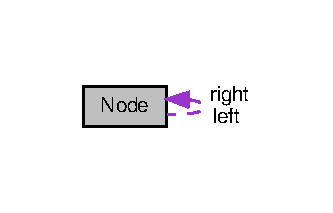
\includegraphics[width=160pt]{structNode__coll__graph}
\end{center}
\end{figure}
\subsection*{Campos de Dados}
\begin{DoxyCompactItemize}
\item 
\mbox{\Hypertarget{structNode_ad88c9a757bfafd5ff265e0837b150056}\label{structNode_ad88c9a757bfafd5ff265e0837b150056}} 
char $\ast$ {\bfseries key}
\item 
\mbox{\Hypertarget{structNode_ad0976834843c7618677d22a10c495b36}\label{structNode_ad0976834843c7618677d22a10c495b36}} 
struct \hyperlink{structNode}{Node} $\ast$ {\bfseries left}
\item 
\mbox{\Hypertarget{structNode_af99e7102380da88d7c079fa264230cf4}\label{structNode_af99e7102380da88d7c079fa264230cf4}} 
struct \hyperlink{structNode}{Node} $\ast$ {\bfseries right}
\item 
\mbox{\Hypertarget{structNode_a61966b207f0584aaa4773e5e1266e905}\label{structNode_a61966b207f0584aaa4773e5e1266e905}} 
int {\bfseries height}
\item 
\mbox{\Hypertarget{structNode_ae08b9529cb7cc71350c9cd80733ded0e}\label{structNode_ae08b9529cb7cc71350c9cd80733ded0e}} 
void $\ast$ {\bfseries equals}
\end{DoxyCompactItemize}


\subsection{Descrição detalhada}


Definido na linha 8 do ficheiro tree.\+c.



A documentação para esta estrutura foi gerada a partir do seguinte ficheiro\+:\begin{DoxyCompactItemize}
\item 
\hyperlink{tree_8c}{tree.\+c}\end{DoxyCompactItemize}

\hypertarget{structprodutosPorCliente}{}\section{Referência à estrutura produtos\+Por\+Cliente}
\label{structprodutosPorCliente}\index{produtos\+Por\+Cliente@{produtos\+Por\+Cliente}}
\subsection*{Campos de Dados}
\begin{DoxyCompactItemize}
\item 
\mbox{\Hypertarget{structprodutosPorCliente_a73a3d29e8fd890012b5efb69b01aa362}\label{structprodutosPorCliente_a73a3d29e8fd890012b5efb69b01aa362}} 
char $\ast$ {\bfseries nome}
\item 
\mbox{\Hypertarget{structprodutosPorCliente_a80af2e5b64b9c1cf14d79b0d75bf1d74}\label{structprodutosPorCliente_a80af2e5b64b9c1cf14d79b0d75bf1d74}} 
int {\bfseries quant} \mbox{[}12\mbox{]}
\item 
\mbox{\Hypertarget{structprodutosPorCliente_a59f56c877170ccc26db5168b28647962}\label{structprodutosPorCliente_a59f56c877170ccc26db5168b28647962}} 
int {\bfseries fat} \mbox{[}12\mbox{]}
\end{DoxyCompactItemize}


\subsection{Descrição detalhada}


Definido na linha 18 do ficheiro filial.\+c.



A documentação para esta estrutura foi gerada a partir do seguinte ficheiro\+:\begin{DoxyCompactItemize}
\item 
\hyperlink{filial_8c}{filial.\+c}\end{DoxyCompactItemize}

\hypertarget{structsgv}{}\section{Referência à estrutura sgv}
\label{structsgv}\index{sgv@{sgv}}
\subsection*{Campos de Dados}
\begin{DoxyCompactItemize}
\item 
\mbox{\Hypertarget{structsgv_a0ff5041803e6298d34e3ed308f2b9aeb}\label{structsgv_a0ff5041803e6298d34e3ed308f2b9aeb}} 
char $\ast$ {\bfseries path} \mbox{[}3\mbox{]}
\item 
\mbox{\Hypertarget{structsgv_abe14db8ce7017577d2b181f9c4655f4f}\label{structsgv_abe14db8ce7017577d2b181f9c4655f4f}} 
Dados $\ast$ {\bfseries clientes}
\item 
\mbox{\Hypertarget{structsgv_a3a09e9ce6464adbaf1aca3b89fcc6a75}\label{structsgv_a3a09e9ce6464adbaf1aca3b89fcc6a75}} 
Dados $\ast$ {\bfseries produtos}
\item 
\mbox{\Hypertarget{structsgv_aa47aedd9d6ed5f4910b478c3c622633f}\label{structsgv_aa47aedd9d6ed5f4910b478c3c622633f}} 
VT $\ast$ {\bfseries vendas}
\item 
\mbox{\Hypertarget{structsgv_a995a8da7e322efdf98992a95034d19e7}\label{structsgv_a995a8da7e322efdf98992a95034d19e7}} 
A\+VL $\ast$ {\bfseries faturas}
\item 
\mbox{\Hypertarget{structsgv_a628652f2be4e76e6b8d3d9d12e9c4543}\label{structsgv_a628652f2be4e76e6b8d3d9d12e9c4543}} 
Filial $\ast$ {\bfseries filial} \mbox{[}3\mbox{]}
\end{DoxyCompactItemize}


\subsection{Descrição detalhada}


Definido na linha 4 do ficheiro interface.\+c.



A documentação para esta estrutura foi gerada a partir do seguinte ficheiro\+:\begin{DoxyCompactItemize}
\item 
interface.\+c\end{DoxyCompactItemize}

\hypertarget{structvenda}{}\section{Referência à estrutura venda}
\label{structvenda}\index{venda@{venda}}
\subsection*{Campos de Dados}
\begin{DoxyCompactItemize}
\item 
\mbox{\Hypertarget{structvenda_add75e22efb9b20604c65573f1d441e73}\label{structvenda_add75e22efb9b20604c65573f1d441e73}} 
char $\ast$ {\bfseries produto}
\item 
\mbox{\Hypertarget{structvenda_af67f645bd17cc9cf76ad77f54aee57f9}\label{structvenda_af67f645bd17cc9cf76ad77f54aee57f9}} 
double {\bfseries preco}
\item 
\mbox{\Hypertarget{structvenda_a2a0d7a3f2121806a8a46cbd35977a428}\label{structvenda_a2a0d7a3f2121806a8a46cbd35977a428}} 
int {\bfseries quantidade}
\item 
\mbox{\Hypertarget{structvenda_a7e0ff1d9ead091d7ab34e52f9ca4a1a3}\label{structvenda_a7e0ff1d9ead091d7ab34e52f9ca4a1a3}} 
char {\bfseries promocao}
\item 
\mbox{\Hypertarget{structvenda_aabfaf980412c727ebe7264a5ac4a0b94}\label{structvenda_aabfaf980412c727ebe7264a5ac4a0b94}} 
char $\ast$ {\bfseries cliente}
\item 
\mbox{\Hypertarget{structvenda_ad4dc58fae65ac2626e005dd316413e5d}\label{structvenda_ad4dc58fae65ac2626e005dd316413e5d}} 
int {\bfseries data}
\item 
\mbox{\Hypertarget{structvenda_ad70ca7868cde668c9c1fa80fe26af6ba}\label{structvenda_ad70ca7868cde668c9c1fa80fe26af6ba}} 
int {\bfseries filial}
\end{DoxyCompactItemize}


\subsection{Descrição detalhada}


Definido na linha 7 do ficheiro vendas.\+c.



A documentação para esta estrutura foi gerada a partir do seguinte ficheiro\+:\begin{DoxyCompactItemize}
\item 
\hyperlink{vendas_8c}{vendas.\+c}\end{DoxyCompactItemize}

\hypertarget{structvt}{}\section{Referência à estrutura vt}
\label{structvt}\index{vt@{vt}}
\subsection*{Campos de Dados}
\begin{DoxyCompactItemize}
\item 
\mbox{\Hypertarget{structvt_a7c75b73cdfe0409780710641680ada56}\label{structvt_a7c75b73cdfe0409780710641680ada56}} 
int {\bfseries size}
\item 
\mbox{\Hypertarget{structvt_a84ca9dd32424d994897b1eee0ca9d672}\label{structvt_a84ca9dd32424d994897b1eee0ca9d672}} 
int {\bfseries ocupados}
\item 
\mbox{\Hypertarget{structvt_aa81d3e2f691fd8892303b35aac1a9e97}\label{structvt_aa81d3e2f691fd8892303b35aac1a9e97}} 
int {\bfseries lidas}
\item 
\mbox{\Hypertarget{structvt_a989d4dcb38eed0d716626f52a972af08}\label{structvt_a989d4dcb38eed0d716626f52a972af08}} 
Venda $\ast$ {\bfseries str}
\end{DoxyCompactItemize}


\subsection{Descrição detalhada}


Definido na linha 18 do ficheiro vendas.\+c.



A documentação para esta estrutura foi gerada a partir do seguinte ficheiro\+:\begin{DoxyCompactItemize}
\item 
\hyperlink{vendas_8c}{vendas.\+c}\end{DoxyCompactItemize}

\chapter{Documentação do ficheiro}
\hypertarget{clientes_8c}{}\section{Referência ao ficheiro clientes.\+c}
\label{clientes_8c}\index{clientes.\+c@{clientes.\+c}}


Ficheiro que contem funções utilizadas para os clientes.  


{\ttfamily \#include \char`\"{}clientes.\+h\char`\"{}}\newline
Diagrama de dependências de inclusão para clientes.\+c\+:
\nopagebreak
\begin{figure}[H]
\begin{center}
\leavevmode
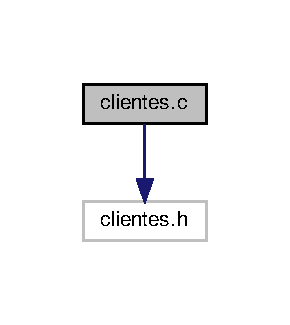
\includegraphics[width=139pt]{clientes_8c__incl}
\end{center}
\end{figure}
\subsection*{Funções}
\begin{DoxyCompactItemize}
\item 
Dados $\ast$ \hyperlink{clientes_8c_ab5e7eab04f090f920f5ea98c6cb1a505}{init\+Dados} ()
\begin{DoxyCompactList}\small\item\em Inicialização dos dados dos clientes. \end{DoxyCompactList}\item 
void \hyperlink{clientes_8c_ab0e31c59339ab5320753ed2e47b91a86}{free\+Dados} (Dados $\ast$l)
\begin{DoxyCompactList}\small\item\em Função que desaloca a memória ocupada pelos Dados. \end{DoxyCompactList}\item 
void \hyperlink{clientes_8c_ab93f3f48a62ea57a21aa91347dc699c7}{realloc\+Dados} (Dados $\ast$lista)
\begin{DoxyCompactList}\small\item\em Função que realoca a memoria ocupada pelos Dados. \end{DoxyCompactList}\item 
int \hyperlink{clientes_8c_a6f76df6572f78ed7afe910732203b41f}{my\+Compare} (const void $\ast$a, const void $\ast$b)
\begin{DoxyCompactList}\small\item\em Função que compara duas constantes. \end{DoxyCompactList}\item 
int \hyperlink{clientes_8c_a5d64af1341f9530f382d2fd3d0fc9dde}{valid\+\_\+\+Clientes} (char $\ast$str)
\begin{DoxyCompactList}\small\item\em Valida os clientes. \end{DoxyCompactList}\item 
void \hyperlink{clientes_8c_a39d3b1a8a7a80fa0eb72d05c9d638110}{read\+\_\+\+Clientes} (Dados $\ast$clientes, char $\ast$file\+Path)
\begin{DoxyCompactList}\small\item\em Função que lê um ficheiro .txt com a informacao relativa aos clientes. \end{DoxyCompactList}\item 
int \hyperlink{clientes_8c_a6750303c5f269b2426b738337b1d7801}{get\+OcupadosC} (Dados $\ast$clientes)
\begin{DoxyCompactList}\small\item\em Função que devolve o espaço ocupado pelos clientes na string. \end{DoxyCompactList}\item 
int \hyperlink{clientes_8c_a1d7c66163d12b2ea478a59f0ba366388}{get\+SizeC} (Dados $\ast$clientes)
\begin{DoxyCompactList}\small\item\em Função que obtem o tamanho da string. \end{DoxyCompactList}\item 
int \hyperlink{clientes_8c_ab90d042b32e5c60ef85c6b1341b8a1b5}{get\+LidasC} (Dados $\ast$clientes)
\begin{DoxyCompactList}\small\item\em Função que devolve os clientes lidos. \end{DoxyCompactList}\item 
char $\ast$ \hyperlink{clientes_8c_a606370124e1d3d3b932d857296710829}{get\+ClienteC} (int i, Dados $\ast$clientes)
\begin{DoxyCompactList}\small\item\em Função que devolve um array com os clientes. \end{DoxyCompactList}\item 
\mbox{\Hypertarget{clientes_8c_a00913187525d42aa3bb739d35000a2f5}\label{clientes_8c_a00913187525d42aa3bb739d35000a2f5}} 
char $\ast$$\ast$ {\bfseries get\+S\+T\+Rdos\+Clientes} (Dados $\ast$clientes)
\end{DoxyCompactItemize}


\subsection{Descrição detalhada}
Ficheiro que contem funções utilizadas para os clientes. 

Ficheiro utilizado para imprimir os outputs das funçóes.

\subsection{Documentação das funções}
\mbox{\Hypertarget{clientes_8c_ab0e31c59339ab5320753ed2e47b91a86}\label{clientes_8c_ab0e31c59339ab5320753ed2e47b91a86}} 
\index{clientes.\+c@{clientes.\+c}!free\+Dados@{free\+Dados}}
\index{free\+Dados@{free\+Dados}!clientes.\+c@{clientes.\+c}}
\subsubsection{\texorpdfstring{free\+Dados()}{freeDados()}}
{\footnotesize\ttfamily void free\+Dados (\begin{DoxyParamCaption}\item[{Dados $\ast$}]{l }\end{DoxyParamCaption})}



Função que desaloca a memória ocupada pelos Dados. 


\begin{DoxyParams}{Parâmetros}
{\em \mbox{[}d\mbox{]}} & Dados \\
\hline
\end{DoxyParams}


Definido na linha 37 do ficheiro clientes.\+c.


\begin{DoxyCode}
37                         \{
38     \textcolor{keywordtype}{int} i;
39     \textcolor{keywordflow}{for}(i = 0;i<l->ocupados;i++)
40         free(l->str[i]);
41     free(l->str);
42     free(l);
43 \}
\end{DoxyCode}
\mbox{\Hypertarget{clientes_8c_a606370124e1d3d3b932d857296710829}\label{clientes_8c_a606370124e1d3d3b932d857296710829}} 
\index{clientes.\+c@{clientes.\+c}!get\+ClienteC@{get\+ClienteC}}
\index{get\+ClienteC@{get\+ClienteC}!clientes.\+c@{clientes.\+c}}
\subsubsection{\texorpdfstring{get\+Cliente\+C()}{getClienteC()}}
{\footnotesize\ttfamily char$\ast$ get\+ClienteC (\begin{DoxyParamCaption}\item[{int}]{i,  }\item[{Dados $\ast$}]{clientes }\end{DoxyParamCaption})}



Função que devolve um array com os clientes. 


\begin{DoxyParams}{Parâmetros}
{\em \mbox{[}i\mbox{]}} & Indíce do array str \\
\hline
{\em \mbox{[}clientes\mbox{]}} & Dados dos clientes \\
\hline
\end{DoxyParams}
\begin{DoxyReturn}{Retorna}
Array com os clientes 
\end{DoxyReturn}


Definido na linha 168 do ficheiro clientes.\+c.


\begin{DoxyCode}
168                                          \{
169   \textcolor{keywordflow}{return} strdup(clientes->str[i]);
170 \}
\end{DoxyCode}
\mbox{\Hypertarget{clientes_8c_ab90d042b32e5c60ef85c6b1341b8a1b5}\label{clientes_8c_ab90d042b32e5c60ef85c6b1341b8a1b5}} 
\index{clientes.\+c@{clientes.\+c}!get\+LidasC@{get\+LidasC}}
\index{get\+LidasC@{get\+LidasC}!clientes.\+c@{clientes.\+c}}
\subsubsection{\texorpdfstring{get\+Lidas\+C()}{getLidasC()}}
{\footnotesize\ttfamily int get\+LidasC (\begin{DoxyParamCaption}\item[{Dados $\ast$}]{clientes }\end{DoxyParamCaption})}



Função que devolve os clientes lidos. 


\begin{DoxyParams}{Parâmetros}
{\em \mbox{[}produtos\mbox{]}} & Dados dos clientes \\
\hline
\end{DoxyParams}
\begin{DoxyReturn}{Retorna}
Clientes lidos 
\end{DoxyReturn}


Definido na linha 158 do ficheiro clientes.\+c.


\begin{DoxyCode}
158                                \{
159   \textcolor{keywordflow}{return} clientes->lidas;
160 \}
\end{DoxyCode}
\mbox{\Hypertarget{clientes_8c_a6750303c5f269b2426b738337b1d7801}\label{clientes_8c_a6750303c5f269b2426b738337b1d7801}} 
\index{clientes.\+c@{clientes.\+c}!get\+OcupadosC@{get\+OcupadosC}}
\index{get\+OcupadosC@{get\+OcupadosC}!clientes.\+c@{clientes.\+c}}
\subsubsection{\texorpdfstring{get\+Ocupados\+C()}{getOcupadosC()}}
{\footnotesize\ttfamily int get\+OcupadosC (\begin{DoxyParamCaption}\item[{Dados $\ast$}]{clientes }\end{DoxyParamCaption})}



Função que devolve o espaço ocupado pelos clientes na string. 


\begin{DoxyParams}{Parâmetros}
{\em \mbox{[}produtos\mbox{]}} & Dados dos clientes \\
\hline
\end{DoxyParams}
\begin{DoxyReturn}{Retorna}
Espaço ocupado pelos produtos na string 
\end{DoxyReturn}


Definido na linha 140 do ficheiro clientes.\+c.


\begin{DoxyCode}
140                                   \{
141   \textcolor{keywordflow}{return} clientes->ocupados;
142 \}
\end{DoxyCode}
\mbox{\Hypertarget{clientes_8c_a1d7c66163d12b2ea478a59f0ba366388}\label{clientes_8c_a1d7c66163d12b2ea478a59f0ba366388}} 
\index{clientes.\+c@{clientes.\+c}!get\+SizeC@{get\+SizeC}}
\index{get\+SizeC@{get\+SizeC}!clientes.\+c@{clientes.\+c}}
\subsubsection{\texorpdfstring{get\+Size\+C()}{getSizeC()}}
{\footnotesize\ttfamily int get\+SizeC (\begin{DoxyParamCaption}\item[{Dados $\ast$}]{clientes }\end{DoxyParamCaption})}



Função que obtem o tamanho da string. 


\begin{DoxyParams}{Parâmetros}
{\em \mbox{[}clientes\mbox{]}} & Dados dos clientes \\
\hline
\end{DoxyParams}
\begin{DoxyReturn}{Retorna}
Tamanho da string 
\end{DoxyReturn}


Definido na linha 149 do ficheiro clientes.\+c.


\begin{DoxyCode}
149                               \{
150   \textcolor{keywordflow}{return} clientes->ocupados;
151 \}
\end{DoxyCode}
\mbox{\Hypertarget{clientes_8c_ab5e7eab04f090f920f5ea98c6cb1a505}\label{clientes_8c_ab5e7eab04f090f920f5ea98c6cb1a505}} 
\index{clientes.\+c@{clientes.\+c}!init\+Dados@{init\+Dados}}
\index{init\+Dados@{init\+Dados}!clientes.\+c@{clientes.\+c}}
\subsubsection{\texorpdfstring{init\+Dados()}{initDados()}}
{\footnotesize\ttfamily Dados$\ast$ init\+Dados (\begin{DoxyParamCaption}{ }\end{DoxyParamCaption})}



Inicialização dos dados dos clientes. 

\begin{DoxyReturn}{Retorna}
Novo dado 
\end{DoxyReturn}


Definido na linha 12 do ficheiro clientes.\+c.


\begin{DoxyCode}
12                    \{
13   Dados* d = malloc(\textcolor{keyword}{sizeof}(Dados));
14   d->size = 1;
15   d->ocupados = 0;
16   d->lidas = 0;
17   d->str = malloc(\textcolor{keyword}{sizeof}(\textcolor{keywordtype}{char}*));
18   \textcolor{keywordflow}{return} d;
19 \}
\end{DoxyCode}
\mbox{\Hypertarget{clientes_8c_a6f76df6572f78ed7afe910732203b41f}\label{clientes_8c_a6f76df6572f78ed7afe910732203b41f}} 
\index{clientes.\+c@{clientes.\+c}!my\+Compare@{my\+Compare}}
\index{my\+Compare@{my\+Compare}!clientes.\+c@{clientes.\+c}}
\subsubsection{\texorpdfstring{my\+Compare()}{myCompare()}}
{\footnotesize\ttfamily int my\+Compare (\begin{DoxyParamCaption}\item[{const void $\ast$}]{a,  }\item[{const void $\ast$}]{b }\end{DoxyParamCaption})}



Função que compara duas constantes. 


\begin{DoxyParams}{Parâmetros}
{\em \mbox{[}a\mbox{]}} & Uma constante \\
\hline
{\em \mbox{[}b\mbox{]}} & Uma constante \\
\hline
\end{DoxyParams}
\begin{DoxyReturn}{Retorna}
Resultado desta comparação 
\end{DoxyReturn}


Definido na linha 81 do ficheiro clientes.\+c.


\begin{DoxyCode}
81                                                 \{
82     \textcolor{keyword}{const} \textcolor{keywordtype}{char} *pa = *(\textcolor{keyword}{const} \textcolor{keywordtype}{char}**)a;
83     \textcolor{keyword}{const} \textcolor{keywordtype}{char} *pb = *(\textcolor{keyword}{const} \textcolor{keywordtype}{char}**)b;
84 
85     \textcolor{keywordflow}{return} strcmp(pa,pb);
86 \}
\end{DoxyCode}
\mbox{\Hypertarget{clientes_8c_a39d3b1a8a7a80fa0eb72d05c9d638110}\label{clientes_8c_a39d3b1a8a7a80fa0eb72d05c9d638110}} 
\index{clientes.\+c@{clientes.\+c}!read\+\_\+\+Clientes@{read\+\_\+\+Clientes}}
\index{read\+\_\+\+Clientes@{read\+\_\+\+Clientes}!clientes.\+c@{clientes.\+c}}
\subsubsection{\texorpdfstring{read\+\_\+\+Clientes()}{read\_Clientes()}}
{\footnotesize\ttfamily void read\+\_\+\+Clientes (\begin{DoxyParamCaption}\item[{Dados $\ast$}]{clientes,  }\item[{char $\ast$}]{file\+Path }\end{DoxyParamCaption})}



Função que lê um ficheiro .txt com a informacao relativa aos clientes. 


\begin{DoxyParams}{Parâmetros}
{\em \mbox{[}clientes\mbox{]}} & Dados dos clientes \\
\hline
{\em \mbox{[}file\+Path\mbox{]}} & Caminho do ficheiro \\
\hline
\end{DoxyParams}


Definido na linha 112 do ficheiro clientes.\+c.


\begin{DoxyCode}
112                                                     \{
113   FILE* f = fopen(filePath, \textcolor{stringliteral}{"r"});
114   \textcolor{keywordflow}{if} (f == NULL)\{
115     printf(\textcolor{stringliteral}{"Ficheiro clientes inexistente\(\backslash\)n"});
116   \}
117   \textcolor{keywordtype}{char} str[1024];
118 
119   \textcolor{keywordflow}{while}(fgets(str,1024,f))\{
120     clientes->lidas++;
121     \textcolor{keywordflow}{if}(\hyperlink{clientes_8c_a5d64af1341f9530f382d2fd3d0fc9dde}{valid\_Clientes}(strtok(str,\textcolor{stringliteral}{"\(\backslash\)r\(\backslash\)n"})) == 1)\{
122       \textcolor{keywordflow}{if}(clientes->size == clientes->ocupados)\{
123         \hyperlink{clientes_8c_ab93f3f48a62ea57a21aa91347dc699c7}{reallocDados}(clientes);
124       \}
125       clientes->str[clientes->ocupados] = strdup(str);
126       clientes->ocupados++;
127 
128     \}
129   \}
130   qsort(clientes->str,clientes->ocupados,\textcolor{keyword}{sizeof}(\textcolor{keywordtype}{char}*),\hyperlink{clientes_8c_a6f76df6572f78ed7afe910732203b41f}{myCompare});
131   fclose(f);
132 \}
\end{DoxyCode}
\mbox{\Hypertarget{clientes_8c_ab93f3f48a62ea57a21aa91347dc699c7}\label{clientes_8c_ab93f3f48a62ea57a21aa91347dc699c7}} 
\index{clientes.\+c@{clientes.\+c}!realloc\+Dados@{realloc\+Dados}}
\index{realloc\+Dados@{realloc\+Dados}!clientes.\+c@{clientes.\+c}}
\subsubsection{\texorpdfstring{realloc\+Dados()}{reallocDados()}}
{\footnotesize\ttfamily void realloc\+Dados (\begin{DoxyParamCaption}\item[{Dados $\ast$}]{lista }\end{DoxyParamCaption})}



Função que realoca a memoria ocupada pelos Dados. 


\begin{DoxyParams}{Parâmetros}
{\em \mbox{[}d\mbox{]}} & Dados \\
\hline
\end{DoxyParams}


Definido na linha 63 do ficheiro clientes.\+c.


\begin{DoxyCode}
63                                \{
64     \textcolor{keywordtype}{int} i;
65     \textcolor{keywordtype}{char} **tmp = malloc(2*lista->size*\textcolor{keyword}{sizeof}(\textcolor{keywordtype}{char}*));
66     \textcolor{keywordflow}{for}(i = 0;i<lista->size;i++)\{
67         tmp[i] = lista->str[i];
68     \}
69     free(lista->str);
70     lista->str = tmp;
71     lista->size *=2;
72 \}
\end{DoxyCode}
\mbox{\Hypertarget{clientes_8c_a5d64af1341f9530f382d2fd3d0fc9dde}\label{clientes_8c_a5d64af1341f9530f382d2fd3d0fc9dde}} 
\index{clientes.\+c@{clientes.\+c}!valid\+\_\+\+Clientes@{valid\+\_\+\+Clientes}}
\index{valid\+\_\+\+Clientes@{valid\+\_\+\+Clientes}!clientes.\+c@{clientes.\+c}}
\subsubsection{\texorpdfstring{valid\+\_\+\+Clientes()}{valid\_Clientes()}}
{\footnotesize\ttfamily int valid\+\_\+\+Clientes (\begin{DoxyParamCaption}\item[{char $\ast$}]{str }\end{DoxyParamCaption})}



Valida os clientes. 


\begin{DoxyParams}{Parâmetros}
{\em \mbox{[}str\mbox{]}} & Código de um cliente \\
\hline
\end{DoxyParams}
\begin{DoxyReturn}{Retorna}
Um r que nos diz se um cliente é valido (r=1) ou invalido (r=0) 
\end{DoxyReturn}


Definido na linha 94 do ficheiro clientes.\+c.


\begin{DoxyCode}
94                               \{
95   \textcolor{keywordtype}{int} i,r = 1;
96   \textcolor{keywordtype}{int} l = strlen(str);
97   \textcolor{keywordflow}{if} (l == 5 && (isupper(str[0])) > 0) \{
98     \textcolor{keywordflow}{for} (i = 1; i < l-1 && r == 1; i++)\{
99       \textcolor{keywordflow}{if} (!(isdigit(str[i]))) r = 0;
100     \}
101   \}
102   \textcolor{keywordflow}{else} r = 0;
103   \textcolor{keywordflow}{return} r;
104 \}
\end{DoxyCode}

\hypertarget{faturacao_8c}{}\section{Referência ao ficheiro faturacao.\+c}
\label{faturacao_8c}\index{faturacao.\+c@{faturacao.\+c}}


Modulo que inicializa e controi a estrutura faturacao.  


{\ttfamily \#include \char`\"{}faturacao.\+h\char`\"{}}\newline
Diagrama de dependências de inclusão para faturacao.\+c\+:
\nopagebreak
\begin{figure}[H]
\begin{center}
\leavevmode
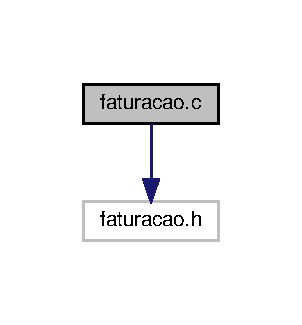
\includegraphics[width=145pt]{faturacao_8c__incl}
\end{center}
\end{figure}
\subsection*{Estruturas de Dados}
\begin{DoxyCompactItemize}
\item 
struct \hyperlink{structfatura}{fatura}
\end{DoxyCompactItemize}
\subsection*{Funções}
\begin{DoxyCompactItemize}
\item 
\mbox{\Hypertarget{faturacao_8c_af10828b406e4e74b89b821e189452bc3}\label{faturacao_8c_af10828b406e4e74b89b821e189452bc3}} 
void {\bfseries free\+Nodo\+A\+V\+L\+Fatura} (Fatura $\ast$f)
\item 
void \hyperlink{faturacao_8c_a4ac6ba9606cd84ea8d0b137b059f8756}{insere\+Fatura} (Fatura $\ast$f, Venda $\ast$v)
\begin{DoxyCompactList}\small\item\em Insere uma venda numa fatura. \end{DoxyCompactList}\item 
Fatura $\ast$ \hyperlink{faturacao_8c_abb686b9175c00f86f3bce095854aa18a}{init\+Fatura} ()
\begin{DoxyCompactList}\small\item\em Inicialização das faturas. \end{DoxyCompactList}\item 
Fatura $\ast$ \hyperlink{faturacao_8c_a7976d6439bd69bcce0b52d3fe05a8a2d}{clone\+Faturas} (Fatura $\ast$f)
\begin{DoxyCompactList}\small\item\em Cria um clone de uma fatura. \end{DoxyCompactList}\item 
char $\ast$ \hyperlink{faturacao_8c_ad55844e4e49d564972bb0a537b4ad23b}{get\+Produto\+Fatura} (Fatura $\ast$f)
\begin{DoxyCompactList}\small\item\em Retorna o produto de uma fatura. \end{DoxyCompactList}\item 
int \hyperlink{faturacao_8c_afb82689eef0b05cad519049a05d50eeb}{get\+Numero\+Total\+Vendas} (Fatura $\ast$f, int \hyperlink{structfilial}{filial}, int mes, int prom)
\begin{DoxyCompactList}\small\item\em Obtem o numero total de vendas dado o mês, a filial e o tipo de promoção. \end{DoxyCompactList}\item 
int \hyperlink{faturacao_8c_a5e2ddbc2467f7b0df879e5f0e84878ef}{get\+Quantidade\+P\+Filial} (Fatura $\ast$f, int \hyperlink{structfilial}{filial})
\begin{DoxyCompactList}\small\item\em Obtem a quantidade total dada a filial. \end{DoxyCompactList}\item 
double \hyperlink{faturacao_8c_a23224f16d2f9428fbff8de49592c0f9e}{get\+Faturacao} (Fatura $\ast$f, int \hyperlink{structfilial}{filial}, int mes, int prom)
\begin{DoxyCompactList}\small\item\em Obtem a faturacao total dado o mês, a filial e o tipo de promoção. \end{DoxyCompactList}\end{DoxyCompactItemize}


\subsection{Descrição detalhada}
Modulo que inicializa e controi a estrutura faturacao. 



\subsection{Documentação das funções}
\mbox{\Hypertarget{faturacao_8c_a7976d6439bd69bcce0b52d3fe05a8a2d}\label{faturacao_8c_a7976d6439bd69bcce0b52d3fe05a8a2d}} 
\index{faturacao.\+c@{faturacao.\+c}!clone\+Faturas@{clone\+Faturas}}
\index{clone\+Faturas@{clone\+Faturas}!faturacao.\+c@{faturacao.\+c}}
\subsubsection{\texorpdfstring{clone\+Faturas()}{cloneFaturas()}}
{\footnotesize\ttfamily Fatura$\ast$ clone\+Faturas (\begin{DoxyParamCaption}\item[{Fatura $\ast$}]{f }\end{DoxyParamCaption})}



Cria um clone de uma fatura. 


\begin{DoxyParams}{Parâmetros}
{\em \mbox{[}f\mbox{]}} & Fatura que vai ser clonizada \\
\hline
\end{DoxyParams}
\begin{DoxyReturn}{Retorna}
Fatura clone 
\end{DoxyReturn}


Definido na linha 63 do ficheiro faturacao.\+c.


\begin{DoxyCode}
63                                \{
64   Fatura* a = malloc(\textcolor{keyword}{sizeof}(Fatura));
65   \textcolor{keywordtype}{int} i, j, k;
66   a->produto = strdup(f->produto);
67   \textcolor{keywordflow}{for}(i = 0; i < 3; i++)\{
68     a->quantPorFilial[i] = f->quantPorFilial[i];
69     \textcolor{keywordflow}{for}(j = 0; j < 12; j++)\{
70       \textcolor{keywordflow}{for}(k = 0; k < 2; k++)\{
71         a->numeroTotalVendas[i][j][k] = f->numeroTotalVendas[i][j][k];
72         a->faturaTotal[i][j][k] = f->faturaTotal[i][j][k];
73       \}
74     \}
75   \}
76   \textcolor{keywordflow}{return} a;
77 \}
\end{DoxyCode}
\mbox{\Hypertarget{faturacao_8c_a23224f16d2f9428fbff8de49592c0f9e}\label{faturacao_8c_a23224f16d2f9428fbff8de49592c0f9e}} 
\index{faturacao.\+c@{faturacao.\+c}!get\+Faturacao@{get\+Faturacao}}
\index{get\+Faturacao@{get\+Faturacao}!faturacao.\+c@{faturacao.\+c}}
\subsubsection{\texorpdfstring{get\+Faturacao()}{getFaturacao()}}
{\footnotesize\ttfamily double get\+Faturacao (\begin{DoxyParamCaption}\item[{Fatura $\ast$}]{f,  }\item[{int}]{filial,  }\item[{int}]{mes,  }\item[{int}]{prom }\end{DoxyParamCaption})}



Obtem a faturacao total dado o mês, a filial e o tipo de promoção. 


\begin{DoxyParams}{Parâmetros}
{\em \mbox{[}f\mbox{]}} & Estrutura fatura \\
\hline
{\em \mbox{[}filial\mbox{]}} & Inteiro que determina a filial (filial = 0 -\/$>$ todas as filials) \\
\hline
{\em \mbox{[}mes\mbox{]}} & Inteiro que determina o mes \\
\hline
{\em \mbox{[}prom\mbox{]}} & Inteiro que determina a tipo de promocao (prom = 0 -\/$>$ N e prom = 1 -\/$>$ P) \\
\hline
\end{DoxyParams}
\begin{DoxyReturn}{Retorna}
Retorna a faturacao total 
\end{DoxyReturn}


Definido na linha 123 do ficheiro faturacao.\+c.


\begin{DoxyCode}
123                                                               \{
124   \textcolor{keywordflow}{if}(\hyperlink{structfilial}{filial} == 0)
125     \textcolor{keywordflow}{return} f->faturaTotal[0][mes-1][prom] + f->faturaTotal[1][mes-1][prom] + f->faturaTotal[2][mes-1][prom]
      ;
126 
127   \textcolor{keywordflow}{return} f->faturaTotal[\hyperlink{structfilial}{filial}-1][mes-1][prom];
128 \}
\end{DoxyCode}
\mbox{\Hypertarget{faturacao_8c_afb82689eef0b05cad519049a05d50eeb}\label{faturacao_8c_afb82689eef0b05cad519049a05d50eeb}} 
\index{faturacao.\+c@{faturacao.\+c}!get\+Numero\+Total\+Vendas@{get\+Numero\+Total\+Vendas}}
\index{get\+Numero\+Total\+Vendas@{get\+Numero\+Total\+Vendas}!faturacao.\+c@{faturacao.\+c}}
\subsubsection{\texorpdfstring{get\+Numero\+Total\+Vendas()}{getNumeroTotalVendas()}}
{\footnotesize\ttfamily int get\+Numero\+Total\+Vendas (\begin{DoxyParamCaption}\item[{Fatura $\ast$}]{f,  }\item[{int}]{filial,  }\item[{int}]{mes,  }\item[{int}]{prom }\end{DoxyParamCaption})}



Obtem o numero total de vendas dado o mês, a filial e o tipo de promoção. 


\begin{DoxyParams}{Parâmetros}
{\em \mbox{[}f\mbox{]}} & Estrutura fatura \\
\hline
{\em \mbox{[}filial\mbox{]}} & Inteiro que determina a filial (filial = 0 -\/$>$ todas as filials) \\
\hline
{\em \mbox{[}mes\mbox{]}} & Inteiro que determina o mes \\
\hline
{\em \mbox{[}prom\mbox{]}} & Inteiro que determina a tipo de promocao (prom = 0 -\/$>$ N e prom = 1 -\/$>$ P) \\
\hline
\end{DoxyParams}
\begin{DoxyReturn}{Retorna}
Retorna o numero total de vendas 
\end{DoxyReturn}


Definido na linha 96 do ficheiro faturacao.\+c.


\begin{DoxyCode}
96                                                                    \{
97   \textcolor{keywordflow}{if}(\hyperlink{structfilial}{filial} == 0)
98     \textcolor{keywordflow}{return} f->numeroTotalVendas[0][mes-1][prom]+f->numeroTotalVendas[1][mes-1][prom]+ f->numeroTotalVendas[
      2][mes-1][prom];
99   \textcolor{keywordflow}{return} f->numeroTotalVendas[\hyperlink{structfilial}{filial}-1][mes-1][prom];
100 \}
\end{DoxyCode}
\mbox{\Hypertarget{faturacao_8c_ad55844e4e49d564972bb0a537b4ad23b}\label{faturacao_8c_ad55844e4e49d564972bb0a537b4ad23b}} 
\index{faturacao.\+c@{faturacao.\+c}!get\+Produto\+Fatura@{get\+Produto\+Fatura}}
\index{get\+Produto\+Fatura@{get\+Produto\+Fatura}!faturacao.\+c@{faturacao.\+c}}
\subsubsection{\texorpdfstring{get\+Produto\+Fatura()}{getProdutoFatura()}}
{\footnotesize\ttfamily char$\ast$ get\+Produto\+Fatura (\begin{DoxyParamCaption}\item[{Fatura $\ast$}]{f }\end{DoxyParamCaption})}



Retorna o produto de uma fatura. 


\begin{DoxyParams}{Parâmetros}
{\em \mbox{[}f\mbox{]}} & Estrutura fatura \\
\hline
\end{DoxyParams}
\begin{DoxyReturn}{Retorna}
Produto de uma fatura 
\end{DoxyReturn}


Definido na linha 84 do ficheiro faturacao.\+c.


\begin{DoxyCode}
84                                  \{
85   \textcolor{keywordflow}{return} f->produto;
86 \}
\end{DoxyCode}
\mbox{\Hypertarget{faturacao_8c_a5e2ddbc2467f7b0df879e5f0e84878ef}\label{faturacao_8c_a5e2ddbc2467f7b0df879e5f0e84878ef}} 
\index{faturacao.\+c@{faturacao.\+c}!get\+Quantidade\+P\+Filial@{get\+Quantidade\+P\+Filial}}
\index{get\+Quantidade\+P\+Filial@{get\+Quantidade\+P\+Filial}!faturacao.\+c@{faturacao.\+c}}
\subsubsection{\texorpdfstring{get\+Quantidade\+P\+Filial()}{getQuantidadePFilial()}}
{\footnotesize\ttfamily int get\+Quantidade\+P\+Filial (\begin{DoxyParamCaption}\item[{Fatura $\ast$}]{f,  }\item[{int}]{filial }\end{DoxyParamCaption})}



Obtem a quantidade total dada a filial. 


\begin{DoxyParams}{Parâmetros}
{\em \mbox{[}f\mbox{]}} & Estrutura fatura \\
\hline
{\em \mbox{[}filial\mbox{]}} & Inteiro que determina a filial (filial = 0 -\/$>$ todas as filials) \\
\hline
\end{DoxyParams}
\begin{DoxyReturn}{Retorna}
Retorna a faturacao total 
\end{DoxyReturn}


Definido na linha 109 do ficheiro faturacao.\+c.


\begin{DoxyCode}
109                                                \{
110   \textcolor{keywordflow}{if} (\hyperlink{structfilial}{filial} == 0)
111     \textcolor{keywordflow}{return} f->quantPorFilial[0]+f->quantPorFilial[1]+f->quantPorFilial[2];
112   \textcolor{keywordflow}{return} f->quantPorFilial[\hyperlink{structfilial}{filial}-1];
113 \}
\end{DoxyCode}
\mbox{\Hypertarget{faturacao_8c_abb686b9175c00f86f3bce095854aa18a}\label{faturacao_8c_abb686b9175c00f86f3bce095854aa18a}} 
\index{faturacao.\+c@{faturacao.\+c}!init\+Fatura@{init\+Fatura}}
\index{init\+Fatura@{init\+Fatura}!faturacao.\+c@{faturacao.\+c}}
\subsubsection{\texorpdfstring{init\+Fatura()}{initFatura()}}
{\footnotesize\ttfamily Fatura$\ast$ init\+Fatura (\begin{DoxyParamCaption}{ }\end{DoxyParamCaption})}



Inicialização das faturas. 

\begin{DoxyReturn}{Retorna}
Nova fatura 
\end{DoxyReturn}


Definido na linha 43 do ficheiro faturacao.\+c.


\begin{DoxyCode}
43                      \{
44   \textcolor{keywordtype}{int} i,j,k;
45   Fatura* f = malloc(\textcolor{keyword}{sizeof}(Fatura));
46   \textcolor{keywordflow}{for}(i = 0; i < 3; i++)\{
47     f->quantPorFilial[i] = 0;
48     \textcolor{keywordflow}{for}(j = 0; j < 12; j++)\{
49       \textcolor{keywordflow}{for}(k = 0; k < 2; k++)\{
50         f->numeroTotalVendas[i][j][k] = 0;
51         f->faturaTotal[i][j][k] = 0;
52       \}
53     \}
54   \}
55   \textcolor{keywordflow}{return} f;
56 \}
\end{DoxyCode}
\mbox{\Hypertarget{faturacao_8c_a4ac6ba9606cd84ea8d0b137b059f8756}\label{faturacao_8c_a4ac6ba9606cd84ea8d0b137b059f8756}} 
\index{faturacao.\+c@{faturacao.\+c}!insere\+Fatura@{insere\+Fatura}}
\index{insere\+Fatura@{insere\+Fatura}!faturacao.\+c@{faturacao.\+c}}
\subsubsection{\texorpdfstring{insere\+Fatura()}{insereFatura()}}
{\footnotesize\ttfamily void insere\+Fatura (\begin{DoxyParamCaption}\item[{Fatura $\ast$}]{f,  }\item[{Venda $\ast$}]{v }\end{DoxyParamCaption})}



Insere uma venda numa fatura. 


\begin{DoxyParams}{Parâmetros}
{\em \mbox{[}f\mbox{]}} & Estrutura fatura \\
\hline
{\em \mbox{[}v\mbox{]}} & Estrutura venda que vai ser inserida. \\
\hline
\end{DoxyParams}


Definido na linha 28 do ficheiro faturacao.\+c.


\begin{DoxyCode}
28                                        \{
29   \textcolor{keywordtype}{int} data,\hyperlink{structfilial}{filial},prom;
30   data = \hyperlink{vendas_8c_a1178cf1dea33bcb6c9612d46f7534f33}{getData}(v);
31   filial = \hyperlink{vendas_8c_a7381c97aa7302d679514ddbeabb1753f}{getFilial}(v);
32   prom = \hyperlink{vendas_8c_ac48ab849f5af46f09394a208f41029e6}{getPromocao}(v);
33   f->produto = \hyperlink{vendas_8c_a44aa4bbfb64f14bb33fefaeb575c00e1}{getProduto}(v);
34   f->numeroTotalVendas[filial-1][data-1][prom]++;
35   f->quantPorFilial[filial-1] += \hyperlink{vendas_8c_ae3196cffdcf5289440c1ee56ed5ee0d7}{getQuantidade}(v);
36   f->faturaTotal[filial-1][data-1][prom] += \hyperlink{vendas_8c_a9cde304721e7cf45c51ec95bcf625de4}{getPreco}(v)*\hyperlink{vendas_8c_ae3196cffdcf5289440c1ee56ed5ee0d7}{getQuantidade}(v);
37 \}
\end{DoxyCode}

\hypertarget{faturacoes_8c}{}\section{Referência ao ficheiro faturacoes.\+c}
\label{faturacoes_8c}\index{faturacoes.\+c@{faturacoes.\+c}}


Modulo que inicializa e insere as estruturas faturas numa estrutura A\+VL.  


{\ttfamily \#include \char`\"{}faturacoes.\+h\char`\"{}}\newline
Diagrama de dependências de inclusão para faturacoes.\+c\+:
\nopagebreak
\begin{figure}[H]
\begin{center}
\leavevmode
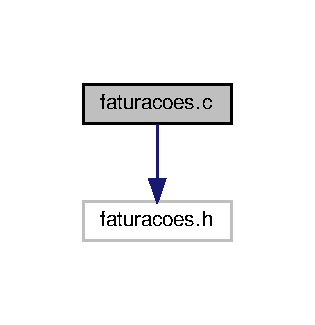
\includegraphics[width=151pt]{faturacoes_8c__incl}
\end{center}
\end{figure}
\subsection*{Funções}
\begin{DoxyCompactItemize}
\item 
void \hyperlink{faturacoes_8c_aa5fa05d951aa26b59256eb8fd0cd23b4}{free\+A\+V\+L\+Fatura} (A\+VL $\ast$f)
\begin{DoxyCompactList}\small\item\em Desaloca a memória ocupada por faturas em A\+VL. \end{DoxyCompactList}\item 
A\+VL $\ast$ \hyperlink{faturacoes_8c_aa807d9f5269922f16e4c4c4747b94ad6}{insere\+Fatura\+A\+VL} (VT $\ast$v, A\+VL $\ast$t)
\begin{DoxyCompactList}\small\item\em Insere a estrutura fatura numa A\+VL. \end{DoxyCompactList}\item 
int \hyperlink{faturacoes_8c_ad0ab422afb76b46b337198cd6ac3d1dc}{get\+Numero\+T\+Vend\+A\+VL} (A\+VL $\ast$a, char $\ast$prod, int \hyperlink{structfilial}{filial}, int mes, int prom)
\begin{DoxyCompactList}\small\item\em Obtem o numero total de vendas dado o mês, a filial e o tipo de promoção recorrendo a A\+VL. \end{DoxyCompactList}\item 
int \hyperlink{faturacoes_8c_ace1cdc0f36557bd0b611ecfc71c987bb}{get\+Quantidade\+P\+Filial\+A\+VL} (A\+VL $\ast$a, char $\ast$prod, int \hyperlink{structfilial}{filial})
\begin{DoxyCompactList}\small\item\em Obtem a quantidade total de produtos vendidos dado o mês, a filial e o tipo de promoção recorrendo a A\+VL. \end{DoxyCompactList}\item 
int \hyperlink{faturacoes_8c_a43188dee2f6d08c9d153fb918bf28a33}{get\+Faturacao\+A\+VL} (A\+VL $\ast$a, char $\ast$prod, int \hyperlink{structfilial}{filial}, int mes, int prom)
\begin{DoxyCompactList}\small\item\em Obtem a faturacao total de vendas dado o mês, a filial e o tipo de promoção recorrendo a A\+VL. \end{DoxyCompactList}\item 
double \hyperlink{faturacoes_8c_af7fa5bf2aa878f4f9f9a7576ce7be824}{faturacao\+T\+A\+VL} (A\+VL $\ast$\hyperlink{structfatura}{fatura}, int min\+Month, int max\+Month)
\begin{DoxyCompactList}\small\item\em Indica-\/nos a faturação dado um intervalo fechado de meses. \end{DoxyCompactList}\item 
int \hyperlink{faturacoes_8c_a818fac565930eaab175228a1cf519e3e}{quantidade\+T\+A\+VL} (A\+VL $\ast$\hyperlink{structfatura}{fatura}, int min\+Month, int max\+Month)
\begin{DoxyCompactList}\small\item\em Indica-\/nos a quantidade dado um intervalo fechado de meses. \end{DoxyCompactList}\end{DoxyCompactItemize}


\subsection{Descrição detalhada}
Modulo que inicializa e insere as estruturas faturas numa estrutura A\+VL. 



\subsection{Documentação das funções}
\mbox{\Hypertarget{faturacoes_8c_af7fa5bf2aa878f4f9f9a7576ce7be824}\label{faturacoes_8c_af7fa5bf2aa878f4f9f9a7576ce7be824}} 
\index{faturacoes.\+c@{faturacoes.\+c}!faturacao\+T\+A\+VL@{faturacao\+T\+A\+VL}}
\index{faturacao\+T\+A\+VL@{faturacao\+T\+A\+VL}!faturacoes.\+c@{faturacoes.\+c}}
\subsubsection{\texorpdfstring{faturacao\+T\+A\+V\+L()}{faturacaoTAVL()}}
{\footnotesize\ttfamily double faturacao\+T\+A\+VL (\begin{DoxyParamCaption}\item[{A\+VL $\ast$}]{fatura,  }\item[{int}]{min\+Month,  }\item[{int}]{max\+Month }\end{DoxyParamCaption})}



Indica-\/nos a faturação dado um intervalo fechado de meses. 


\begin{DoxyParams}{Parâmetros}
{\em \mbox{[}fatura\mbox{]}} & Estrutura A\+VL \\
\hline
{\em \mbox{[}min\+Month\mbox{]}} & Limite inferior \\
\hline
{\em \mbox{[}max\+Month\mbox{]}} & Limite superior \\
\hline
\end{DoxyParams}
\begin{DoxyReturn}{Retorna}
Retorna a faturacao total no intervalo fechado de meses 
\end{DoxyReturn}


Definido na linha 129 do ficheiro faturacoes.\+c.


\begin{DoxyCode}
129                                                              \{
130   \textcolor{keywordtype}{double} valor = 0;
131   \textcolor{keywordtype}{int} j,k;
132   \textcolor{keywordflow}{if} (\hyperlink{structfatura}{fatura} != NULL)\{
133     \textcolor{keywordflow}{for}(j = minMonth; j <= maxMonth; j++)\{
134       \textcolor{keywordflow}{for}(k = 0; k < 2; k++)
135         valor += \hyperlink{faturacao_8c_a23224f16d2f9428fbff8de49592c0f9e}{getFaturacao}(\hyperlink{tree_8c_a1c2789a702672b4fb99d2c622181f949}{getEquals}(\hyperlink{structfatura}{fatura}),0,j,k);
136     \}
137     \textcolor{keywordflow}{return} valor + \hyperlink{faturacoes_8c_af7fa5bf2aa878f4f9f9a7576ce7be824}{faturacaoTAVL}(\hyperlink{tree_8c_a055813fad18fbe1331c4568fbb9b53ca}{getLeft}(\hyperlink{structfatura}{fatura}),minMonth,maxMonth) + 
      \hyperlink{faturacoes_8c_af7fa5bf2aa878f4f9f9a7576ce7be824}{faturacaoTAVL}(\hyperlink{tree_8c_aa92a92ff16f40e2381b0452982b620b3}{getRight}(\hyperlink{structfatura}{fatura}),minMonth,maxMonth);
138   \}
139   \textcolor{keywordflow}{else} \textcolor{keywordflow}{return} 0;
140 \}
\end{DoxyCode}
\mbox{\Hypertarget{faturacoes_8c_aa5fa05d951aa26b59256eb8fd0cd23b4}\label{faturacoes_8c_aa5fa05d951aa26b59256eb8fd0cd23b4}} 
\index{faturacoes.\+c@{faturacoes.\+c}!free\+A\+V\+L\+Fatura@{free\+A\+V\+L\+Fatura}}
\index{free\+A\+V\+L\+Fatura@{free\+A\+V\+L\+Fatura}!faturacoes.\+c@{faturacoes.\+c}}
\subsubsection{\texorpdfstring{free\+A\+V\+L\+Fatura()}{freeAVLFatura()}}
{\footnotesize\ttfamily void free\+A\+V\+L\+Fatura (\begin{DoxyParamCaption}\item[{A\+VL $\ast$}]{f }\end{DoxyParamCaption})}



Desaloca a memória ocupada por faturas em A\+VL. 


\begin{DoxyParams}{Parâmetros}
{\em \mbox{[}f\mbox{]}} & Estrutura A\+VL que vai ser desalocada \\
\hline
\end{DoxyParams}


Definido na linha 12 do ficheiro faturacoes.\+c.


\begin{DoxyCode}
12                            \{
13   \textcolor{keywordflow}{if}(f)\{
14     free(\hyperlink{tree_8c_af043329377f4d9303267455cd353fd83}{getKey}(f));
15     freeNodoAVLFatura((Fatura*)(\hyperlink{tree_8c_a1c2789a702672b4fb99d2c622181f949}{getEquals}(f)));
16     \hyperlink{faturacoes_8c_aa5fa05d951aa26b59256eb8fd0cd23b4}{freeAVLFatura}(\hyperlink{tree_8c_aa92a92ff16f40e2381b0452982b620b3}{getRight}(f));
17     \hyperlink{faturacoes_8c_aa5fa05d951aa26b59256eb8fd0cd23b4}{freeAVLFatura}(\hyperlink{tree_8c_a055813fad18fbe1331c4568fbb9b53ca}{getLeft}(f));
18     free(f);
19     f = NULL;
20   \}
21 \}
\end{DoxyCode}
\mbox{\Hypertarget{faturacoes_8c_a43188dee2f6d08c9d153fb918bf28a33}\label{faturacoes_8c_a43188dee2f6d08c9d153fb918bf28a33}} 
\index{faturacoes.\+c@{faturacoes.\+c}!get\+Faturacao\+A\+VL@{get\+Faturacao\+A\+VL}}
\index{get\+Faturacao\+A\+VL@{get\+Faturacao\+A\+VL}!faturacoes.\+c@{faturacoes.\+c}}
\subsubsection{\texorpdfstring{get\+Faturacao\+A\+V\+L()}{getFaturacaoAVL()}}
{\footnotesize\ttfamily int get\+Faturacao\+A\+VL (\begin{DoxyParamCaption}\item[{A\+VL $\ast$}]{a,  }\item[{char $\ast$}]{prod,  }\item[{int}]{filial,  }\item[{int}]{mes,  }\item[{int}]{prom }\end{DoxyParamCaption})}



Obtem a faturacao total de vendas dado o mês, a filial e o tipo de promoção recorrendo a A\+VL. 


\begin{DoxyParams}{Parâmetros}
{\em \mbox{[}a\mbox{]}} & Estrutura A\+VL utilizada para obter a faturacao total \\
\hline
{\em \mbox{[}prod\mbox{]}} & Produto na qual desejamos saber o numero de vendas \\
\hline
{\em \mbox{[}filial\mbox{]}} & Filial desejada \\
\hline
{\em \mbox{[}mes\mbox{]}} & Mes desejado \\
\hline
{\em \mbox{[}prom\mbox{]}} & Promocao desejada \\
\hline
\end{DoxyParams}
\begin{DoxyReturn}{Retorna}
Retorna a faturacao total 
\end{DoxyReturn}


Definido na linha 106 do ficheiro faturacoes.\+c.


\begin{DoxyCode}
106                                                                       \{
107   \textcolor{keywordflow}{if}(\hyperlink{tree_8c_a56e7dddb3c67ac22f3373a010c1c9e21}{searchAVL}(a,prod))\{
108     AVL* tmp = a;
109     \textcolor{keywordflow}{while}(strcmp(\hyperlink{tree_8c_af043329377f4d9303267455cd353fd83}{getKey}(tmp),prod)!=0)\{
110       \textcolor{keywordflow}{if}((strcmp(\hyperlink{tree_8c_af043329377f4d9303267455cd353fd83}{getKey}(tmp),prod)) < 0)\{
111         tmp = \hyperlink{tree_8c_aa92a92ff16f40e2381b0452982b620b3}{getRight}(tmp);
112       \}
113       \textcolor{keywordflow}{else}\{
114         tmp = \hyperlink{tree_8c_a055813fad18fbe1331c4568fbb9b53ca}{getLeft}(tmp);
115       \}
116     \}
117     \textcolor{keywordflow}{return} \hyperlink{faturacao_8c_a23224f16d2f9428fbff8de49592c0f9e}{getFaturacao}(\hyperlink{tree_8c_a1c2789a702672b4fb99d2c622181f949}{getEquals}(tmp),\hyperlink{structfilial}{filial},mes,prom);
118   \}
119   \textcolor{keywordflow}{return} 0;
120 \}
\end{DoxyCode}
\mbox{\Hypertarget{faturacoes_8c_ad0ab422afb76b46b337198cd6ac3d1dc}\label{faturacoes_8c_ad0ab422afb76b46b337198cd6ac3d1dc}} 
\index{faturacoes.\+c@{faturacoes.\+c}!get\+Numero\+T\+Vend\+A\+VL@{get\+Numero\+T\+Vend\+A\+VL}}
\index{get\+Numero\+T\+Vend\+A\+VL@{get\+Numero\+T\+Vend\+A\+VL}!faturacoes.\+c@{faturacoes.\+c}}
\subsubsection{\texorpdfstring{get\+Numero\+T\+Vend\+A\+V\+L()}{getNumeroTVendAVL()}}
{\footnotesize\ttfamily int get\+Numero\+T\+Vend\+A\+VL (\begin{DoxyParamCaption}\item[{A\+VL $\ast$}]{a,  }\item[{char $\ast$}]{prod,  }\item[{int}]{filial,  }\item[{int}]{mes,  }\item[{int}]{prom }\end{DoxyParamCaption})}



Obtem o numero total de vendas dado o mês, a filial e o tipo de promoção recorrendo a A\+VL. 


\begin{DoxyParams}{Parâmetros}
{\em \mbox{[}a\mbox{]}} & Estrutura A\+VL utilizada para obter o numero total de vendas \\
\hline
{\em \mbox{[}prod\mbox{]}} & Produto na qual desejamos saber o numero de vendas \\
\hline
{\em \mbox{[}filial\mbox{]}} & Filial desejada \\
\hline
{\em \mbox{[}mes\mbox{]}} & Mes desejado \\
\hline
{\em \mbox{[}prom\mbox{]}} & Promocao desejada \\
\hline
\end{DoxyParams}
\begin{DoxyReturn}{Retorna}
Retorna o numero total de vendas 
\end{DoxyReturn}


Definido na linha 58 do ficheiro faturacoes.\+c.


\begin{DoxyCode}
58                                                                       \{
59   \textcolor{keywordflow}{if}(\hyperlink{tree_8c_a56e7dddb3c67ac22f3373a010c1c9e21}{searchAVL}(a,prod))\{
60     AVL* tmp = a;
61     \textcolor{keywordflow}{while}(strcmp(\hyperlink{tree_8c_af043329377f4d9303267455cd353fd83}{getKey}(tmp),prod)!=0)\{
62       \textcolor{keywordflow}{if}((strcmp(\hyperlink{tree_8c_af043329377f4d9303267455cd353fd83}{getKey}(tmp),prod)) < 0)\{
63         tmp = \hyperlink{tree_8c_aa92a92ff16f40e2381b0452982b620b3}{getRight}(tmp);
64       \}
65       \textcolor{keywordflow}{else}\{
66         tmp = \hyperlink{tree_8c_a055813fad18fbe1331c4568fbb9b53ca}{getLeft}(tmp);
67       \}
68     \}
69     \textcolor{keywordflow}{return} \hyperlink{faturacao_8c_afb82689eef0b05cad519049a05d50eeb}{getNumeroTotalVendas}(\hyperlink{tree_8c_a1c2789a702672b4fb99d2c622181f949}{getEquals}(tmp),
      \hyperlink{structfilial}{filial},mes,prom);
70   \}
71   \textcolor{keywordflow}{return} 0;
72 \}
\end{DoxyCode}
\mbox{\Hypertarget{faturacoes_8c_ace1cdc0f36557bd0b611ecfc71c987bb}\label{faturacoes_8c_ace1cdc0f36557bd0b611ecfc71c987bb}} 
\index{faturacoes.\+c@{faturacoes.\+c}!get\+Quantidade\+P\+Filial\+A\+VL@{get\+Quantidade\+P\+Filial\+A\+VL}}
\index{get\+Quantidade\+P\+Filial\+A\+VL@{get\+Quantidade\+P\+Filial\+A\+VL}!faturacoes.\+c@{faturacoes.\+c}}
\subsubsection{\texorpdfstring{get\+Quantidade\+P\+Filial\+A\+V\+L()}{getQuantidadePFilialAVL()}}
{\footnotesize\ttfamily int get\+Quantidade\+P\+Filial\+A\+VL (\begin{DoxyParamCaption}\item[{A\+VL $\ast$}]{a,  }\item[{char $\ast$}]{prod,  }\item[{int}]{filial }\end{DoxyParamCaption})}



Obtem a quantidade total de produtos vendidos dado o mês, a filial e o tipo de promoção recorrendo a A\+VL. 


\begin{DoxyParams}{Parâmetros}
{\em \mbox{[}a\mbox{]}} & Estrutura A\+VL utilizada para obter a quantidade total de produtos vendidos \\
\hline
{\em \mbox{[}prod\mbox{]}} & Produto na qual desejamos saber o numero de vendas \\
\hline
{\em \mbox{[}filial\mbox{]}} & Filial desejada \\
\hline
\end{DoxyParams}
\begin{DoxyReturn}{Retorna}
Retorna a quantidade total de produtos vendidos 
\end{DoxyReturn}


Definido na linha 81 do ficheiro faturacoes.\+c.


\begin{DoxyCode}
81                                                            \{
82   \textcolor{keywordflow}{if}(\hyperlink{tree_8c_a56e7dddb3c67ac22f3373a010c1c9e21}{searchAVL}(a,prod))\{
83     AVL* tmp = a;
84     \textcolor{keywordflow}{while}(strcmp(\hyperlink{tree_8c_af043329377f4d9303267455cd353fd83}{getKey}(tmp),prod)!=0)\{
85       \textcolor{keywordflow}{if}((strcmp(\hyperlink{tree_8c_af043329377f4d9303267455cd353fd83}{getKey}(tmp),prod)) < 0)\{
86         tmp = \hyperlink{tree_8c_aa92a92ff16f40e2381b0452982b620b3}{getRight}(tmp);
87       \}
88       \textcolor{keywordflow}{else}\{
89         tmp = \hyperlink{tree_8c_a055813fad18fbe1331c4568fbb9b53ca}{getLeft}(tmp);
90       \}
91     \}
92     \textcolor{keywordflow}{return} \hyperlink{faturacao_8c_a5e2ddbc2467f7b0df879e5f0e84878ef}{getQuantidadePFilial}(\hyperlink{tree_8c_a1c2789a702672b4fb99d2c622181f949}{getEquals}(tmp),
      \hyperlink{structfilial}{filial});
93   \}
94   \textcolor{keywordflow}{return} 0;
95 \}
\end{DoxyCode}
\mbox{\Hypertarget{faturacoes_8c_aa807d9f5269922f16e4c4c4747b94ad6}\label{faturacoes_8c_aa807d9f5269922f16e4c4c4747b94ad6}} 
\index{faturacoes.\+c@{faturacoes.\+c}!insere\+Fatura\+A\+VL@{insere\+Fatura\+A\+VL}}
\index{insere\+Fatura\+A\+VL@{insere\+Fatura\+A\+VL}!faturacoes.\+c@{faturacoes.\+c}}
\subsubsection{\texorpdfstring{insere\+Fatura\+A\+V\+L()}{insereFaturaAVL()}}
{\footnotesize\ttfamily A\+VL$\ast$ insere\+Fatura\+A\+VL (\begin{DoxyParamCaption}\item[{VT $\ast$}]{v,  }\item[{A\+VL $\ast$}]{t }\end{DoxyParamCaption})}



Insere a estrutura fatura numa A\+VL. 


\begin{DoxyParams}{Parâmetros}
{\em \mbox{[}v\mbox{]}} & Estrutura VT que irá fornecer as vendas para inicializar a estrutura faturas \\
\hline
{\em \mbox{[}t\mbox{]}} & Estrutura A\+VL onde vão ser inseridas as faturas \\
\hline
\end{DoxyParams}
\begin{DoxyReturn}{Retorna}
Retorna a estrutura A\+VL com as faturas 
\end{DoxyReturn}


Definido na linha 29 do ficheiro faturacoes.\+c.


\begin{DoxyCode}
29                                     \{
30   \textcolor{keywordtype}{int} i;
31   \textcolor{keywordflow}{for}(i = 0; i < \hyperlink{vendas_8c_aba67c7ea52fab81d42a891082b59ef72}{getOcupadosV}(v); i++)\{
32     Venda* vendas = \hyperlink{vendas_8c_ab7121d1c08c763f3f6f3ab5902682ecd}{getVenda}(v,i);
33     \textcolor{keywordtype}{char}* prod = \hyperlink{vendas_8c_a44aa4bbfb64f14bb33fefaeb575c00e1}{getProduto}(vendas);
34     AVL* tmp = searchAVLTMP(t,prod);
35     \textcolor{keywordflow}{if}(tmp != NULL)\{
36       Fatura* e = (Fatura*)\hyperlink{tree_8c_a1c2789a702672b4fb99d2c622181f949}{getEquals}(tmp);
37       \hyperlink{faturacao_8c_a4ac6ba9606cd84ea8d0b137b059f8756}{insereFatura}(e,vendas);
38     \}
39     \textcolor{keywordflow}{else} \{
40       Fatura* f = \hyperlink{faturacao_8c_abb686b9175c00f86f3bce095854aa18a}{initFatura}();
41       \hyperlink{faturacao_8c_a4ac6ba9606cd84ea8d0b137b059f8756}{insereFatura}(f,vendas);
42       t = \hyperlink{tree_8c_a8792d9847f06c27e4955b63f63239305}{insert}(t,strdup(prod),f);
43     \}
44     free(prod);
45   \}
46   \textcolor{keywordflow}{return} t;
47 \}
\end{DoxyCode}
\mbox{\Hypertarget{faturacoes_8c_a818fac565930eaab175228a1cf519e3e}\label{faturacoes_8c_a818fac565930eaab175228a1cf519e3e}} 
\index{faturacoes.\+c@{faturacoes.\+c}!quantidade\+T\+A\+VL@{quantidade\+T\+A\+VL}}
\index{quantidade\+T\+A\+VL@{quantidade\+T\+A\+VL}!faturacoes.\+c@{faturacoes.\+c}}
\subsubsection{\texorpdfstring{quantidade\+T\+A\+V\+L()}{quantidadeTAVL()}}
{\footnotesize\ttfamily int quantidade\+T\+A\+VL (\begin{DoxyParamCaption}\item[{A\+VL $\ast$}]{fatura,  }\item[{int}]{min\+Month,  }\item[{int}]{max\+Month }\end{DoxyParamCaption})}



Indica-\/nos a quantidade dado um intervalo fechado de meses. 


\begin{DoxyParams}{Parâmetros}
{\em \mbox{[}fatura\mbox{]}} & Estrutura A\+VL \\
\hline
{\em \mbox{[}min\+Month\mbox{]}} & Limite inferior \\
\hline
{\em \mbox{[}max\+Month\mbox{]}} & Limite superior \\
\hline
\end{DoxyParams}
\begin{DoxyReturn}{Retorna}
Retorna a quantidade total no intervalo fechado de meses. 
\end{DoxyReturn}


Definido na linha 149 do ficheiro faturacoes.\+c.


\begin{DoxyCode}
149                                                            \{
150   \textcolor{keywordtype}{int} valor = 0;
151   \textcolor{keywordtype}{int} i,j,k;
152   \textcolor{keywordflow}{if} (\hyperlink{structfatura}{fatura} != NULL)\{
153     \textcolor{keywordflow}{for}(i = 1; i <= 3; i++)\{
154       \textcolor{keywordflow}{for}(j = minMonth; j <= maxMonth; j++)\{
155         \textcolor{keywordflow}{for}(k = 0; k < 2; k++)
156           valor += \hyperlink{faturacao_8c_afb82689eef0b05cad519049a05d50eeb}{getNumeroTotalVendas}(\hyperlink{tree_8c_a1c2789a702672b4fb99d2c622181f949}{getEquals}(
      \hyperlink{structfatura}{fatura}),i,j,k);
157       \}
158     \}
159     \textcolor{keywordflow}{return} valor + \hyperlink{faturacoes_8c_a818fac565930eaab175228a1cf519e3e}{quantidadeTAVL}(\hyperlink{tree_8c_a055813fad18fbe1331c4568fbb9b53ca}{getLeft}(\hyperlink{structfatura}{fatura}),minMonth,maxMonth) + 
      \hyperlink{faturacoes_8c_a818fac565930eaab175228a1cf519e3e}{quantidadeTAVL}(\hyperlink{tree_8c_aa92a92ff16f40e2381b0452982b620b3}{getRight}(\hyperlink{structfatura}{fatura}),minMonth,maxMonth);
160   \}
161   \textcolor{keywordflow}{else} \textcolor{keywordflow}{return} 0;
162 \}
\end{DoxyCode}

\hypertarget{filial_8c}{}\section{Referência ao ficheiro filial.\+c}
\label{filial_8c}\index{filial.\+c@{filial.\+c}}


Modulo filial Que inicializa e controi a estrutura.  


{\ttfamily \#include \char`\"{}filial.\+h\char`\"{}}\newline
Diagrama de dependências de inclusão para filial.\+c\+:
\nopagebreak
\begin{figure}[H]
\begin{center}
\leavevmode
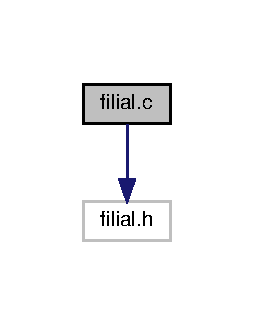
\includegraphics[width=122pt]{filial_8c__incl}
\end{center}
\end{figure}
\subsection*{Estruturas de Dados}
\begin{DoxyCompactItemize}
\item 
struct \hyperlink{structfilial}{filial}
\item 
struct \hyperlink{structcodigoProdutosP}{codigo\+ProdutosP}
\item 
struct \hyperlink{structprodutosPorCliente}{produtos\+Por\+Cliente}
\item 
struct \hyperlink{structcodigoClientes}{codigo\+Clientes}
\end{DoxyCompactItemize}
\subsection*{Funções}
\begin{DoxyCompactItemize}
\item 
ProdP $\ast$ \hyperlink{filial_8c_a8edbe2744a9bab627599f1b7bbd0a23c}{init\+Codigo\+Produto} ()
\begin{DoxyCompactList}\small\item\em Inicialização da estrutura ProdP e da estrutura dados. \end{DoxyCompactList}\item 
void \hyperlink{filial_8c_aa9b7e4c3da81187ae211e029ae7abfb8}{insere\+ClienteP} (Venda $\ast$v, ProdP $\ast$p)
\begin{DoxyCompactList}\small\item\em Insere os dados referentes à struct ProdP. \end{DoxyCompactList}\item 
PpC $\ast$ \hyperlink{filial_8c_a0cb138d733f904c8b89a81c0becda750}{init\+Produto\+Cliente} ()
\begin{DoxyCompactList}\small\item\em Inicializa a estrutura PpC. \end{DoxyCompactList}\item 
void \hyperlink{filial_8c_a0f9d16e5faca61b0081bc8fd43e8f984}{insere\+Produto\+Cliente} (Venda $\ast$v, PpC $\ast$p)
\begin{DoxyCompactList}\small\item\em Insere uma venda na estrutura PpC. \end{DoxyCompactList}\item 
char $\ast$ \hyperlink{filial_8c_af1df915ae2399e2fbbf0b8aab4f81b55}{get\+Nome\+PpC} (PpC $\ast$p)
\begin{DoxyCompactList}\small\item\em Funcao que retorna o nome de um dado PpC. \end{DoxyCompactList}\item 
int \hyperlink{filial_8c_a614abd74004225a52fb5fb43ad07ac33}{get\+Quantidade\+PpC} (PpC $\ast$p, int mes)
\begin{DoxyCompactList}\small\item\em Funcao que retorna a quantidade total de um dado mes. \end{DoxyCompactList}\item 
int \hyperlink{filial_8c_ae7d0235c998eeafc6972fdca030937a5}{get\+Faturacao\+PpC} (PpC $\ast$p, int mes)
\begin{DoxyCompactList}\small\item\em Funcao que retorna a faturacao total de um dado mes. \end{DoxyCompactList}\item 
ClieP $\ast$ \hyperlink{filial_8c_abfa50b3106ed7468daf928e3fede1c03}{init\+Codigo\+Clientes} ()
\begin{DoxyCompactList}\small\item\em Inicialização da estrutura ClieP. \end{DoxyCompactList}\item 
void \hyperlink{filial_8c_a69eb0edc8e3ec7640d317a251ed115c2}{update\+Codigo\+Cliente} (Venda $\ast$v, PpC $\ast$p)
\begin{DoxyCompactList}\small\item\em Atualizacao dos dados da estrutura PpC utilizando uma venda. \end{DoxyCompactList}\item 
void \hyperlink{filial_8c_a92a7bc5d0f5d99498afa909eaffe2ef8}{insere\+Codigo\+Cliente} (Venda $\ast$v, ClieP $\ast$c)
\begin{DoxyCompactList}\small\item\em Funcao que insere os dados uma venda numa estrutura ClieP. \end{DoxyCompactList}\item 
int \hyperlink{filial_8c_a5fc5839f7bc4f8514af51e42e1d14f3d}{get\+Ocupados\+ClieP} (ClieP $\ast$c)
\begin{DoxyCompactList}\small\item\em Funcao que obtem o numero de ocupados da estrutura Pp\+C$\ast$$\ast$ na estrutura ClieP. \end{DoxyCompactList}\item 
int \hyperlink{filial_8c_add54712c6a4b7c3b1119c443443c99b7}{get\+Quantidade\+ClieP} (ClieP $\ast$c, int mes)
\begin{DoxyCompactList}\small\item\em Funcao que obtem a quantidade total de produtos comprados num dado mes de um dado cliente. \end{DoxyCompactList}\item 
PpC $\ast$ \hyperlink{filial_8c_aa975b8bb76ccf055ec06abf0a10b43d2}{get\+Pp\+C\+ClieP} (ClieP $\ast$c, int i)
\begin{DoxyCompactList}\small\item\em Funcao que obtem uma estrutura PpC a partir de uma estrutura ClieP. \end{DoxyCompactList}\item 
Filial $\ast$ \hyperlink{filial_8c_a5727000000ceab10ee0e17bcad54b96e}{init\+Filial} ()
\begin{DoxyCompactList}\small\item\em Funcao que inicializa uma estrutura Filial. \end{DoxyCompactList}\item 
Filial $\ast$ \hyperlink{filial_8c_a6b81df6ede58686e2c36a56486cd56e4}{insere\+Filial} (Filial $\ast$f, Venda $\ast$v)
\begin{DoxyCompactList}\small\item\em Funcao que insere todos os valores da estrutura filial dada uma venda. \end{DoxyCompactList}\item 
int \hyperlink{filial_8c_ae174c41861edf4c914c7af7ad1d47c90}{get\+Quant\+Prod\+Mes\+Cliente} (A\+VL $\ast$f, char $\ast$cliente, int mes)
\begin{DoxyCompactList}\small\item\em Obtem a quantidade de produtos comprados dado o cliente e o mês. \end{DoxyCompactList}\item 
Dados $\ast$ \hyperlink{filial_8c_a0922d9ad281ff82fb29d30ef315e40a4}{get\+Codigos\+ClientsN} (A\+VL $\ast$f, char $\ast$product\+ID)
\begin{DoxyCompactList}\small\item\em Obtem os clientes que compraram o produto correspondente ao codigo dado em promoção tipo N. \end{DoxyCompactList}\item 
Dados $\ast$ \hyperlink{filial_8c_ac5196dc8257c2d5205b5e9b8361da483}{get\+Codigos\+ClientsP} (A\+VL $\ast$f, char $\ast$product\+ID)
\begin{DoxyCompactList}\small\item\em Obtem os clientes que compraram o produto correspondente ao codigo dado em promoção tipo P. \end{DoxyCompactList}\item 
A\+VL $\ast$ \hyperlink{filial_8c_a3ee1ffa99747304fdf7aa19e1ff58ad5}{get\+A\+V\+L\+Produtos} (Filial $\ast$f)
\begin{DoxyCompactList}\small\item\em Funcao que obtem a A\+VL de produtos. \end{DoxyCompactList}\item 
A\+VL $\ast$ \hyperlink{filial_8c_a33d812a6f723a8fe3db03a2dc8c73110}{get\+A\+V\+L\+Clientes} (Filial $\ast$f)
\begin{DoxyCompactList}\small\item\em Funcao que obtem a A\+VL de cliente. \end{DoxyCompactList}\item 
void \hyperlink{filial_8c_a43e361699bd8afee43475f3cb2159368}{free\+ProdP} (ProdP $\ast$p)
\begin{DoxyCompactList}\small\item\em Desaloca a memoria ocupada pela estrutura ProdP. \end{DoxyCompactList}\item 
void \hyperlink{filial_8c_aca09ee09defcd1dfd7c5e1099d2b8807}{free\+A\+V\+LP} (A\+VL $\ast$f)
\begin{DoxyCompactList}\small\item\em Desaloca a memoria ocupada pela estrutura A\+VL. \end{DoxyCompactList}\item 
void \hyperlink{filial_8c_a6361cfa298f0cd36d4d66eb40c28f427}{free\+PpC} (ClieP $\ast$c)
\begin{DoxyCompactList}\small\item\em Desaloca a memoria ocupada pela estrutura PpC. \end{DoxyCompactList}\item 
void \hyperlink{filial_8c_ae738b3104b8b457dd80fc1b67d3a8cd4}{free\+A\+V\+LC} (A\+VL $\ast$f)
\begin{DoxyCompactList}\small\item\em Desaloca a memoria ocupada pela estrutura A\+VL. \end{DoxyCompactList}\item 
void \hyperlink{filial_8c_aadf0ae17a6136cdf1ad1c73dc469dbcf}{free\+Filial} (Filial $\ast$f)
\begin{DoxyCompactList}\small\item\em Desaloca a memória ocupada pelos estrutura Filial. \end{DoxyCompactList}\end{DoxyCompactItemize}


\subsection{Descrição detalhada}
Modulo filial Que inicializa e controi a estrutura. 



\subsection{Documentação das funções}
\mbox{\Hypertarget{filial_8c_ae738b3104b8b457dd80fc1b67d3a8cd4}\label{filial_8c_ae738b3104b8b457dd80fc1b67d3a8cd4}} 
\index{filial.\+c@{filial.\+c}!free\+A\+V\+LC@{free\+A\+V\+LC}}
\index{free\+A\+V\+LC@{free\+A\+V\+LC}!filial.\+c@{filial.\+c}}
\subsubsection{\texorpdfstring{free\+A\+V\+L\+C()}{freeAVLC()}}
{\footnotesize\ttfamily void free\+A\+V\+LC (\begin{DoxyParamCaption}\item[{A\+VL $\ast$}]{f }\end{DoxyParamCaption})}



Desaloca a memoria ocupada pela estrutura A\+VL. 


\begin{DoxyParams}{Parâmetros}
{\em \mbox{[}f\mbox{]}} & Estrutura A\+VL \\
\hline
\end{DoxyParams}


Definido na linha 386 do ficheiro filial.\+c.


\begin{DoxyCode}
386                       \{
387   \textcolor{keywordflow}{if}(f)\{
388     free(\hyperlink{tree_8c_af043329377f4d9303267455cd353fd83}{getKey}(f));
389     \hyperlink{filial_8c_ae738b3104b8b457dd80fc1b67d3a8cd4}{freeAVLC}(\hyperlink{tree_8c_a055813fad18fbe1331c4568fbb9b53ca}{getLeft}(f));
390     \hyperlink{filial_8c_ae738b3104b8b457dd80fc1b67d3a8cd4}{freeAVLC}(\hyperlink{tree_8c_aa92a92ff16f40e2381b0452982b620b3}{getRight}(f));
391     \hyperlink{filial_8c_a6361cfa298f0cd36d4d66eb40c28f427}{freePpC}((ClieP*)(\hyperlink{tree_8c_a1c2789a702672b4fb99d2c622181f949}{getEquals}(f)));
392     free(f);
393     f = NULL;
394   \}
395 \}
\end{DoxyCode}
\mbox{\Hypertarget{filial_8c_aca09ee09defcd1dfd7c5e1099d2b8807}\label{filial_8c_aca09ee09defcd1dfd7c5e1099d2b8807}} 
\index{filial.\+c@{filial.\+c}!free\+A\+V\+LP@{free\+A\+V\+LP}}
\index{free\+A\+V\+LP@{free\+A\+V\+LP}!filial.\+c@{filial.\+c}}
\subsubsection{\texorpdfstring{free\+A\+V\+L\+P()}{freeAVLP()}}
{\footnotesize\ttfamily void free\+A\+V\+LP (\begin{DoxyParamCaption}\item[{A\+VL $\ast$}]{f }\end{DoxyParamCaption})}



Desaloca a memoria ocupada pela estrutura A\+VL. 


\begin{DoxyParams}{Parâmetros}
{\em \mbox{[}f\mbox{]}} & Estrutura A\+VL \\
\hline
\end{DoxyParams}


Definido na linha 353 do ficheiro filial.\+c.


\begin{DoxyCode}
353                       \{
354   \textcolor{keywordflow}{if}(f)\{
355     free(\hyperlink{tree_8c_af043329377f4d9303267455cd353fd83}{getKey}(f));
356     \hyperlink{filial_8c_aca09ee09defcd1dfd7c5e1099d2b8807}{freeAVLP}(\hyperlink{tree_8c_a055813fad18fbe1331c4568fbb9b53ca}{getLeft}(f));
357     \hyperlink{filial_8c_aca09ee09defcd1dfd7c5e1099d2b8807}{freeAVLP}(\hyperlink{tree_8c_aa92a92ff16f40e2381b0452982b620b3}{getRight}(f));
358     \hyperlink{filial_8c_a43e361699bd8afee43475f3cb2159368}{freeProdP}((ProdP*)(\hyperlink{tree_8c_a1c2789a702672b4fb99d2c622181f949}{getEquals}(f)));
359     free(f);
360     f = NULL;
361   \}
362 \}
\end{DoxyCode}
\mbox{\Hypertarget{filial_8c_aadf0ae17a6136cdf1ad1c73dc469dbcf}\label{filial_8c_aadf0ae17a6136cdf1ad1c73dc469dbcf}} 
\index{filial.\+c@{filial.\+c}!free\+Filial@{free\+Filial}}
\index{free\+Filial@{free\+Filial}!filial.\+c@{filial.\+c}}
\subsubsection{\texorpdfstring{free\+Filial()}{freeFilial()}}
{\footnotesize\ttfamily void free\+Filial (\begin{DoxyParamCaption}\item[{Filial $\ast$}]{f }\end{DoxyParamCaption})}



Desaloca a memória ocupada pelos estrutura Filial. 


\begin{DoxyParams}{Parâmetros}
{\em \mbox{[}f\mbox{]}} & Estrutura Filial \\
\hline
\end{DoxyParams}


Definido na linha 403 do ficheiro filial.\+c.


\begin{DoxyCode}
403                           \{
404   \hyperlink{filial_8c_aca09ee09defcd1dfd7c5e1099d2b8807}{freeAVLP}(f->produtos);
405   \hyperlink{filial_8c_ae738b3104b8b457dd80fc1b67d3a8cd4}{freeAVLC}(f->clientes);
406   free(f);
407   f = NULL;
408 \}
\end{DoxyCode}
\mbox{\Hypertarget{filial_8c_a6361cfa298f0cd36d4d66eb40c28f427}\label{filial_8c_a6361cfa298f0cd36d4d66eb40c28f427}} 
\index{filial.\+c@{filial.\+c}!free\+PpC@{free\+PpC}}
\index{free\+PpC@{free\+PpC}!filial.\+c@{filial.\+c}}
\subsubsection{\texorpdfstring{free\+Pp\+C()}{freePpC()}}
{\footnotesize\ttfamily void free\+PpC (\begin{DoxyParamCaption}\item[{ClieP $\ast$}]{c }\end{DoxyParamCaption})}



Desaloca a memoria ocupada pela estrutura PpC. 


\begin{DoxyParams}{Parâmetros}
{\em \mbox{[}p\mbox{]}} & Estrutura PpC \\
\hline
\end{DoxyParams}


Definido na linha 371 do ficheiro filial.\+c.


\begin{DoxyCode}
371                       \{
372   \textcolor{keywordtype}{int} i;
373   \textcolor{keywordflow}{for}(i=0; i < c->ocupados; i++)\{
374     free(c->produtosPorCliente[i]->nome);
375     free(c->produtosPorCliente[i]);
376   \}
377   free(c->produtosPorCliente);
378   free(c);
379 \}
\end{DoxyCode}
\mbox{\Hypertarget{filial_8c_a43e361699bd8afee43475f3cb2159368}\label{filial_8c_a43e361699bd8afee43475f3cb2159368}} 
\index{filial.\+c@{filial.\+c}!free\+ProdP@{free\+ProdP}}
\index{free\+ProdP@{free\+ProdP}!filial.\+c@{filial.\+c}}
\subsubsection{\texorpdfstring{free\+Prod\+P()}{freeProdP()}}
{\footnotesize\ttfamily void free\+ProdP (\begin{DoxyParamCaption}\item[{ProdP $\ast$}]{p }\end{DoxyParamCaption})}



Desaloca a memoria ocupada pela estrutura ProdP. 


\begin{DoxyParams}{Parâmetros}
{\em \mbox{[}p\mbox{]}} & Estrutura ProdP \\
\hline
\end{DoxyParams}


Definido na linha 343 do ficheiro filial.\+c.


\begin{DoxyCode}
343                          \{
344   \hyperlink{clientes_8c_ab0e31c59339ab5320753ed2e47b91a86}{freeDados}((Dados*) p->clienteN);
345   \hyperlink{clientes_8c_ab0e31c59339ab5320753ed2e47b91a86}{freeDados}((Dados*) p->clienteP);
346   free(p);
347 \}
\end{DoxyCode}
\mbox{\Hypertarget{filial_8c_a33d812a6f723a8fe3db03a2dc8c73110}\label{filial_8c_a33d812a6f723a8fe3db03a2dc8c73110}} 
\index{filial.\+c@{filial.\+c}!get\+A\+V\+L\+Clientes@{get\+A\+V\+L\+Clientes}}
\index{get\+A\+V\+L\+Clientes@{get\+A\+V\+L\+Clientes}!filial.\+c@{filial.\+c}}
\subsubsection{\texorpdfstring{get\+A\+V\+L\+Clientes()}{getAVLClientes()}}
{\footnotesize\ttfamily A\+VL$\ast$ get\+A\+V\+L\+Clientes (\begin{DoxyParamCaption}\item[{Filial $\ast$}]{f }\end{DoxyParamCaption})}



Funcao que obtem a A\+VL de cliente. 


\begin{DoxyParams}{Parâmetros}
{\em \mbox{[}f\mbox{]}} & Filial onde vamos buscar a A\+VL cliente \\
\hline
\end{DoxyParams}
\begin{DoxyReturn}{Retorna}
Retorna a A\+VL cliente; 
\end{DoxyReturn}


Definido na linha 335 do ficheiro filial.\+c.


\begin{DoxyCode}
335                                \{
336   \textcolor{keywordflow}{return} f->clientes;
337 \}
\end{DoxyCode}
\mbox{\Hypertarget{filial_8c_a3ee1ffa99747304fdf7aa19e1ff58ad5}\label{filial_8c_a3ee1ffa99747304fdf7aa19e1ff58ad5}} 
\index{filial.\+c@{filial.\+c}!get\+A\+V\+L\+Produtos@{get\+A\+V\+L\+Produtos}}
\index{get\+A\+V\+L\+Produtos@{get\+A\+V\+L\+Produtos}!filial.\+c@{filial.\+c}}
\subsubsection{\texorpdfstring{get\+A\+V\+L\+Produtos()}{getAVLProdutos()}}
{\footnotesize\ttfamily A\+VL$\ast$ get\+A\+V\+L\+Produtos (\begin{DoxyParamCaption}\item[{Filial $\ast$}]{f }\end{DoxyParamCaption})}



Funcao que obtem a A\+VL de produtos. 


\begin{DoxyParams}{Parâmetros}
{\em \mbox{[}f\mbox{]}} & Filial onde vamos buscar a A\+VL produtos \\
\hline
\end{DoxyParams}
\begin{DoxyReturn}{Retorna}
Retorna a A\+VL produtos; 
\end{DoxyReturn}


Definido na linha 326 do ficheiro filial.\+c.


\begin{DoxyCode}
326                                \{
327   \textcolor{keywordflow}{return} f->produtos;
328 \}
\end{DoxyCode}
\mbox{\Hypertarget{filial_8c_a0922d9ad281ff82fb29d30ef315e40a4}\label{filial_8c_a0922d9ad281ff82fb29d30ef315e40a4}} 
\index{filial.\+c@{filial.\+c}!get\+Codigos\+ClientsN@{get\+Codigos\+ClientsN}}
\index{get\+Codigos\+ClientsN@{get\+Codigos\+ClientsN}!filial.\+c@{filial.\+c}}
\subsubsection{\texorpdfstring{get\+Codigos\+Clients\+N()}{getCodigosClientsN()}}
{\footnotesize\ttfamily Dados$\ast$ get\+Codigos\+ClientsN (\begin{DoxyParamCaption}\item[{A\+VL $\ast$}]{f,  }\item[{char $\ast$}]{product\+ID }\end{DoxyParamCaption})}



Obtem os clientes que compraram o produto correspondente ao codigo dado em promoção tipo N. 


\begin{DoxyParams}{Parâmetros}
{\em \mbox{[}f\mbox{]}} & Estrutura A\+VL onde vai ser procurado o produtos \\
\hline
{\em \mbox{[}product\+I\+D\mbox{]}} & Produto que queremos encontrar \\
\hline
\end{DoxyParams}
\begin{DoxyReturn}{Retorna}
Retorna a estrutura dados clienteN 
\end{DoxyReturn}


Definido na linha 282 do ficheiro filial.\+c.


\begin{DoxyCode}
282                                                  \{
283   \textcolor{keywordflow}{if}(\hyperlink{tree_8c_a56e7dddb3c67ac22f3373a010c1c9e21}{searchAVL}(f,productID))\{
284     AVL* tmp = f;
285     \textcolor{keywordflow}{while}(strcmp(\hyperlink{tree_8c_af043329377f4d9303267455cd353fd83}{getKey}(tmp),productID)!= 0)\{
286       \textcolor{keywordflow}{if}(strcmp(\hyperlink{tree_8c_af043329377f4d9303267455cd353fd83}{getKey}(tmp),productID) > 0)\{
287         tmp = \hyperlink{tree_8c_a055813fad18fbe1331c4568fbb9b53ca}{getLeft}(tmp);
288       \}
289       \textcolor{keywordflow}{else}\{
290         tmp = \hyperlink{tree_8c_aa92a92ff16f40e2381b0452982b620b3}{getRight}(tmp);
291       \}
292     \}
293 
294     \textcolor{keywordflow}{return} ((ProdP*)\hyperlink{tree_8c_a1c2789a702672b4fb99d2c622181f949}{getEquals}(tmp))->clienteN;
295   \}
296   \textcolor{keywordflow}{return} NULL;
297 \}
\end{DoxyCode}
\mbox{\Hypertarget{filial_8c_ac5196dc8257c2d5205b5e9b8361da483}\label{filial_8c_ac5196dc8257c2d5205b5e9b8361da483}} 
\index{filial.\+c@{filial.\+c}!get\+Codigos\+ClientsP@{get\+Codigos\+ClientsP}}
\index{get\+Codigos\+ClientsP@{get\+Codigos\+ClientsP}!filial.\+c@{filial.\+c}}
\subsubsection{\texorpdfstring{get\+Codigos\+Clients\+P()}{getCodigosClientsP()}}
{\footnotesize\ttfamily Dados$\ast$ get\+Codigos\+ClientsP (\begin{DoxyParamCaption}\item[{A\+VL $\ast$}]{f,  }\item[{char $\ast$}]{product\+ID }\end{DoxyParamCaption})}



Obtem os clientes que compraram o produto correspondente ao codigo dado em promoção tipo P. 


\begin{DoxyParams}{Parâmetros}
{\em \mbox{[}f\mbox{]}} & Estrutura A\+VL onde vai ser procurado o produtos \\
\hline
{\em \mbox{[}product\+I\+D\mbox{]}} & Produto que queremos encontrar \\
\hline
\end{DoxyParams}
\begin{DoxyReturn}{Retorna}
Retorna a estrutura dados clienteP 
\end{DoxyReturn}


Definido na linha 305 do ficheiro filial.\+c.


\begin{DoxyCode}
305                                                  \{
306   \textcolor{keywordflow}{if}(\hyperlink{tree_8c_a56e7dddb3c67ac22f3373a010c1c9e21}{searchAVL}(f,productID))\{
307     AVL* tmp = f;
308     \textcolor{keywordflow}{while}(strcmp(\hyperlink{tree_8c_af043329377f4d9303267455cd353fd83}{getKey}(tmp),productID)!= 0)\{
309       \textcolor{keywordflow}{if}(strcmp(\hyperlink{tree_8c_af043329377f4d9303267455cd353fd83}{getKey}(tmp),productID) > 0)\{
310         tmp = \hyperlink{tree_8c_a055813fad18fbe1331c4568fbb9b53ca}{getLeft}(tmp);
311       \}
312       \textcolor{keywordflow}{else}\{
313         tmp = \hyperlink{tree_8c_aa92a92ff16f40e2381b0452982b620b3}{getRight}(tmp);
314       \}
315     \}
316     \textcolor{keywordflow}{return} ((ProdP*)\hyperlink{tree_8c_a1c2789a702672b4fb99d2c622181f949}{getEquals}(tmp))->clienteP;
317   \}
318   \textcolor{keywordflow}{return} NULL;
319 \}
\end{DoxyCode}
\mbox{\Hypertarget{filial_8c_ae7d0235c998eeafc6972fdca030937a5}\label{filial_8c_ae7d0235c998eeafc6972fdca030937a5}} 
\index{filial.\+c@{filial.\+c}!get\+Faturacao\+PpC@{get\+Faturacao\+PpC}}
\index{get\+Faturacao\+PpC@{get\+Faturacao\+PpC}!filial.\+c@{filial.\+c}}
\subsubsection{\texorpdfstring{get\+Faturacao\+Pp\+C()}{getFaturacaoPpC()}}
{\footnotesize\ttfamily int get\+Faturacao\+PpC (\begin{DoxyParamCaption}\item[{PpC $\ast$}]{p,  }\item[{int}]{mes }\end{DoxyParamCaption})}



Funcao que retorna a faturacao total de um dado mes. 


\begin{DoxyParams}{Parâmetros}
{\em \mbox{[}p\mbox{]}} & Estrutura PpC \\
\hline
{\em \mbox{[}mes\mbox{]}} & Mes que queremos saber a faturacao \\
\hline
\end{DoxyParams}
\begin{DoxyReturn}{Retorna}
Retorna a faturacao de um dado mes da estrutura PpC 
\end{DoxyReturn}


Definido na linha 115 do ficheiro filial.\+c.


\begin{DoxyCode}
115                                     \{
116   \textcolor{keywordflow}{return} p->fat[mes];
117 \}
\end{DoxyCode}
\mbox{\Hypertarget{filial_8c_af1df915ae2399e2fbbf0b8aab4f81b55}\label{filial_8c_af1df915ae2399e2fbbf0b8aab4f81b55}} 
\index{filial.\+c@{filial.\+c}!get\+Nome\+PpC@{get\+Nome\+PpC}}
\index{get\+Nome\+PpC@{get\+Nome\+PpC}!filial.\+c@{filial.\+c}}
\subsubsection{\texorpdfstring{get\+Nome\+Pp\+C()}{getNomePpC()}}
{\footnotesize\ttfamily char$\ast$ get\+Nome\+PpC (\begin{DoxyParamCaption}\item[{PpC $\ast$}]{p }\end{DoxyParamCaption})}



Funcao que retorna o nome de um dado PpC. 


\begin{DoxyParams}{Parâmetros}
{\em \mbox{[}p\mbox{]}} & Estrutura PpC \\
\hline
\end{DoxyParams}
\begin{DoxyReturn}{Retorna}
Retorna o nome do produto da estrutura PpC 
\end{DoxyReturn}


Definido na linha 95 do ficheiro filial.\+c.


\begin{DoxyCode}
95                          \{
96   \textcolor{keywordflow}{return} strdup(p->nome);
97 \}
\end{DoxyCode}
\mbox{\Hypertarget{filial_8c_a5fc5839f7bc4f8514af51e42e1d14f3d}\label{filial_8c_a5fc5839f7bc4f8514af51e42e1d14f3d}} 
\index{filial.\+c@{filial.\+c}!get\+Ocupados\+ClieP@{get\+Ocupados\+ClieP}}
\index{get\+Ocupados\+ClieP@{get\+Ocupados\+ClieP}!filial.\+c@{filial.\+c}}
\subsubsection{\texorpdfstring{get\+Ocupados\+Clie\+P()}{getOcupadosClieP()}}
{\footnotesize\ttfamily int get\+Ocupados\+ClieP (\begin{DoxyParamCaption}\item[{ClieP $\ast$}]{c }\end{DoxyParamCaption})}



Funcao que obtem o numero de ocupados da estrutura Pp\+C$\ast$$\ast$ na estrutura ClieP. 


\begin{DoxyParams}{Parâmetros}
{\em \mbox{[}c\mbox{]}} & Estrutura ClieP \\
\hline
\end{DoxyParams}
\begin{DoxyReturn}{Retorna}
Retorna o numero de ocupados da estrutura Pp\+C$\ast$$\ast$ 
\end{DoxyReturn}


Definido na linha 175 do ficheiro filial.\+c.


\begin{DoxyCode}
175                               \{
176   \textcolor{keywordflow}{return} c->ocupados;
177 \}
\end{DoxyCode}
\mbox{\Hypertarget{filial_8c_aa975b8bb76ccf055ec06abf0a10b43d2}\label{filial_8c_aa975b8bb76ccf055ec06abf0a10b43d2}} 
\index{filial.\+c@{filial.\+c}!get\+Pp\+C\+ClieP@{get\+Pp\+C\+ClieP}}
\index{get\+Pp\+C\+ClieP@{get\+Pp\+C\+ClieP}!filial.\+c@{filial.\+c}}
\subsubsection{\texorpdfstring{get\+Pp\+C\+Clie\+P()}{getPpCClieP()}}
{\footnotesize\ttfamily PpC$\ast$ get\+Pp\+C\+ClieP (\begin{DoxyParamCaption}\item[{ClieP $\ast$}]{c,  }\item[{int}]{i }\end{DoxyParamCaption})}



Funcao que obtem uma estrutura PpC a partir de uma estrutura ClieP. 


\begin{DoxyParams}{Parâmetros}
{\em \mbox{[}c\mbox{]}} & Estrutura ClieP \\
\hline
{\em \mbox{[}i\mbox{]}} & Indice i onde encontramos a estrutura PpC \\
\hline
\end{DoxyParams}
\begin{DoxyReturn}{Retorna}
Estrutura PpC 
\end{DoxyReturn}


Definido na linha 195 do ficheiro filial.\+c.


\begin{DoxyCode}
195                                 \{
196   \textcolor{keywordflow}{return} c->produtosPorCliente[i];
197 \}
\end{DoxyCode}
\mbox{\Hypertarget{filial_8c_add54712c6a4b7c3b1119c443443c99b7}\label{filial_8c_add54712c6a4b7c3b1119c443443c99b7}} 
\index{filial.\+c@{filial.\+c}!get\+Quantidade\+ClieP@{get\+Quantidade\+ClieP}}
\index{get\+Quantidade\+ClieP@{get\+Quantidade\+ClieP}!filial.\+c@{filial.\+c}}
\subsubsection{\texorpdfstring{get\+Quantidade\+Clie\+P()}{getQuantidadeClieP()}}
{\footnotesize\ttfamily int get\+Quantidade\+ClieP (\begin{DoxyParamCaption}\item[{ClieP $\ast$}]{c,  }\item[{int}]{mes }\end{DoxyParamCaption})}



Funcao que obtem a quantidade total de produtos comprados num dado mes de um dado cliente. 


\begin{DoxyParams}{Parâmetros}
{\em \mbox{[}c\mbox{]}} & Estrutura ClieP \\
\hline
{\em \mbox{[}mes\mbox{]}} & Mes em que quer a quantidade \\
\hline
\end{DoxyParams}
\begin{DoxyReturn}{Retorna}
Quantidade total de produtos comprados num dados mes 
\end{DoxyReturn}


Definido na linha 185 do ficheiro filial.\+c.


\begin{DoxyCode}
185                                           \{
186   \textcolor{keywordflow}{return} c->quant[mes-1];
187 \}
\end{DoxyCode}
\mbox{\Hypertarget{filial_8c_a614abd74004225a52fb5fb43ad07ac33}\label{filial_8c_a614abd74004225a52fb5fb43ad07ac33}} 
\index{filial.\+c@{filial.\+c}!get\+Quantidade\+PpC@{get\+Quantidade\+PpC}}
\index{get\+Quantidade\+PpC@{get\+Quantidade\+PpC}!filial.\+c@{filial.\+c}}
\subsubsection{\texorpdfstring{get\+Quantidade\+Pp\+C()}{getQuantidadePpC()}}
{\footnotesize\ttfamily int get\+Quantidade\+PpC (\begin{DoxyParamCaption}\item[{PpC $\ast$}]{p,  }\item[{int}]{mes }\end{DoxyParamCaption})}



Funcao que retorna a quantidade total de um dado mes. 


\begin{DoxyParams}{Parâmetros}
{\em \mbox{[}p\mbox{]}} & Estrutura PpC \\
\hline
{\em \mbox{[}mes\mbox{]}} & Mes que queremos saber a quantidade \\
\hline
\end{DoxyParams}
\begin{DoxyReturn}{Retorna}
Retorna a quantidade de um dado mes da estrutura PpC 
\end{DoxyReturn}


Definido na linha 105 do ficheiro filial.\+c.


\begin{DoxyCode}
105                                      \{
106   \textcolor{keywordflow}{return} p->quant[mes];
107 \}
\end{DoxyCode}
\mbox{\Hypertarget{filial_8c_ae174c41861edf4c914c7af7ad1d47c90}\label{filial_8c_ae174c41861edf4c914c7af7ad1d47c90}} 
\index{filial.\+c@{filial.\+c}!get\+Quant\+Prod\+Mes\+Cliente@{get\+Quant\+Prod\+Mes\+Cliente}}
\index{get\+Quant\+Prod\+Mes\+Cliente@{get\+Quant\+Prod\+Mes\+Cliente}!filial.\+c@{filial.\+c}}
\subsubsection{\texorpdfstring{get\+Quant\+Prod\+Mes\+Cliente()}{getQuantProdMesCliente()}}
{\footnotesize\ttfamily int get\+Quant\+Prod\+Mes\+Cliente (\begin{DoxyParamCaption}\item[{A\+VL $\ast$}]{f,  }\item[{char $\ast$}]{cliente,  }\item[{int}]{mes }\end{DoxyParamCaption})}



Obtem a quantidade de produtos comprados dado o cliente e o mês. 


\begin{DoxyParams}{Parâmetros}
{\em \mbox{[}f\mbox{]}} & Estrutura avl onde vai ser procurado o cliente \\
\hline
{\em \mbox{[}cliente\mbox{]}} & Cliente que queremos encontrar \\
\hline
{\em \mbox{[}mes\mbox{]}} & Mes que o utilizador deseja informacoes \\
\hline
\end{DoxyParams}
\begin{DoxyReturn}{Retorna}
Retorna a quantidade de produtos comprados 
\end{DoxyReturn}


Definido na linha 262 do ficheiro filial.\+c.


\begin{DoxyCode}
262                                                          \{
263   \textcolor{keywordflow}{if}(\hyperlink{tree_8c_a56e7dddb3c67ac22f3373a010c1c9e21}{searchAVL}(f,cliente))\{
264     AVL* aux = f;
265     \textcolor{keywordflow}{while}(strcmp(\hyperlink{tree_8c_af043329377f4d9303267455cd353fd83}{getKey}(aux),cliente)!= 0)\{
266       \textcolor{keywordflow}{if}(strcmp(\hyperlink{tree_8c_af043329377f4d9303267455cd353fd83}{getKey}(aux),cliente) > 0)
267         aux = \hyperlink{tree_8c_a055813fad18fbe1331c4568fbb9b53ca}{getLeft}(aux);
268       \textcolor{keywordflow}{else}
269         aux = \hyperlink{tree_8c_aa92a92ff16f40e2381b0452982b620b3}{getRight}(aux);
270     \}
271     \textcolor{keywordflow}{return} ((ClieP*)\hyperlink{tree_8c_a1c2789a702672b4fb99d2c622181f949}{getEquals}(aux))->quant[mes];
272   \}
273   \textcolor{keywordflow}{return} 0;
274 \}
\end{DoxyCode}
\mbox{\Hypertarget{filial_8c_abfa50b3106ed7468daf928e3fede1c03}\label{filial_8c_abfa50b3106ed7468daf928e3fede1c03}} 
\index{filial.\+c@{filial.\+c}!init\+Codigo\+Clientes@{init\+Codigo\+Clientes}}
\index{init\+Codigo\+Clientes@{init\+Codigo\+Clientes}!filial.\+c@{filial.\+c}}
\subsubsection{\texorpdfstring{init\+Codigo\+Clientes()}{initCodigoClientes()}}
{\footnotesize\ttfamily ClieP$\ast$ init\+Codigo\+Clientes (\begin{DoxyParamCaption}{ }\end{DoxyParamCaption})}



Inicialização da estrutura ClieP. 

\begin{DoxyReturn}{Retorna}
Estrutura inicializada ClieP 
\end{DoxyReturn}


Definido na linha 124 do ficheiro filial.\+c.


\begin{DoxyCode}
124                             \{
125   ClieP* c = malloc(\textcolor{keyword}{sizeof}(ClieP));
126   c->ocupados = 0;
127   \textcolor{keywordtype}{int} i;
128   \textcolor{keywordflow}{for}(i = 0; i < 12; i++)\{
129     c->quant[i] = 0;
130   \}
131   c->produtosPorCliente = NULL;
132   \textcolor{keywordflow}{return} c;
133 \}
\end{DoxyCode}
\mbox{\Hypertarget{filial_8c_a8edbe2744a9bab627599f1b7bbd0a23c}\label{filial_8c_a8edbe2744a9bab627599f1b7bbd0a23c}} 
\index{filial.\+c@{filial.\+c}!init\+Codigo\+Produto@{init\+Codigo\+Produto}}
\index{init\+Codigo\+Produto@{init\+Codigo\+Produto}!filial.\+c@{filial.\+c}}
\subsubsection{\texorpdfstring{init\+Codigo\+Produto()}{initCodigoProduto()}}
{\footnotesize\ttfamily ProdP$\ast$ init\+Codigo\+Produto (\begin{DoxyParamCaption}{ }\end{DoxyParamCaption})}



Inicialização da estrutura ProdP e da estrutura dados. 

\begin{DoxyReturn}{Retorna}
Retorna a nova estrutura ProdP 
\end{DoxyReturn}


Definido na linha 35 do ficheiro filial.\+c.


\begin{DoxyCode}
35                            \{
36   ProdP* p = malloc(\textcolor{keyword}{sizeof}(ProdP));
37   p->clienteN = \hyperlink{clientes_8c_ab5e7eab04f090f920f5ea98c6cb1a505}{initDados}();
38   p->clienteP = \hyperlink{clientes_8c_ab5e7eab04f090f920f5ea98c6cb1a505}{initDados}();
39   \textcolor{keywordflow}{return} p;
40 \}
\end{DoxyCode}
\mbox{\Hypertarget{filial_8c_a5727000000ceab10ee0e17bcad54b96e}\label{filial_8c_a5727000000ceab10ee0e17bcad54b96e}} 
\index{filial.\+c@{filial.\+c}!init\+Filial@{init\+Filial}}
\index{init\+Filial@{init\+Filial}!filial.\+c@{filial.\+c}}
\subsubsection{\texorpdfstring{init\+Filial()}{initFilial()}}
{\footnotesize\ttfamily Filial$\ast$ init\+Filial (\begin{DoxyParamCaption}{ }\end{DoxyParamCaption})}



Funcao que inicializa uma estrutura Filial. 

\begin{DoxyReturn}{Retorna}
Retorna a estrutura Filial inicializada 
\end{DoxyReturn}


Definido na linha 203 do ficheiro filial.\+c.


\begin{DoxyCode}
203                     \{
204   Filial* f = malloc(\textcolor{keyword}{sizeof}(Filial));
205   f->produtos = NULL;
206   f->clientes = NULL;
207   \textcolor{keywordflow}{return} f;
208 \}
\end{DoxyCode}
\mbox{\Hypertarget{filial_8c_a0cb138d733f904c8b89a81c0becda750}\label{filial_8c_a0cb138d733f904c8b89a81c0becda750}} 
\index{filial.\+c@{filial.\+c}!init\+Produto\+Cliente@{init\+Produto\+Cliente}}
\index{init\+Produto\+Cliente@{init\+Produto\+Cliente}!filial.\+c@{filial.\+c}}
\subsubsection{\texorpdfstring{init\+Produto\+Cliente()}{initProdutoCliente()}}
{\footnotesize\ttfamily PpC$\ast$ init\+Produto\+Cliente (\begin{DoxyParamCaption}{ }\end{DoxyParamCaption})}



Inicializa a estrutura PpC. 

\begin{DoxyReturn}{Retorna}
Estrutura PpC inicializada 
\end{DoxyReturn}


Definido na linha 66 do ficheiro filial.\+c.


\begin{DoxyCode}
66                           \{
67   \textcolor{keywordtype}{int} i;
68   PpC* p = malloc(\textcolor{keyword}{sizeof}(PpC));
69   p->nome = NULL;
70   \textcolor{keywordflow}{for}(i = 0; i < 12; i++)\{
71     p->quant[i] = 0;
72   \}
73   \textcolor{keywordflow}{for}(i = 0; i < 12; i++)\{
74     p->fat[i] = 0;
75   \}
76   \textcolor{keywordflow}{return} p;
77 \}
\end{DoxyCode}
\mbox{\Hypertarget{filial_8c_aa9b7e4c3da81187ae211e029ae7abfb8}\label{filial_8c_aa9b7e4c3da81187ae211e029ae7abfb8}} 
\index{filial.\+c@{filial.\+c}!insere\+ClienteP@{insere\+ClienteP}}
\index{insere\+ClienteP@{insere\+ClienteP}!filial.\+c@{filial.\+c}}
\subsubsection{\texorpdfstring{insere\+Cliente\+P()}{insereClienteP()}}
{\footnotesize\ttfamily void insere\+ClienteP (\begin{DoxyParamCaption}\item[{Venda $\ast$}]{v,  }\item[{ProdP $\ast$}]{p }\end{DoxyParamCaption})}



Insere os dados referentes à struct ProdP. 


\begin{DoxyParams}{Parâmetros}
{\em \mbox{[}v\mbox{]}} & Venda utilizada para inserir o cliente \\
\hline
{\em \mbox{[}p\mbox{]}} & Estrutura ProdP onde vai ser inserida o cliente \\
\hline
\end{DoxyParams}


Definido na linha 47 do ficheiro filial.\+c.


\begin{DoxyCode}
47                                        \{
48   \textcolor{keywordflow}{if}(\hyperlink{vendas_8c_ac48ab849f5af46f09394a208f41029e6}{getPromocao}(v) == \textcolor{charliteral}{'N'})\{
49     \textcolor{keywordflow}{if}(p->clienteN->size == p->clienteN->ocupados)\{
50       \hyperlink{clientes_8c_ab93f3f48a62ea57a21aa91347dc699c7}{reallocDados}(p->clienteN);
51     \}
52     p->clienteN->str[p->clienteN->ocupados++] = \hyperlink{vendas_8c_a6a66082eb395bd8876be3504c51aa264}{getCliente}(v);
53   \}
54   \textcolor{keywordflow}{else} \{
55     \textcolor{keywordflow}{if}(p->clienteP->size == p->clienteP->ocupados)\{
56       \hyperlink{clientes_8c_ab93f3f48a62ea57a21aa91347dc699c7}{reallocDados}(p->clienteP);
57     \}
58     p->clienteP->str[p->clienteP->ocupados++] = \hyperlink{vendas_8c_a6a66082eb395bd8876be3504c51aa264}{getCliente}(v);
59   \}
60 \}
\end{DoxyCode}
\mbox{\Hypertarget{filial_8c_a92a7bc5d0f5d99498afa909eaffe2ef8}\label{filial_8c_a92a7bc5d0f5d99498afa909eaffe2ef8}} 
\index{filial.\+c@{filial.\+c}!insere\+Codigo\+Cliente@{insere\+Codigo\+Cliente}}
\index{insere\+Codigo\+Cliente@{insere\+Codigo\+Cliente}!filial.\+c@{filial.\+c}}
\subsubsection{\texorpdfstring{insere\+Codigo\+Cliente()}{insereCodigoCliente()}}
{\footnotesize\ttfamily void insere\+Codigo\+Cliente (\begin{DoxyParamCaption}\item[{Venda $\ast$}]{v,  }\item[{ClieP $\ast$}]{c }\end{DoxyParamCaption})}



Funcao que insere os dados uma venda numa estrutura ClieP. 


\begin{DoxyParams}{Parâmetros}
{\em \mbox{[}v\mbox{]}} & Venda utilizada para obter os dados \\
\hline
{\em \mbox{[}c\mbox{]}} & Estrutura onde vão ser inseridos os dados \\
\hline
\end{DoxyParams}


Definido na linha 151 do ficheiro filial.\+c.


\begin{DoxyCode}
151                                             \{
152 
153   PpC** aux = c->produtosPorCliente;
154   \textcolor{keywordtype}{int} i = 0;
155   \textcolor{keywordtype}{char}* prod = \hyperlink{vendas_8c_a44aa4bbfb64f14bb33fefaeb575c00e1}{getProduto}(v);
156   \textcolor{keywordflow}{while}(i < c->ocupados && (strcmp(aux[i]->nome,prod) != 0)) i++;
157   \textcolor{keywordflow}{if}(i == c->ocupados)\{
158     \textcolor{keywordtype}{int} size = (i*2)+1;
159     c->produtosPorCliente = realloc(c->produtosPorCliente,size*\textcolor{keyword}{sizeof}(PpC*));
160     c->produtosPorCliente[c->ocupados] = \hyperlink{filial_8c_a0cb138d733f904c8b89a81c0becda750}{initProdutoCliente}();
161     \hyperlink{filial_8c_a0f9d16e5faca61b0081bc8fd43e8f984}{insereProdutoCliente}(v,c->produtosPorCliente[c->ocupados++]);
162     c->quant[\hyperlink{vendas_8c_a1178cf1dea33bcb6c9612d46f7534f33}{getData}(v)-1] += \hyperlink{vendas_8c_ae3196cffdcf5289440c1ee56ed5ee0d7}{getQuantidade}(v);
163   \}
164   \textcolor{keywordflow}{else}\{
165     \hyperlink{filial_8c_a69eb0edc8e3ec7640d317a251ed115c2}{updateCodigoCliente}(v,aux[i]);
166   \}
167   free(prod);
168 \}
\end{DoxyCode}
\mbox{\Hypertarget{filial_8c_a6b81df6ede58686e2c36a56486cd56e4}\label{filial_8c_a6b81df6ede58686e2c36a56486cd56e4}} 
\index{filial.\+c@{filial.\+c}!insere\+Filial@{insere\+Filial}}
\index{insere\+Filial@{insere\+Filial}!filial.\+c@{filial.\+c}}
\subsubsection{\texorpdfstring{insere\+Filial()}{insereFilial()}}
{\footnotesize\ttfamily Filial$\ast$ insere\+Filial (\begin{DoxyParamCaption}\item[{Filial $\ast$}]{f,  }\item[{Venda $\ast$}]{v }\end{DoxyParamCaption})}



Funcao que insere todos os valores da estrutura filial dada uma venda. 


\begin{DoxyParams}{Parâmetros}
{\em \mbox{[}f\mbox{]}} & Filial onde vao ser inseridos os valores de todas as suas estruturas \\
\hline
{\em \mbox{[}v\mbox{]}} & Venda utilizada para obter os dados \\
\hline
\end{DoxyParams}
\begin{DoxyReturn}{Retorna}
Retorna a filial com os dados todos inseridos 
\end{DoxyReturn}


Definido na linha 227 do ficheiro filial.\+c.


\begin{DoxyCode}
227                                         \{
228   \textcolor{keywordtype}{char}* prod = \hyperlink{vendas_8c_a44aa4bbfb64f14bb33fefaeb575c00e1}{getProduto}(v);
229   \textcolor{keywordtype}{char}* cli = \hyperlink{vendas_8c_a6a66082eb395bd8876be3504c51aa264}{getCliente}(v);
230   AVL* ap = searchAVLTMP(f->produtos,prod);
231   \textcolor{keywordflow}{if}(ap != NULL)\{
232     \hyperlink{filial_8c_aa9b7e4c3da81187ae211e029ae7abfb8}{insereClienteP}(v,(ProdP*) \hyperlink{tree_8c_a1c2789a702672b4fb99d2c622181f949}{getEquals}(ap));
233   \}
234   \textcolor{keywordflow}{else}
235   \{
236     ProdP* p = \hyperlink{filial_8c_a8edbe2744a9bab627599f1b7bbd0a23c}{initCodigoProduto}();
237     \hyperlink{filial_8c_aa9b7e4c3da81187ae211e029ae7abfb8}{insereClienteP}(v,p);
238     f->produtos = \hyperlink{tree_8c_a8792d9847f06c27e4955b63f63239305}{insert}(f->produtos,strdup(prod),p);
239   \}
240   AVL* ac = (searchAVLTMP(f->clientes,cli));
241   \textcolor{keywordflow}{if}(ac != NULL)\{
242     \hyperlink{filial_8c_a92a7bc5d0f5d99498afa909eaffe2ef8}{insereCodigoCliente}(v,\hyperlink{tree_8c_a1c2789a702672b4fb99d2c622181f949}{getEquals}(ac));
243   \}
244   \textcolor{keywordflow}{else} \{
245     ClieP* c = \hyperlink{filial_8c_abfa50b3106ed7468daf928e3fede1c03}{initCodigoClientes}();
246     \hyperlink{filial_8c_a92a7bc5d0f5d99498afa909eaffe2ef8}{insereCodigoCliente}(v,c);
247     f->clientes = \hyperlink{tree_8c_a8792d9847f06c27e4955b63f63239305}{insert}(f->clientes,strdup(cli),c);
248   \}
249   free(prod);
250   free(cli);
251   \textcolor{keywordflow}{return} f;
252 \}
\end{DoxyCode}
\mbox{\Hypertarget{filial_8c_a0f9d16e5faca61b0081bc8fd43e8f984}\label{filial_8c_a0f9d16e5faca61b0081bc8fd43e8f984}} 
\index{filial.\+c@{filial.\+c}!insere\+Produto\+Cliente@{insere\+Produto\+Cliente}}
\index{insere\+Produto\+Cliente@{insere\+Produto\+Cliente}!filial.\+c@{filial.\+c}}
\subsubsection{\texorpdfstring{insere\+Produto\+Cliente()}{insereProdutoCliente()}}
{\footnotesize\ttfamily void insere\+Produto\+Cliente (\begin{DoxyParamCaption}\item[{Venda $\ast$}]{v,  }\item[{PpC $\ast$}]{p }\end{DoxyParamCaption})}



Insere uma venda na estrutura PpC. 


\begin{DoxyParams}{Parâmetros}
{\em \mbox{[}v\mbox{]}} & Venda utilizada para inserir os dados na estrutura \\
\hline
{\em \mbox{[}p\mbox{]}} & Estrutura onde vao ser inseridos os dados \\
\hline
\end{DoxyParams}


Definido na linha 84 do ficheiro filial.\+c.


\begin{DoxyCode}
84                                            \{
85   p->nome = \hyperlink{vendas_8c_a44aa4bbfb64f14bb33fefaeb575c00e1}{getProduto}(v);
86   p->quant[\hyperlink{vendas_8c_a1178cf1dea33bcb6c9612d46f7534f33}{getData}(v)-1] += \hyperlink{vendas_8c_ae3196cffdcf5289440c1ee56ed5ee0d7}{getQuantidade}(v);
87   p->fat[\hyperlink{vendas_8c_a1178cf1dea33bcb6c9612d46f7534f33}{getData}(v)-1] += \hyperlink{vendas_8c_a9cde304721e7cf45c51ec95bcf625de4}{getPreco}(v)*\hyperlink{vendas_8c_ae3196cffdcf5289440c1ee56ed5ee0d7}{getQuantidade}(v);
88 \}
\end{DoxyCode}
\mbox{\Hypertarget{filial_8c_a69eb0edc8e3ec7640d317a251ed115c2}\label{filial_8c_a69eb0edc8e3ec7640d317a251ed115c2}} 
\index{filial.\+c@{filial.\+c}!update\+Codigo\+Cliente@{update\+Codigo\+Cliente}}
\index{update\+Codigo\+Cliente@{update\+Codigo\+Cliente}!filial.\+c@{filial.\+c}}
\subsubsection{\texorpdfstring{update\+Codigo\+Cliente()}{updateCodigoCliente()}}
{\footnotesize\ttfamily void update\+Codigo\+Cliente (\begin{DoxyParamCaption}\item[{Venda $\ast$}]{v,  }\item[{PpC $\ast$}]{p }\end{DoxyParamCaption})}



Atualizacao dos dados da estrutura PpC utilizando uma venda. 


\begin{DoxyParams}{Parâmetros}
{\em \mbox{[}v\mbox{]}} & Venda utilizada para atualizar os valores da estrutura PpC \\
\hline
{\em \mbox{[}p\mbox{]}} & Estrutura PpC que vai ser atualizada \\
\hline
\end{DoxyParams}


Definido na linha 141 do ficheiro filial.\+c.


\begin{DoxyCode}
141                                           \{
142   p->quant[\hyperlink{vendas_8c_a1178cf1dea33bcb6c9612d46f7534f33}{getData}(v)-1] += \hyperlink{vendas_8c_ae3196cffdcf5289440c1ee56ed5ee0d7}{getQuantidade}(v);
143   p->fat[\hyperlink{vendas_8c_a1178cf1dea33bcb6c9612d46f7534f33}{getData}(v)-1] += \hyperlink{vendas_8c_a9cde304721e7cf45c51ec95bcf625de4}{getPreco}(v);
144 \}
\end{DoxyCode}

\hypertarget{produtos_8c}{}\section{Referência ao ficheiro produtos.\+c}
\label{produtos_8c}\index{produtos.\+c@{produtos.\+c}}


Ficheiro que contem funções utilizadas para os produtos.  


{\ttfamily \#include \char`\"{}produtos.\+h\char`\"{}}\newline
Diagrama de dependências de inclusão para produtos.\+c\+:
\nopagebreak
\begin{figure}[H]
\begin{center}
\leavevmode
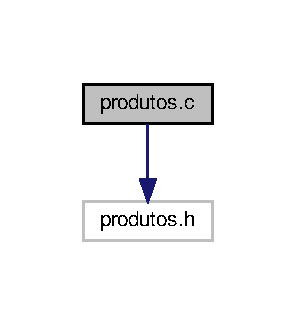
\includegraphics[width=142pt]{produtos_8c__incl}
\end{center}
\end{figure}
\subsection*{Funções}
\begin{DoxyCompactItemize}
\item 
int \hyperlink{produtos_8c_a3fd719b07970fa788d3ad51440484d1e}{valid\+\_\+\+Produtos} (char $\ast$str)
\begin{DoxyCompactList}\small\item\em Valida os produtos. \end{DoxyCompactList}\item 
void \hyperlink{produtos_8c_ac0ee60ad5a3fab414fc2e7470e43e15f}{read\+\_\+\+Produtos} (Dados $\ast$produtos, char $\ast$file\+Path)
\begin{DoxyCompactList}\small\item\em Função que lê um ficheiro .txt com a informacao relativa aos produtos. \end{DoxyCompactList}\item 
int \hyperlink{produtos_8c_a7c722b918c15082ce56ff92ab07a47e5}{get\+OcupadosP} (Dados $\ast$produtos)
\begin{DoxyCompactList}\small\item\em Função que devolve o espaço ocupado pelos produtos na string. \end{DoxyCompactList}\item 
int \hyperlink{produtos_8c_a05943ed85340c50750c61a556ad205b7}{get\+LidasP} (Dados $\ast$produtos)
\begin{DoxyCompactList}\small\item\em Função que devolve os produtos lidos. \end{DoxyCompactList}\item 
char $\ast$ \hyperlink{produtos_8c_a469255f6be632c57839aa91f2e5040d1}{get\+ProdutoP} (int i, Dados $\ast$produtos)
\begin{DoxyCompactList}\small\item\em Função que devolve um array com os produtos. \end{DoxyCompactList}\end{DoxyCompactItemize}


\subsection{Descrição detalhada}
Ficheiro que contem funções utilizadas para os produtos. 



\subsection{Documentação das funções}
\mbox{\Hypertarget{produtos_8c_a05943ed85340c50750c61a556ad205b7}\label{produtos_8c_a05943ed85340c50750c61a556ad205b7}} 
\index{produtos.\+c@{produtos.\+c}!get\+LidasP@{get\+LidasP}}
\index{get\+LidasP@{get\+LidasP}!produtos.\+c@{produtos.\+c}}
\subsubsection{\texorpdfstring{get\+Lidas\+P()}{getLidasP()}}
{\footnotesize\ttfamily int get\+LidasP (\begin{DoxyParamCaption}\item[{Dados $\ast$}]{produtos }\end{DoxyParamCaption})}



Função que devolve os produtos lidos. 


\begin{DoxyParams}{Parâmetros}
{\em \mbox{[}produtos\mbox{]}} & Dados dos produtos \\
\hline
\end{DoxyParams}
\begin{DoxyReturn}{Retorna}
Produtos lidos 
\end{DoxyReturn}


Definido na linha 71 do ficheiro produtos.\+c.


\begin{DoxyCode}
71                                \{
72   \textcolor{keywordflow}{return} produtos->lidas;
73 \}
\end{DoxyCode}
\mbox{\Hypertarget{produtos_8c_a7c722b918c15082ce56ff92ab07a47e5}\label{produtos_8c_a7c722b918c15082ce56ff92ab07a47e5}} 
\index{produtos.\+c@{produtos.\+c}!get\+OcupadosP@{get\+OcupadosP}}
\index{get\+OcupadosP@{get\+OcupadosP}!produtos.\+c@{produtos.\+c}}
\subsubsection{\texorpdfstring{get\+Ocupados\+P()}{getOcupadosP()}}
{\footnotesize\ttfamily int get\+OcupadosP (\begin{DoxyParamCaption}\item[{Dados $\ast$}]{produtos }\end{DoxyParamCaption})}



Função que devolve o espaço ocupado pelos produtos na string. 


\begin{DoxyParams}{Parâmetros}
{\em \mbox{[}produtos\mbox{]}} & Dados dos produtos \\
\hline
\end{DoxyParams}
\begin{DoxyReturn}{Retorna}
Espaço ocupado pelos produtos na string 
\end{DoxyReturn}


Definido na linha 61 do ficheiro produtos.\+c.


\begin{DoxyCode}
61                                   \{
62   \textcolor{keywordflow}{return} produtos->ocupados;
63 \}
\end{DoxyCode}
\mbox{\Hypertarget{produtos_8c_a469255f6be632c57839aa91f2e5040d1}\label{produtos_8c_a469255f6be632c57839aa91f2e5040d1}} 
\index{produtos.\+c@{produtos.\+c}!get\+ProdutoP@{get\+ProdutoP}}
\index{get\+ProdutoP@{get\+ProdutoP}!produtos.\+c@{produtos.\+c}}
\subsubsection{\texorpdfstring{get\+Produto\+P()}{getProdutoP()}}
{\footnotesize\ttfamily char$\ast$ get\+ProdutoP (\begin{DoxyParamCaption}\item[{int}]{i,  }\item[{Dados $\ast$}]{produtos }\end{DoxyParamCaption})}



Função que devolve um array com os produtos. 


\begin{DoxyParams}{Parâmetros}
{\em \mbox{[}i\mbox{]}} & Indíce do array str \\
\hline
{\em \mbox{[}produtos\mbox{]}} & Dados dos produtos \\
\hline
\end{DoxyParams}
\begin{DoxyReturn}{Retorna}
Array com os produtos 
\end{DoxyReturn}


Definido na linha 82 do ficheiro produtos.\+c.


\begin{DoxyCode}
82                                          \{
83   \textcolor{keywordflow}{return} strdup(produtos->str[i]);
84 \}
\end{DoxyCode}
\mbox{\Hypertarget{produtos_8c_ac0ee60ad5a3fab414fc2e7470e43e15f}\label{produtos_8c_ac0ee60ad5a3fab414fc2e7470e43e15f}} 
\index{produtos.\+c@{produtos.\+c}!read\+\_\+\+Produtos@{read\+\_\+\+Produtos}}
\index{read\+\_\+\+Produtos@{read\+\_\+\+Produtos}!produtos.\+c@{produtos.\+c}}
\subsubsection{\texorpdfstring{read\+\_\+\+Produtos()}{read\_Produtos()}}
{\footnotesize\ttfamily void read\+\_\+\+Produtos (\begin{DoxyParamCaption}\item[{Dados $\ast$}]{produtos,  }\item[{char $\ast$}]{file\+Path }\end{DoxyParamCaption})}



Função que lê um ficheiro .txt com a informacao relativa aos produtos. 


\begin{DoxyParams}{Parâmetros}
{\em \mbox{[}produtos\mbox{]}} & Dados dos produtos \\
\hline
{\em \mbox{[}file\+Path\mbox{]}} & Caminho do ficheiro \\
\hline
\end{DoxyParams}


Definido na linha 34 do ficheiro produtos.\+c.


\begin{DoxyCode}
34                                                     \{
35   FILE* f = fopen(filePath, \textcolor{stringliteral}{"r"});
36   \textcolor{keywordflow}{if} (f == NULL)\{
37     printf(\textcolor{stringliteral}{"Ficheiro produtos inexistente\(\backslash\)n"});
38   \}
39   \textcolor{keywordtype}{char} str[1024];
40   \textcolor{keywordflow}{while}(fgets(str,1024,f))\{
41     produtos->lidas++;
42     \textcolor{keywordflow}{if}(\hyperlink{produtos_8c_a3fd719b07970fa788d3ad51440484d1e}{valid\_Produtos}(strtok(str,\textcolor{stringliteral}{"\(\backslash\)r\(\backslash\)n"})))\{
43       \textcolor{keywordflow}{if}(produtos->size == produtos->ocupados)\{
44         \hyperlink{clientes_8c_ab93f3f48a62ea57a21aa91347dc699c7}{reallocDados}(produtos);
45       \}
46       produtos->str[produtos->ocupados] = strdup(str);
47       produtos->ocupados++;
48 
49     \}
50   \}
51   qsort(produtos->str,produtos->ocupados,\textcolor{keyword}{sizeof}(\textcolor{keywordtype}{char}*),\hyperlink{clientes_8c_a6f76df6572f78ed7afe910732203b41f}{myCompare});
52   fclose(f);
53 \}
\end{DoxyCode}
\mbox{\Hypertarget{produtos_8c_a3fd719b07970fa788d3ad51440484d1e}\label{produtos_8c_a3fd719b07970fa788d3ad51440484d1e}} 
\index{produtos.\+c@{produtos.\+c}!valid\+\_\+\+Produtos@{valid\+\_\+\+Produtos}}
\index{valid\+\_\+\+Produtos@{valid\+\_\+\+Produtos}!produtos.\+c@{produtos.\+c}}
\subsubsection{\texorpdfstring{valid\+\_\+\+Produtos()}{valid\_Produtos()}}
{\footnotesize\ttfamily int valid\+\_\+\+Produtos (\begin{DoxyParamCaption}\item[{char $\ast$}]{str }\end{DoxyParamCaption})}



Valida os produtos. 


\begin{DoxyParams}{Parâmetros}
{\em \mbox{[}str\mbox{]}} & Código de um produto \\
\hline
\end{DoxyParams}
\begin{DoxyReturn}{Retorna}
Um r que nos diz se um produto é valido (r=1) ou invalido (r=0) 
\end{DoxyReturn}


Definido na linha 14 do ficheiro produtos.\+c.


\begin{DoxyCode}
14                               \{
15   \textcolor{keywordtype}{int} i,r = 1;
16   \textcolor{keywordtype}{int} l = strlen(str);
17   \textcolor{keywordflow}{if} (l == 6 && (isupper(str[0])) > 0 && (isupper(str[1])) > 0) \{
18     \textcolor{keywordflow}{for} (i = 2; i < l-2; i++)\{
19       \textcolor{keywordflow}{if} (!(isdigit(str[i])))\{
20           \textcolor{keywordflow}{return} 0;
21       \}
22     \}
23   \}
24   \textcolor{keywordflow}{else} r = 0;
25   \textcolor{keywordflow}{return} r;
26 \}
\end{DoxyCode}

\hypertarget{tree_8c}{}\section{Referência ao ficheiro tree.\+c}
\label{tree_8c}\index{tree.\+c@{tree.\+c}}


Ficheiro que contem funções utilizadas na construção da A\+VL utilizada e em todas as funcionalidades por esta suportadas.  


{\ttfamily \#include \char`\"{}tree.\+h\char`\"{}}\newline
Diagrama de dependências de inclusão para tree.\+c\+:
\nopagebreak
\begin{figure}[H]
\begin{center}
\leavevmode
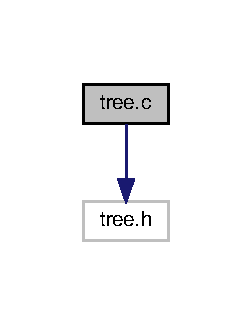
\includegraphics[width=121pt]{tree_8c__incl}
\end{center}
\end{figure}
\subsection*{Estruturas de Dados}
\begin{DoxyCompactItemize}
\item 
struct \hyperlink{structNode}{Node}
\end{DoxyCompactItemize}
\subsection*{Funções}
\begin{DoxyCompactItemize}
\item 
int \hyperlink{tree_8c_a104bddcadd9707197019259239c1a58b}{height} (struct \hyperlink{structNode}{Node} $\ast$N)
\begin{DoxyCompactList}\small\item\em Função que calcula a altura de um nodo. \end{DoxyCompactList}\item 
int \hyperlink{tree_8c_af082905f7eac6d03e92015146bbc1925}{max} (int a, int b)
\begin{DoxyCompactList}\small\item\em Função que devolve o máximo de dois inteiros. \end{DoxyCompactList}\item 
struct \hyperlink{structNode}{Node} $\ast$ \hyperlink{tree_8c_a6ef0036e40936f1377e0774df4a14fa2}{init\+A\+VL} ()
\begin{DoxyCompactList}\small\item\em Inicializa uma A\+VL. \end{DoxyCompactList}\item 
int \hyperlink{tree_8c_afc35ee30a700f9c8eae2a186d262169e}{num\+Node} (A\+VL $\ast$nodo)
\begin{DoxyCompactList}\small\item\em Função que devolve o número de nodos da árvore. \end{DoxyCompactList}\item 
struct \hyperlink{structNode}{Node} $\ast$ \hyperlink{tree_8c_a1c8db440cd3383e117d2b840c00da573}{new\+Node} (char $\ast$key, void $\ast$a)
\begin{DoxyCompactList}\small\item\em Funcao que cria um novo nodo. \end{DoxyCompactList}\item 
struct \hyperlink{structNode}{Node} $\ast$ \hyperlink{tree_8c_a21652fe3310af35bb6d05cc64be6c958}{right\+Rotate} (struct \hyperlink{structNode}{Node} $\ast$y)
\begin{DoxyCompactList}\small\item\em Função que efetua uma rotação da árvore para a direita. \end{DoxyCompactList}\item 
struct \hyperlink{structNode}{Node} $\ast$ \hyperlink{tree_8c_aa14c3e3be03cd95fa83ddf927846ca72}{left\+Rotate} (struct \hyperlink{structNode}{Node} $\ast$x)
\begin{DoxyCompactList}\small\item\em Função que efetua uma rotação da árvore para a esquerda. \end{DoxyCompactList}\item 
int \hyperlink{tree_8c_aa40aa29ef5169ee7f528ea7b7beab43c}{get\+Balance} (struct \hyperlink{structNode}{Node} $\ast$N)
\begin{DoxyCompactList}\small\item\em Função que vê se a arvore é balanceada. \end{DoxyCompactList}\item 
struct \hyperlink{structNode}{Node} $\ast$ \hyperlink{tree_8c_a8792d9847f06c27e4955b63f63239305}{insert} (struct \hyperlink{structNode}{Node} $\ast$node, char $\ast$key, void $\ast$equals)
\begin{DoxyCompactList}\small\item\em Função que insere um elemento na árvore. \end{DoxyCompactList}\item 
\mbox{\Hypertarget{tree_8c_a35c2e83613567d89cecfdd11be4683a5}\label{tree_8c_a35c2e83613567d89cecfdd11be4683a5}} 
A\+VL $\ast$ {\bfseries search\+A\+V\+L\+T\+MP} (A\+VL $\ast$node, char $\ast$key)
\item 
int \hyperlink{tree_8c_a56e7dddb3c67ac22f3373a010c1c9e21}{search\+A\+VL} (A\+VL $\ast$node, char $\ast$key)
\begin{DoxyCompactList}\small\item\em Função que procura um elemento na árvore. \end{DoxyCompactList}\item 
char $\ast$ \hyperlink{tree_8c_af043329377f4d9303267455cd353fd83}{get\+Key} (A\+VL $\ast$a)
\begin{DoxyCompactList}\small\item\em Função que devolve a key de a. \end{DoxyCompactList}\item 
void $\ast$ \hyperlink{tree_8c_a1c2789a702672b4fb99d2c622181f949}{get\+Equals} (A\+VL $\ast$a)
\begin{DoxyCompactList}\small\item\em Função que devolve o equals de a. \end{DoxyCompactList}\item 
A\+VL $\ast$ \hyperlink{tree_8c_a055813fad18fbe1331c4568fbb9b53ca}{get\+Left} (A\+VL $\ast$a)
\begin{DoxyCompactList}\small\item\em Função que devolve a esquerda de a. \end{DoxyCompactList}\item 
A\+VL $\ast$ \hyperlink{tree_8c_aa92a92ff16f40e2381b0452982b620b3}{get\+Right} (A\+VL $\ast$a)
\begin{DoxyCompactList}\small\item\em Função que devolve a direita de a. \end{DoxyCompactList}\end{DoxyCompactItemize}


\subsection{Descrição detalhada}
Ficheiro que contem funções utilizadas na construção da A\+VL utilizada e em todas as funcionalidades por esta suportadas. 



\subsection{Documentação das funções}
\mbox{\Hypertarget{tree_8c_aa40aa29ef5169ee7f528ea7b7beab43c}\label{tree_8c_aa40aa29ef5169ee7f528ea7b7beab43c}} 
\index{tree.\+c@{tree.\+c}!get\+Balance@{get\+Balance}}
\index{get\+Balance@{get\+Balance}!tree.\+c@{tree.\+c}}
\subsubsection{\texorpdfstring{get\+Balance()}{getBalance()}}
{\footnotesize\ttfamily int get\+Balance (\begin{DoxyParamCaption}\item[{struct \hyperlink{structNode}{Node} $\ast$}]{N }\end{DoxyParamCaption})}



Função que vê se a arvore é balanceada. 


\begin{DoxyParams}{Parâmetros}
{\em \mbox{[}\+N\mbox{]}} & Apontador para o nodo \\
\hline
\end{DoxyParams}
\begin{DoxyReturn}{Retorna}
Árvore balanceada 
\end{DoxyReturn}


Definido na linha 134 do ficheiro tree.\+c.


\begin{DoxyCode}
135 \{
136     \textcolor{keywordflow}{if} (N == NULL)
137         \textcolor{keywordflow}{return} 0;
138     \textcolor{keywordflow}{return} \hyperlink{tree_8c_a104bddcadd9707197019259239c1a58b}{height}(N->left) - \hyperlink{tree_8c_a104bddcadd9707197019259239c1a58b}{height}(N->right);
139 \}
\end{DoxyCode}
\mbox{\Hypertarget{tree_8c_a1c2789a702672b4fb99d2c622181f949}\label{tree_8c_a1c2789a702672b4fb99d2c622181f949}} 
\index{tree.\+c@{tree.\+c}!get\+Equals@{get\+Equals}}
\index{get\+Equals@{get\+Equals}!tree.\+c@{tree.\+c}}
\subsubsection{\texorpdfstring{get\+Equals()}{getEquals()}}
{\footnotesize\ttfamily void$\ast$ get\+Equals (\begin{DoxyParamCaption}\item[{A\+VL $\ast$}]{a }\end{DoxyParamCaption})}



Função que devolve o equals de a. 


\begin{DoxyParams}{Parâmetros}
{\em \mbox{[}a\mbox{]}} & a é um apontador do tipo A\+VL \\
\hline
\end{DoxyParams}
\begin{DoxyReturn}{Retorna}
Equals de a 
\end{DoxyReturn}


Definido na linha 236 do ficheiro tree.\+c.


\begin{DoxyCode}
236                        \{
237   \textcolor{keywordflow}{return} (\textcolor{keywordtype}{void}*)a->equals;
238 \}
\end{DoxyCode}
\mbox{\Hypertarget{tree_8c_af043329377f4d9303267455cd353fd83}\label{tree_8c_af043329377f4d9303267455cd353fd83}} 
\index{tree.\+c@{tree.\+c}!get\+Key@{get\+Key}}
\index{get\+Key@{get\+Key}!tree.\+c@{tree.\+c}}
\subsubsection{\texorpdfstring{get\+Key()}{getKey()}}
{\footnotesize\ttfamily char$\ast$ get\+Key (\begin{DoxyParamCaption}\item[{A\+VL $\ast$}]{a }\end{DoxyParamCaption})}



Função que devolve a key de a. 


\begin{DoxyParams}{Parâmetros}
{\em \mbox{[}a\mbox{]}} & a é um apontador do tipo A\+VL \\
\hline
\end{DoxyParams}
\begin{DoxyReturn}{Retorna}
Key de a 
\end{DoxyReturn}


Definido na linha 227 do ficheiro tree.\+c.


\begin{DoxyCode}
227                     \{
228   \textcolor{keywordflow}{return} a->key;
229 \}
\end{DoxyCode}
\mbox{\Hypertarget{tree_8c_a055813fad18fbe1331c4568fbb9b53ca}\label{tree_8c_a055813fad18fbe1331c4568fbb9b53ca}} 
\index{tree.\+c@{tree.\+c}!get\+Left@{get\+Left}}
\index{get\+Left@{get\+Left}!tree.\+c@{tree.\+c}}
\subsubsection{\texorpdfstring{get\+Left()}{getLeft()}}
{\footnotesize\ttfamily A\+VL$\ast$ get\+Left (\begin{DoxyParamCaption}\item[{A\+VL $\ast$}]{a }\end{DoxyParamCaption})}



Função que devolve a esquerda de a. 


\begin{DoxyParams}{Parâmetros}
{\em \mbox{[}a\mbox{]}} & a é um apontador do tipo A\+VL \\
\hline
\end{DoxyParams}
\begin{DoxyReturn}{Retorna}
Esquerda de a 
\end{DoxyReturn}


Definido na linha 245 do ficheiro tree.\+c.


\begin{DoxyCode}
245                      \{
246   \textcolor{keywordflow}{return} a->left;
247 \}
\end{DoxyCode}
\mbox{\Hypertarget{tree_8c_aa92a92ff16f40e2381b0452982b620b3}\label{tree_8c_aa92a92ff16f40e2381b0452982b620b3}} 
\index{tree.\+c@{tree.\+c}!get\+Right@{get\+Right}}
\index{get\+Right@{get\+Right}!tree.\+c@{tree.\+c}}
\subsubsection{\texorpdfstring{get\+Right()}{getRight()}}
{\footnotesize\ttfamily A\+VL$\ast$ get\+Right (\begin{DoxyParamCaption}\item[{A\+VL $\ast$}]{a }\end{DoxyParamCaption})}



Função que devolve a direita de a. 


\begin{DoxyParams}{Parâmetros}
{\em \mbox{[}a\mbox{]}} & a é um apontador do tipo A\+VL \\
\hline
\end{DoxyParams}
\begin{DoxyReturn}{Retorna}
Direita de a 
\end{DoxyReturn}


Definido na linha 254 do ficheiro tree.\+c.


\begin{DoxyCode}
254                       \{
255   \textcolor{keywordflow}{return} a->right;
256 \}
\end{DoxyCode}
\mbox{\Hypertarget{tree_8c_a104bddcadd9707197019259239c1a58b}\label{tree_8c_a104bddcadd9707197019259239c1a58b}} 
\index{tree.\+c@{tree.\+c}!height@{height}}
\index{height@{height}!tree.\+c@{tree.\+c}}
\subsubsection{\texorpdfstring{height()}{height()}}
{\footnotesize\ttfamily int height (\begin{DoxyParamCaption}\item[{struct \hyperlink{structNode}{Node} $\ast$}]{N }\end{DoxyParamCaption})}



Função que calcula a altura de um nodo. 


\begin{DoxyParams}{Parâmetros}
{\em \mbox{[}\+N\mbox{]}} & Apontador para o nodo \\
\hline
\end{DoxyParams}
\begin{DoxyReturn}{Retorna}
Altura de um nodo 
\end{DoxyReturn}


Definido na linha 22 do ficheiro tree.\+c.


\begin{DoxyCode}
23 \{
24     \textcolor{keywordflow}{if} (N == NULL)
25         \textcolor{keywordflow}{return} 0;
26     \textcolor{keywordflow}{return} N->height;
27 \}
\end{DoxyCode}
\mbox{\Hypertarget{tree_8c_a6ef0036e40936f1377e0774df4a14fa2}\label{tree_8c_a6ef0036e40936f1377e0774df4a14fa2}} 
\index{tree.\+c@{tree.\+c}!init\+A\+VL@{init\+A\+VL}}
\index{init\+A\+VL@{init\+A\+VL}!tree.\+c@{tree.\+c}}
\subsubsection{\texorpdfstring{init\+A\+V\+L()}{initAVL()}}
{\footnotesize\ttfamily struct \hyperlink{structNode}{Node}$\ast$ init\+A\+VL (\begin{DoxyParamCaption}{ }\end{DoxyParamCaption})}



Inicializa uma A\+VL. 

\begin{DoxyReturn}{Retorna}
Retorna a A\+VL inicializada 
\end{DoxyReturn}


Definido na linha 46 do ficheiro tree.\+c.


\begin{DoxyCode}
46                        \{
47   AVL* a = malloc(\textcolor{keyword}{sizeof}(AVL));
48   a->key = NULL;
49   a->left = NULL;
50   a->height = 0;
51   a->right = NULL;
52   a->equals = NULL;
53   \textcolor{keywordflow}{return} a;
54 \}
\end{DoxyCode}
\mbox{\Hypertarget{tree_8c_a8792d9847f06c27e4955b63f63239305}\label{tree_8c_a8792d9847f06c27e4955b63f63239305}} 
\index{tree.\+c@{tree.\+c}!insert@{insert}}
\index{insert@{insert}!tree.\+c@{tree.\+c}}
\subsubsection{\texorpdfstring{insert()}{insert()}}
{\footnotesize\ttfamily struct \hyperlink{structNode}{Node}$\ast$ insert (\begin{DoxyParamCaption}\item[{struct \hyperlink{structNode}{Node} $\ast$}]{node,  }\item[{char $\ast$}]{key,  }\item[{void $\ast$}]{equals }\end{DoxyParamCaption})}



Função que insere um elemento na árvore. 


\begin{DoxyParams}{Parâmetros}
{\em \mbox{[}node\mbox{]}} & \hyperlink{structNode}{Node} é um apontador para a struct \\
\hline
{\em \mbox{[}key\mbox{]}} & Key é um apontador de um char \\
\hline
{\em \mbox{[}equals\mbox{]}} & Equals é um apontador de um void \\
\hline
\end{DoxyParams}
\begin{DoxyReturn}{Retorna}
Apontador para a estrutura após ter sido inserido o valor 
\end{DoxyReturn}


Definido na linha 149 do ficheiro tree.\+c.


\begin{DoxyCode}
150 \{
151 
152     \textcolor{keywordflow}{if} (node == NULL)
153         \textcolor{keywordflow}{return}(\hyperlink{tree_8c_a1c8db440cd3383e117d2b840c00da573}{newNode}(key,equals));
154 
155     \textcolor{keywordflow}{if} ((strcmp(key, node->key)) < 0)
156         node->left  = \hyperlink{tree_8c_a8792d9847f06c27e4955b63f63239305}{insert}(node->left, key,equals);
157     \textcolor{keywordflow}{else} \textcolor{keywordflow}{if} (strcmp(key, node->key) > 0)
158         node->right = \hyperlink{tree_8c_a8792d9847f06c27e4955b63f63239305}{insert}(node->right, key,equals);
159 
160     node->height = 1 + \hyperlink{tree_8c_af082905f7eac6d03e92015146bbc1925}{max}(\hyperlink{tree_8c_a104bddcadd9707197019259239c1a58b}{height}(node->left),
161                            \hyperlink{tree_8c_a104bddcadd9707197019259239c1a58b}{height}(node->right));
162 
163 
164 
165     \textcolor{keywordtype}{int} balance = \hyperlink{tree_8c_aa40aa29ef5169ee7f528ea7b7beab43c}{getBalance}(node);
166 
167     \textcolor{keywordflow}{if} (balance > 1 && strcmp(key, node->left->key) < 0)
168         \textcolor{keywordflow}{return} \hyperlink{tree_8c_a21652fe3310af35bb6d05cc64be6c958}{rightRotate}(node);
169 
170     \textcolor{keywordflow}{if} (balance < -1 && strcmp(key, node->right->key) >= 0)
171         \textcolor{keywordflow}{return} \hyperlink{tree_8c_aa14c3e3be03cd95fa83ddf927846ca72}{leftRotate}(node);
172 
173     \textcolor{keywordflow}{if} (balance > 1 && strcmp(key, node->left->key) >= 0)
174     \{
175         node->left =  \hyperlink{tree_8c_aa14c3e3be03cd95fa83ddf927846ca72}{leftRotate}(node->left);
176         \textcolor{keywordflow}{return} \hyperlink{tree_8c_a21652fe3310af35bb6d05cc64be6c958}{rightRotate}(node);
177     \}
178 
179     \textcolor{keywordflow}{if} (balance < -1 && strcmp(key, node->right->key) < 0)
180     \{
181         node->right = \hyperlink{tree_8c_a21652fe3310af35bb6d05cc64be6c958}{rightRotate}(node->right);
182         \textcolor{keywordflow}{return} \hyperlink{tree_8c_aa14c3e3be03cd95fa83ddf927846ca72}{leftRotate}(node);
183     \}
184 
185     \textcolor{keywordflow}{return} node;
186 \}
\end{DoxyCode}
\mbox{\Hypertarget{tree_8c_aa14c3e3be03cd95fa83ddf927846ca72}\label{tree_8c_aa14c3e3be03cd95fa83ddf927846ca72}} 
\index{tree.\+c@{tree.\+c}!left\+Rotate@{left\+Rotate}}
\index{left\+Rotate@{left\+Rotate}!tree.\+c@{tree.\+c}}
\subsubsection{\texorpdfstring{left\+Rotate()}{leftRotate()}}
{\footnotesize\ttfamily struct \hyperlink{structNode}{Node}$\ast$ left\+Rotate (\begin{DoxyParamCaption}\item[{struct \hyperlink{structNode}{Node} $\ast$}]{x }\end{DoxyParamCaption})}



Função que efetua uma rotação da árvore para a esquerda. 


\begin{DoxyParams}{Parâmetros}
{\em \mbox{[}x\mbox{]}} & Apontador para o nodo \\
\hline
\end{DoxyParams}
\begin{DoxyReturn}{Retorna}
Árvore após ser rodada para a esquerda 
\end{DoxyReturn}


Definido na linha 114 do ficheiro tree.\+c.


\begin{DoxyCode}
115 \{
116     \textcolor{keyword}{struct }\hyperlink{structNode}{Node} *y = x->right;
117     \textcolor{keyword}{struct }\hyperlink{structNode}{Node} *T2 = y->left;
118 
119     y->left = x;
120     x->right = T2;
121 
122     x->height = \hyperlink{tree_8c_af082905f7eac6d03e92015146bbc1925}{max}(\hyperlink{tree_8c_a104bddcadd9707197019259239c1a58b}{height}(x->left), \hyperlink{tree_8c_a104bddcadd9707197019259239c1a58b}{height}(x->right))+1;
123     y->height = \hyperlink{tree_8c_af082905f7eac6d03e92015146bbc1925}{max}(\hyperlink{tree_8c_a104bddcadd9707197019259239c1a58b}{height}(y->left), \hyperlink{tree_8c_a104bddcadd9707197019259239c1a58b}{height}(y->right))+1;
124 
125     \textcolor{keywordflow}{return} y;
126 \}
\end{DoxyCode}
\mbox{\Hypertarget{tree_8c_af082905f7eac6d03e92015146bbc1925}\label{tree_8c_af082905f7eac6d03e92015146bbc1925}} 
\index{tree.\+c@{tree.\+c}!max@{max}}
\index{max@{max}!tree.\+c@{tree.\+c}}
\subsubsection{\texorpdfstring{max()}{max()}}
{\footnotesize\ttfamily int max (\begin{DoxyParamCaption}\item[{int}]{a,  }\item[{int}]{b }\end{DoxyParamCaption})}



Função que devolve o máximo de dois inteiros. 


\begin{DoxyParams}{Parâmetros}
{\em \mbox{[}a\mbox{]}} & Um dos inteiros para comparação \\
\hline
{\em \mbox{[}b\mbox{]}} & Um dos inteiros para comparação \\
\hline
\end{DoxyParams}
\begin{DoxyReturn}{Retorna}
Máximo entre dois inteiros 
\end{DoxyReturn}


Definido na linha 36 do ficheiro tree.\+c.


\begin{DoxyCode}
37 \{
38     \textcolor{keywordflow}{return} (a > b)? a : b;
39 \}
\end{DoxyCode}
\mbox{\Hypertarget{tree_8c_a1c8db440cd3383e117d2b840c00da573}\label{tree_8c_a1c8db440cd3383e117d2b840c00da573}} 
\index{tree.\+c@{tree.\+c}!new\+Node@{new\+Node}}
\index{new\+Node@{new\+Node}!tree.\+c@{tree.\+c}}
\subsubsection{\texorpdfstring{new\+Node()}{newNode()}}
{\footnotesize\ttfamily struct \hyperlink{structNode}{Node}$\ast$ new\+Node (\begin{DoxyParamCaption}\item[{char $\ast$}]{key,  }\item[{void $\ast$}]{a }\end{DoxyParamCaption})}



Funcao que cria um novo nodo. 


\begin{DoxyParams}{Parâmetros}
{\em \mbox{[}key\mbox{]}} & Char$\ast$ utilizado para a key da arvore \\
\hline
{\em \mbox{[}equals\mbox{]}} & Parametro void que será inserido no equals da A\+VL \\
\hline
\end{DoxyParams}
\begin{DoxyReturn}{Retorna}
Retorna o novo nodo 
\end{DoxyReturn}


Definido na linha 76 do ficheiro tree.\+c.


\begin{DoxyCode}
77 \{
78     \textcolor{keyword}{struct }\hyperlink{structNode}{Node}* node = (\textcolor{keyword}{struct }\hyperlink{structNode}{Node}*)
79                         malloc(\textcolor{keyword}{sizeof}(\textcolor{keyword}{struct} \hyperlink{structNode}{Node}));
80     node->key = key;
81     node->left = NULL;
82     node->right = NULL;
83     node->height = 1;
84     node->equals = a;
85 
86     \textcolor{keywordflow}{return}(node);
87 \}
\end{DoxyCode}
\mbox{\Hypertarget{tree_8c_afc35ee30a700f9c8eae2a186d262169e}\label{tree_8c_afc35ee30a700f9c8eae2a186d262169e}} 
\index{tree.\+c@{tree.\+c}!num\+Node@{num\+Node}}
\index{num\+Node@{num\+Node}!tree.\+c@{tree.\+c}}
\subsubsection{\texorpdfstring{num\+Node()}{numNode()}}
{\footnotesize\ttfamily int num\+Node (\begin{DoxyParamCaption}\item[{A\+VL $\ast$}]{nodo }\end{DoxyParamCaption})}



Função que devolve o número de nodos da árvore. 


\begin{DoxyParams}{Parâmetros}
{\em \mbox{[}nodo\mbox{]}} & Nodo é um apontador do tipo A\+VL \\
\hline
\end{DoxyParams}
\begin{DoxyReturn}{Retorna}
Numero de nodos da árvore 
\end{DoxyReturn}


Definido na linha 62 do ficheiro tree.\+c.


\begin{DoxyCode}
62                       \{
63   \textcolor{keywordflow}{if} (nodo)\{
64     \textcolor{keywordflow}{return} 1 + \hyperlink{tree_8c_afc35ee30a700f9c8eae2a186d262169e}{numNode}(nodo->left) + \hyperlink{tree_8c_afc35ee30a700f9c8eae2a186d262169e}{numNode}(nodo->right);
65   \}
66   \textcolor{keywordflow}{else} \textcolor{keywordflow}{return} 0;
67 \}
\end{DoxyCode}
\mbox{\Hypertarget{tree_8c_a21652fe3310af35bb6d05cc64be6c958}\label{tree_8c_a21652fe3310af35bb6d05cc64be6c958}} 
\index{tree.\+c@{tree.\+c}!right\+Rotate@{right\+Rotate}}
\index{right\+Rotate@{right\+Rotate}!tree.\+c@{tree.\+c}}
\subsubsection{\texorpdfstring{right\+Rotate()}{rightRotate()}}
{\footnotesize\ttfamily struct \hyperlink{structNode}{Node}$\ast$ right\+Rotate (\begin{DoxyParamCaption}\item[{struct \hyperlink{structNode}{Node} $\ast$}]{y }\end{DoxyParamCaption})}



Função que efetua uma rotação da árvore para a direita. 


\begin{DoxyParams}{Parâmetros}
{\em \mbox{[}y\mbox{]}} & Apontador para o nodo \\
\hline
\end{DoxyParams}
\begin{DoxyReturn}{Retorna}
Árvore após ser rodada para a direita 
\end{DoxyReturn}


Definido na linha 94 do ficheiro tree.\+c.


\begin{DoxyCode}
95 \{
96     \textcolor{keyword}{struct }\hyperlink{structNode}{Node} *x = y->left;
97     \textcolor{keyword}{struct }\hyperlink{structNode}{Node} *T2 = x->right;
98 
99     x->right = y;
100     y->left = T2;
101 
102     y->height = \hyperlink{tree_8c_af082905f7eac6d03e92015146bbc1925}{max}(\hyperlink{tree_8c_a104bddcadd9707197019259239c1a58b}{height}(y->left), \hyperlink{tree_8c_a104bddcadd9707197019259239c1a58b}{height}(y->right))+1;
103     x->height = \hyperlink{tree_8c_af082905f7eac6d03e92015146bbc1925}{max}(\hyperlink{tree_8c_a104bddcadd9707197019259239c1a58b}{height}(x->left), \hyperlink{tree_8c_a104bddcadd9707197019259239c1a58b}{height}(x->right))+1;
104 
105     \textcolor{keywordflow}{return} x;
106 \}
\end{DoxyCode}
\mbox{\Hypertarget{tree_8c_a56e7dddb3c67ac22f3373a010c1c9e21}\label{tree_8c_a56e7dddb3c67ac22f3373a010c1c9e21}} 
\index{tree.\+c@{tree.\+c}!search\+A\+VL@{search\+A\+VL}}
\index{search\+A\+VL@{search\+A\+VL}!tree.\+c@{tree.\+c}}
\subsubsection{\texorpdfstring{search\+A\+V\+L()}{searchAVL()}}
{\footnotesize\ttfamily int search\+A\+VL (\begin{DoxyParamCaption}\item[{A\+VL $\ast$}]{node,  }\item[{char $\ast$}]{key }\end{DoxyParamCaption})}



Função que procura um elemento na árvore. 

\} 
\begin{DoxyParams}{Parâmetros}
{\em \mbox{[}node\mbox{]}} & Nodo é um apontador do tipo A\+VL \\
\hline
{\em \mbox{[}key\mbox{]}} & Key é um apontador de um char \\
\hline
\end{DoxyParams}
\begin{DoxyReturn}{Retorna}
Resultado da procura, retornando 0 caso essa procura falhe 
\end{DoxyReturn}


Definido na linha 208 do ficheiro tree.\+c.


\begin{DoxyCode}
208                                     \{
209 
210     \textcolor{keywordflow}{if}(node == NULL)
211         \textcolor{keywordflow}{return} 0;
212     \textcolor{keywordflow}{if}(strcmp(node->key,key) == 0)
213         \textcolor{keywordflow}{return} 1;
214     \textcolor{keywordflow}{if}(strcmp(node->key,key) < 0)
215         \textcolor{keywordflow}{return} \hyperlink{tree_8c_a56e7dddb3c67ac22f3373a010c1c9e21}{searchAVL}(node->right,key);
216     \textcolor{keywordflow}{else}
217         \textcolor{keywordflow}{return} \hyperlink{tree_8c_a56e7dddb3c67ac22f3373a010c1c9e21}{searchAVL}(node->left,key);
218 
219 \}
\end{DoxyCode}

\hypertarget{vendas_8c}{}\section{Referência ao ficheiro vendas.\+c}
\label{vendas_8c}\index{vendas.\+c@{vendas.\+c}}


Ficheiro que contem funções utilizadas para as vendas.  


{\ttfamily \#include \char`\"{}vendas.\+h\char`\"{}}\newline
Diagrama de dependências de inclusão para vendas.\+c\+:
\nopagebreak
\begin{figure}[H]
\begin{center}
\leavevmode
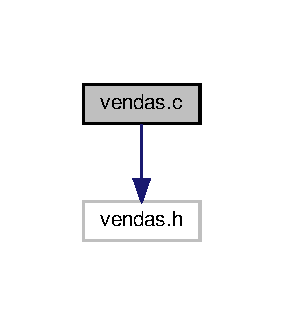
\includegraphics[width=136pt]{vendas_8c__incl}
\end{center}
\end{figure}
\subsection*{Estruturas de Dados}
\begin{DoxyCompactItemize}
\item 
struct \hyperlink{structvenda}{venda}
\item 
struct \hyperlink{structvt}{vt}
\end{DoxyCompactItemize}
\subsection*{Funções}
\begin{DoxyCompactItemize}
\item 
VT $\ast$ \hyperlink{vendas_8c_a2e874e42b7b9192295e9d78409212f12}{init\+Vendas} ()
\begin{DoxyCompactList}\small\item\em Inicialização dos dados das vendas. \end{DoxyCompactList}\item 
void \hyperlink{vendas_8c_a3a676f1271229cc890ba52aaba7d56d3}{free\+Vendas} (VT $\ast$v)
\begin{DoxyCompactList}\small\item\em Função que desaloca a memória ocupada pelas Vendas. \end{DoxyCompactList}\item 
void \hyperlink{vendas_8c_a25285041e9e1c908308ef567fc4b4d33}{realloc\+Vendas} (VT $\ast$v)
\begin{DoxyCompactList}\small\item\em Função que realoca a memoria ocupada pelas Vendas. \end{DoxyCompactList}\item 
int \hyperlink{vendas_8c_af6a785d1d84f6615746c6fcc1143145a}{binary\+Search} (char $\ast$$\ast$total, int i, int t, char $\ast$str)
\begin{DoxyCompactList}\small\item\em Função que efetua a procura binária. \end{DoxyCompactList}\item 
int \hyperlink{vendas_8c_a1c768f74950721cd51fbc852da5cd724}{product} (char $\ast$prod, Dados $\ast$produtos)
\begin{DoxyCompactList}\small\item\em Valida a componente produto. \end{DoxyCompactList}\item 
int \hyperlink{vendas_8c_a80f8707201f9b5119865530aeb3515fe}{price} (double preco)
\begin{DoxyCompactList}\small\item\em Valida a componente preço. \end{DoxyCompactList}\item 
int \hyperlink{vendas_8c_a22147cd1e2e6a4da0d9a7b78f1936e30}{quantity} (int quant)
\begin{DoxyCompactList}\small\item\em Valida a componente quantidade. \end{DoxyCompactList}\item 
int \hyperlink{vendas_8c_a4d8bdada7a6ca4234e17a0f4c958ffdc}{promotion} (char prom)
\begin{DoxyCompactList}\small\item\em Valida a componente promoção. \end{DoxyCompactList}\item 
int \hyperlink{vendas_8c_ab5f658c9a3766364fea66a37c7d355d6}{client} (char $\ast$cli, Dados $\ast$clientes)
\begin{DoxyCompactList}\small\item\em Valida a componente cliente. \end{DoxyCompactList}\item 
int \hyperlink{vendas_8c_a0b4bbe164a873e171e9758176de52d7f}{month} (int mes)
\begin{DoxyCompactList}\small\item\em Valida a componente mês. \end{DoxyCompactList}\item 
int \hyperlink{vendas_8c_a8f8279380cac3393546f9d2d54b55493}{market} (int super)
\begin{DoxyCompactList}\small\item\em Valida a componente filial. \end{DoxyCompactList}\item 
int \hyperlink{vendas_8c_a27df57465f246def8fbfe1b822b996fb}{valid\+\_\+\+Venda} (char $\ast$prod, double preco, int quant, char prom, char $\ast$cli, int mes, int super, Dados $\ast$produtos, Dados $\ast$clientes)
\begin{DoxyCompactList}\small\item\em Valida a componente venda. \end{DoxyCompactList}\item 
char $\ast$ \hyperlink{vendas_8c_a44aa4bbfb64f14bb33fefaeb575c00e1}{get\+Produto} (Venda $\ast$v)
\begin{DoxyCompactList}\small\item\em Acesso à componente produto. \end{DoxyCompactList}\item 
double \hyperlink{vendas_8c_a9cde304721e7cf45c51ec95bcf625de4}{get\+Preco} (Venda $\ast$v)
\begin{DoxyCompactList}\small\item\em Acesso à componente preço. \end{DoxyCompactList}\item 
int \hyperlink{vendas_8c_ae3196cffdcf5289440c1ee56ed5ee0d7}{get\+Quantidade} (Venda $\ast$v)
\begin{DoxyCompactList}\small\item\em Acesso à componente quantidade. \end{DoxyCompactList}\item 
int \hyperlink{vendas_8c_ac48ab849f5af46f09394a208f41029e6}{get\+Promocao} (Venda $\ast$v)
\begin{DoxyCompactList}\small\item\em Acesso à componente promoção. \end{DoxyCompactList}\item 
char $\ast$ \hyperlink{vendas_8c_a6a66082eb395bd8876be3504c51aa264}{get\+Cliente} (Venda $\ast$v)
\begin{DoxyCompactList}\small\item\em Acesso à componente cliente. \end{DoxyCompactList}\item 
int \hyperlink{vendas_8c_a1178cf1dea33bcb6c9612d46f7534f33}{get\+Data} (Venda $\ast$v)
\begin{DoxyCompactList}\small\item\em Acesso à componente data. \end{DoxyCompactList}\item 
int \hyperlink{vendas_8c_a7381c97aa7302d679514ddbeabb1753f}{get\+Filial} (Venda $\ast$v)
\begin{DoxyCompactList}\small\item\em Acesso à componente filial. \end{DoxyCompactList}\item 
void \hyperlink{vendas_8c_a46d5e820149ab77e7379f18e9dd5658f}{read\+\_\+\+Vendas} (VT $\ast$vendas, Dados $\ast$produtos, Dados $\ast$clientes, char $\ast$file\+Path)
\begin{DoxyCompactList}\small\item\em Função que lê um ficheiro .txt com a informacao relativa às vendas. \end{DoxyCompactList}\item 
int \hyperlink{vendas_8c_aba67c7ea52fab81d42a891082b59ef72}{get\+OcupadosV} (VT $\ast$vendas)
\begin{DoxyCompactList}\small\item\em Função que devolve o espaço ocupado pelas vendas na string. \end{DoxyCompactList}\item 
int \hyperlink{vendas_8c_a370fea8a0d2e5993f27e8f79ca016f07}{get\+LidasV} (VT $\ast$vendas)
\begin{DoxyCompactList}\small\item\em Função que devolve as vendas lidas. \end{DoxyCompactList}\item 
Venda $\ast$ \hyperlink{vendas_8c_ab7121d1c08c763f3f6f3ab5902682ecd}{get\+Venda} (VT $\ast$vendas, int i)
\begin{DoxyCompactList}\small\item\em Função que devolve um array com as vendas. \end{DoxyCompactList}\end{DoxyCompactItemize}


\subsection{Descrição detalhada}
Ficheiro que contem funções utilizadas para as vendas. 



\subsection{Documentação das funções}
\mbox{\Hypertarget{vendas_8c_af6a785d1d84f6615746c6fcc1143145a}\label{vendas_8c_af6a785d1d84f6615746c6fcc1143145a}} 
\index{vendas.\+c@{vendas.\+c}!binary\+Search@{binary\+Search}}
\index{binary\+Search@{binary\+Search}!vendas.\+c@{vendas.\+c}}
\subsubsection{\texorpdfstring{binary\+Search()}{binarySearch()}}
{\footnotesize\ttfamily int binary\+Search (\begin{DoxyParamCaption}\item[{char $\ast$$\ast$}]{total,  }\item[{int}]{i,  }\item[{int}]{t,  }\item[{char $\ast$}]{str }\end{DoxyParamCaption})}



Função que efetua a procura binária. 


\begin{DoxyParams}{Parâmetros}
{\em \mbox{[}total\mbox{]}} & char$\ast$$\ast$ onde queremos fazer a procura \\
\hline
{\em \mbox{[}i\mbox{]}} & Indice i \\
\hline
{\em \mbox{[}t\mbox{]}} & Indice t \\
\hline
{\em \mbox{[}str\mbox{]}} & char$\ast$ que queremos encontrar \\
\hline
\end{DoxyParams}
\begin{DoxyReturn}{Retorna}
Retorna -\/1 caso a procura falhe 
\end{DoxyReturn}


Definido na linha 94 do ficheiro vendas.\+c.


\begin{DoxyCode}
95 \{
96     \textcolor{keywordflow}{while} (i <= t) \{
97         \textcolor{keywordtype}{int} m = i + (t - i) / 2;
98 
99         \textcolor{keywordflow}{if} (strcmp(total[m],str) == 0)
100             \textcolor{keywordflow}{return} m;
101         \textcolor{keywordflow}{if} (strcmp(total[m],str) < 0)
102             i = m + 1;
103         \textcolor{keywordflow}{else}
104             t = m - 1;
105     \}
106     \textcolor{keywordflow}{return} -1;
107 \}
\end{DoxyCode}
\mbox{\Hypertarget{vendas_8c_ab5f658c9a3766364fea66a37c7d355d6}\label{vendas_8c_ab5f658c9a3766364fea66a37c7d355d6}} 
\index{vendas.\+c@{vendas.\+c}!client@{client}}
\index{client@{client}!vendas.\+c@{vendas.\+c}}
\subsubsection{\texorpdfstring{client()}{client()}}
{\footnotesize\ttfamily int client (\begin{DoxyParamCaption}\item[{char $\ast$}]{cli,  }\item[{Dados $\ast$}]{clientes }\end{DoxyParamCaption})}



Valida a componente cliente. 


\begin{DoxyParams}{Parâmetros}
{\em \mbox{[}prod\mbox{]}} & Cliente \\
\hline
\end{DoxyParams}
\begin{DoxyReturn}{Retorna}
Um r que nos diz se um cliente é validado (r=1) ou não (r=0) 
\end{DoxyReturn}


Definido na linha 165 do ficheiro vendas.\+c.


\begin{DoxyCode}
165                                        \{
166   \textcolor{keywordtype}{int} r = 0;
167   \textcolor{keywordflow}{if} ((\hyperlink{vendas_8c_af6a785d1d84f6615746c6fcc1143145a}{binarySearch}(clientes->str,0,(clientes->ocupados)-1,cli)) != -1)\{
168     r = 1;
169   \}
170   \textcolor{keywordflow}{return} r;
171 \}
\end{DoxyCode}
\mbox{\Hypertarget{vendas_8c_a3a676f1271229cc890ba52aaba7d56d3}\label{vendas_8c_a3a676f1271229cc890ba52aaba7d56d3}} 
\index{vendas.\+c@{vendas.\+c}!free\+Vendas@{free\+Vendas}}
\index{free\+Vendas@{free\+Vendas}!vendas.\+c@{vendas.\+c}}
\subsubsection{\texorpdfstring{free\+Vendas()}{freeVendas()}}
{\footnotesize\ttfamily void free\+Vendas (\begin{DoxyParamCaption}\item[{VT $\ast$}]{v }\end{DoxyParamCaption})}



Função que desaloca a memória ocupada pelas Vendas. 


\begin{DoxyParams}{Parâmetros}
{\em \mbox{[}d\mbox{]}} & uma venda \\
\hline
\end{DoxyParams}


Definido na linha 44 do ficheiro vendas.\+c.


\begin{DoxyCode}
44                       \{
45   \textcolor{keywordtype}{int} i = 0;
46   \textcolor{keywordflow}{for}(i = 0; i < v->ocupados; i++)\{
47     free(v->str[i].produto);
48     v->str[i].produto = NULL;
49     free(v->str[i].cliente);
50     v->str[i].cliente = NULL;
51   \}
52   free(v->str);
53   v->str = NULL;
54   free(v);
55   v = NULL;
56 \}
\end{DoxyCode}
\mbox{\Hypertarget{vendas_8c_a6a66082eb395bd8876be3504c51aa264}\label{vendas_8c_a6a66082eb395bd8876be3504c51aa264}} 
\index{vendas.\+c@{vendas.\+c}!get\+Cliente@{get\+Cliente}}
\index{get\+Cliente@{get\+Cliente}!vendas.\+c@{vendas.\+c}}
\subsubsection{\texorpdfstring{get\+Cliente()}{getCliente()}}
{\footnotesize\ttfamily char$\ast$ get\+Cliente (\begin{DoxyParamCaption}\item[{Venda $\ast$}]{v }\end{DoxyParamCaption})}



Acesso à componente cliente. 


\begin{DoxyParams}{Parâmetros}
{\em \mbox{[}v\mbox{]}} & Uma venda \\
\hline
\end{DoxyParams}
\begin{DoxyReturn}{Retorna}
Um cliente 
\end{DoxyReturn}


Definido na linha 283 do ficheiro vendas.\+c.


\begin{DoxyCode}
283                           \{
284   \textcolor{keywordflow}{return} strdup(v->cliente);
285 \}
\end{DoxyCode}
\mbox{\Hypertarget{vendas_8c_a1178cf1dea33bcb6c9612d46f7534f33}\label{vendas_8c_a1178cf1dea33bcb6c9612d46f7534f33}} 
\index{vendas.\+c@{vendas.\+c}!get\+Data@{get\+Data}}
\index{get\+Data@{get\+Data}!vendas.\+c@{vendas.\+c}}
\subsubsection{\texorpdfstring{get\+Data()}{getData()}}
{\footnotesize\ttfamily int get\+Data (\begin{DoxyParamCaption}\item[{Venda $\ast$}]{v }\end{DoxyParamCaption})}



Acesso à componente data. 


\begin{DoxyParams}{Parâmetros}
{\em \mbox{[}v\mbox{]}} & Uma venda \\
\hline
\end{DoxyParams}
\begin{DoxyReturn}{Retorna}
Uma data 
\end{DoxyReturn}


Definido na linha 293 do ficheiro vendas.\+c.


\begin{DoxyCode}
293                       \{
294   \textcolor{keywordflow}{return} v->data;
295 \}
\end{DoxyCode}
\mbox{\Hypertarget{vendas_8c_a7381c97aa7302d679514ddbeabb1753f}\label{vendas_8c_a7381c97aa7302d679514ddbeabb1753f}} 
\index{vendas.\+c@{vendas.\+c}!get\+Filial@{get\+Filial}}
\index{get\+Filial@{get\+Filial}!vendas.\+c@{vendas.\+c}}
\subsubsection{\texorpdfstring{get\+Filial()}{getFilial()}}
{\footnotesize\ttfamily int get\+Filial (\begin{DoxyParamCaption}\item[{Venda $\ast$}]{v }\end{DoxyParamCaption})}



Acesso à componente filial. 


\begin{DoxyParams}{Parâmetros}
{\em \mbox{[}v\mbox{]}} & Uma venda \\
\hline
\end{DoxyParams}
\begin{DoxyReturn}{Retorna}
Uma filial 
\end{DoxyReturn}


Definido na linha 303 do ficheiro vendas.\+c.


\begin{DoxyCode}
303                         \{
304   \textcolor{keywordflow}{return} v->filial;
305 \}
\end{DoxyCode}
\mbox{\Hypertarget{vendas_8c_a370fea8a0d2e5993f27e8f79ca016f07}\label{vendas_8c_a370fea8a0d2e5993f27e8f79ca016f07}} 
\index{vendas.\+c@{vendas.\+c}!get\+LidasV@{get\+LidasV}}
\index{get\+LidasV@{get\+LidasV}!vendas.\+c@{vendas.\+c}}
\subsubsection{\texorpdfstring{get\+Lidas\+V()}{getLidasV()}}
{\footnotesize\ttfamily int get\+LidasV (\begin{DoxyParamCaption}\item[{VT $\ast$}]{vendas }\end{DoxyParamCaption})}



Função que devolve as vendas lidas. 


\begin{DoxyParams}{Parâmetros}
{\em \mbox{[}produtos\mbox{]}} & Vendas \\
\hline
\end{DoxyParams}
\begin{DoxyReturn}{Retorna}
Vendas lidas 
\end{DoxyReturn}


Definido na linha 366 do ficheiro vendas.\+c.


\begin{DoxyCode}
366                           \{
367   \textcolor{keywordflow}{return} vendas->lidas;
368 \}
\end{DoxyCode}
\mbox{\Hypertarget{vendas_8c_aba67c7ea52fab81d42a891082b59ef72}\label{vendas_8c_aba67c7ea52fab81d42a891082b59ef72}} 
\index{vendas.\+c@{vendas.\+c}!get\+OcupadosV@{get\+OcupadosV}}
\index{get\+OcupadosV@{get\+OcupadosV}!vendas.\+c@{vendas.\+c}}
\subsubsection{\texorpdfstring{get\+Ocupados\+V()}{getOcupadosV()}}
{\footnotesize\ttfamily int get\+OcupadosV (\begin{DoxyParamCaption}\item[{VT $\ast$}]{vendas }\end{DoxyParamCaption})}



Função que devolve o espaço ocupado pelas vendas na string. 


\begin{DoxyParams}{Parâmetros}
{\em \mbox{[}produtos\mbox{]}} & Vendas \\
\hline
\end{DoxyParams}
\begin{DoxyReturn}{Retorna}
Espaço ocupado pelas vendas na string 
\end{DoxyReturn}


Definido na linha 356 do ficheiro vendas.\+c.


\begin{DoxyCode}
356                              \{
357   \textcolor{keywordflow}{return} vendas->ocupados;
358 \}
\end{DoxyCode}
\mbox{\Hypertarget{vendas_8c_a9cde304721e7cf45c51ec95bcf625de4}\label{vendas_8c_a9cde304721e7cf45c51ec95bcf625de4}} 
\index{vendas.\+c@{vendas.\+c}!get\+Preco@{get\+Preco}}
\index{get\+Preco@{get\+Preco}!vendas.\+c@{vendas.\+c}}
\subsubsection{\texorpdfstring{get\+Preco()}{getPreco()}}
{\footnotesize\ttfamily double get\+Preco (\begin{DoxyParamCaption}\item[{Venda $\ast$}]{v }\end{DoxyParamCaption})}



Acesso à componente preço. 


\begin{DoxyParams}{Parâmetros}
{\em \mbox{[}v\mbox{]}} & Uma venda \\
\hline
\end{DoxyParams}
\begin{DoxyReturn}{Retorna}
Um preço 
\end{DoxyReturn}


Definido na linha 248 do ficheiro vendas.\+c.


\begin{DoxyCode}
248                          \{
249   \textcolor{keywordflow}{return} v->preco;
250 \}
\end{DoxyCode}
\mbox{\Hypertarget{vendas_8c_a44aa4bbfb64f14bb33fefaeb575c00e1}\label{vendas_8c_a44aa4bbfb64f14bb33fefaeb575c00e1}} 
\index{vendas.\+c@{vendas.\+c}!get\+Produto@{get\+Produto}}
\index{get\+Produto@{get\+Produto}!vendas.\+c@{vendas.\+c}}
\subsubsection{\texorpdfstring{get\+Produto()}{getProduto()}}
{\footnotesize\ttfamily char$\ast$ get\+Produto (\begin{DoxyParamCaption}\item[{Venda $\ast$}]{v }\end{DoxyParamCaption})}



Acesso à componente produto. 


\begin{DoxyParams}{Parâmetros}
{\em \mbox{[}v\mbox{]}} & Uma venda \\
\hline
\end{DoxyParams}
\begin{DoxyReturn}{Retorna}
Um produto 
\end{DoxyReturn}


Definido na linha 238 do ficheiro vendas.\+c.


\begin{DoxyCode}
238                          \{
239   \textcolor{keywordflow}{return} strdup(v->produto);
240 \}
\end{DoxyCode}
\mbox{\Hypertarget{vendas_8c_ac48ab849f5af46f09394a208f41029e6}\label{vendas_8c_ac48ab849f5af46f09394a208f41029e6}} 
\index{vendas.\+c@{vendas.\+c}!get\+Promocao@{get\+Promocao}}
\index{get\+Promocao@{get\+Promocao}!vendas.\+c@{vendas.\+c}}
\subsubsection{\texorpdfstring{get\+Promocao()}{getPromocao()}}
{\footnotesize\ttfamily int get\+Promocao (\begin{DoxyParamCaption}\item[{Venda $\ast$}]{v }\end{DoxyParamCaption})}



Acesso à componente promoção. 


\begin{DoxyParams}{Parâmetros}
{\em \mbox{[}v\mbox{]}} & Uma venda \\
\hline
\end{DoxyParams}
\begin{DoxyReturn}{Retorna}
Um r que nos diz se uma promoção é do tipo P (r=1) ou do tipo N (r=0) 
\end{DoxyReturn}


Definido na linha 268 do ficheiro vendas.\+c.


\begin{DoxyCode}
268                          \{
269   \textcolor{keywordtype}{int} r = 0;
270   \textcolor{keywordflow}{if} (v->promocao == \textcolor{charliteral}{'N'})
271     r = 0;
272   \textcolor{keywordflow}{else} \textcolor{keywordflow}{if}(v->promocao == \textcolor{charliteral}{'P'})
273     r = 1;
274   \textcolor{keywordflow}{return} r;
275 \}
\end{DoxyCode}
\mbox{\Hypertarget{vendas_8c_ae3196cffdcf5289440c1ee56ed5ee0d7}\label{vendas_8c_ae3196cffdcf5289440c1ee56ed5ee0d7}} 
\index{vendas.\+c@{vendas.\+c}!get\+Quantidade@{get\+Quantidade}}
\index{get\+Quantidade@{get\+Quantidade}!vendas.\+c@{vendas.\+c}}
\subsubsection{\texorpdfstring{get\+Quantidade()}{getQuantidade()}}
{\footnotesize\ttfamily int get\+Quantidade (\begin{DoxyParamCaption}\item[{Venda $\ast$}]{v }\end{DoxyParamCaption})}



Acesso à componente quantidade. 


\begin{DoxyParams}{Parâmetros}
{\em \mbox{[}v\mbox{]}} & Uma venda \\
\hline
\end{DoxyParams}
\begin{DoxyReturn}{Retorna}
Uma quantidade 
\end{DoxyReturn}


Definido na linha 258 do ficheiro vendas.\+c.


\begin{DoxyCode}
258                            \{
259   \textcolor{keywordflow}{return} v->quantidade;
260 \}
\end{DoxyCode}
\mbox{\Hypertarget{vendas_8c_ab7121d1c08c763f3f6f3ab5902682ecd}\label{vendas_8c_ab7121d1c08c763f3f6f3ab5902682ecd}} 
\index{vendas.\+c@{vendas.\+c}!get\+Venda@{get\+Venda}}
\index{get\+Venda@{get\+Venda}!vendas.\+c@{vendas.\+c}}
\subsubsection{\texorpdfstring{get\+Venda()}{getVenda()}}
{\footnotesize\ttfamily Venda$\ast$ get\+Venda (\begin{DoxyParamCaption}\item[{VT $\ast$}]{vendas,  }\item[{int}]{i }\end{DoxyParamCaption})}



Função que devolve um array com as vendas. 


\begin{DoxyParams}{Parâmetros}
{\em \mbox{[}produtos\mbox{]}} & Vendas \\
\hline
{\em \mbox{[}i\mbox{]}} & Indíce do array str \\
\hline
\end{DoxyParams}
\begin{DoxyReturn}{Retorna}
Array com as vendas 
\end{DoxyReturn}


Definido na linha 377 do ficheiro vendas.\+c.


\begin{DoxyCode}
377                                   \{
378   \textcolor{keywordflow}{return} &vendas->str[i];
379 \}
\end{DoxyCode}
\mbox{\Hypertarget{vendas_8c_a2e874e42b7b9192295e9d78409212f12}\label{vendas_8c_a2e874e42b7b9192295e9d78409212f12}} 
\index{vendas.\+c@{vendas.\+c}!init\+Vendas@{init\+Vendas}}
\index{init\+Vendas@{init\+Vendas}!vendas.\+c@{vendas.\+c}}
\subsubsection{\texorpdfstring{init\+Vendas()}{initVendas()}}
{\footnotesize\ttfamily VT$\ast$ init\+Vendas (\begin{DoxyParamCaption}{ }\end{DoxyParamCaption})}



Inicialização dos dados das vendas. 

\begin{DoxyReturn}{Retorna}
Nova venda 
\end{DoxyReturn}


Definido na linha 30 do ficheiro vendas.\+c.


\begin{DoxyCode}
30                  \{
31   VT* v = malloc(\textcolor{keyword}{sizeof}(VT));
32   v->size = 0;
33   v->ocupados = 0;
34   v->lidas = 0;
35   v->str = NULL;
36   \textcolor{keywordflow}{return} v;
37 \}
\end{DoxyCode}
\mbox{\Hypertarget{vendas_8c_a8f8279380cac3393546f9d2d54b55493}\label{vendas_8c_a8f8279380cac3393546f9d2d54b55493}} 
\index{vendas.\+c@{vendas.\+c}!market@{market}}
\index{market@{market}!vendas.\+c@{vendas.\+c}}
\subsubsection{\texorpdfstring{market()}{market()}}
{\footnotesize\ttfamily int market (\begin{DoxyParamCaption}\item[{int}]{super }\end{DoxyParamCaption})}



Valida a componente filial. 


\begin{DoxyParams}{Parâmetros}
{\em \mbox{[}prod\mbox{]}} & Filial \\
\hline
\end{DoxyParams}
\begin{DoxyReturn}{Retorna}
Um r que nos diz se uma filial é validada (r=1) ou não (r=0) 
\end{DoxyReturn}


Definido na linha 202 do ficheiro vendas.\+c.


\begin{DoxyCode}
202                       \{
203   \textcolor{keywordtype}{int} r = 0;
204   \textcolor{keywordflow}{if} (super == 1 || super == 2 || super == 3) r = 1;
205   \textcolor{keywordflow}{return} r;
206 \}
\end{DoxyCode}
\mbox{\Hypertarget{vendas_8c_a0b4bbe164a873e171e9758176de52d7f}\label{vendas_8c_a0b4bbe164a873e171e9758176de52d7f}} 
\index{vendas.\+c@{vendas.\+c}!month@{month}}
\index{month@{month}!vendas.\+c@{vendas.\+c}}
\subsubsection{\texorpdfstring{month()}{month()}}
{\footnotesize\ttfamily int month (\begin{DoxyParamCaption}\item[{int}]{mes }\end{DoxyParamCaption})}



Valida a componente mês. 


\begin{DoxyParams}{Parâmetros}
{\em \mbox{[}prod\mbox{]}} & Mês \\
\hline
\end{DoxyParams}
\begin{DoxyReturn}{Retorna}
Um r que nos diz se um mês é validado (r=1) ou não (r=0) 
\end{DoxyReturn}


Definido na linha 179 do ficheiro vendas.\+c.


\begin{DoxyCode}
179                    \{
180   \textcolor{keywordtype}{int} r = 0;
181   \textcolor{keywordflow}{if} (mes == 1 ||
182       mes == 2 ||
183       mes == 3 ||
184       mes == 4 ||
185       mes == 5 ||
186       mes == 6 ||
187       mes == 7 ||
188       mes == 8 ||
189       mes == 9 ||
190       mes == 10 ||
191       mes == 11 ||
192       mes == 12) r = 1;
193   \textcolor{keywordflow}{return} r;
194 \}
\end{DoxyCode}
\mbox{\Hypertarget{vendas_8c_a80f8707201f9b5119865530aeb3515fe}\label{vendas_8c_a80f8707201f9b5119865530aeb3515fe}} 
\index{vendas.\+c@{vendas.\+c}!price@{price}}
\index{price@{price}!vendas.\+c@{vendas.\+c}}
\subsubsection{\texorpdfstring{price()}{price()}}
{\footnotesize\ttfamily int price (\begin{DoxyParamCaption}\item[{double}]{preco }\end{DoxyParamCaption})}



Valida a componente preço. 


\begin{DoxyParams}{Parâmetros}
{\em \mbox{[}prod\mbox{]}} & Preço \\
\hline
\end{DoxyParams}
\begin{DoxyReturn}{Retorna}
Um r que nos diz se um preço é validado (r=1) ou não (r=0) 
\end{DoxyReturn}


Definido na linha 130 do ficheiro vendas.\+c.


\begin{DoxyCode}
130                         \{
131   \textcolor{keywordtype}{int} r = 0;
132   \textcolor{keywordflow}{if} (preco >= 0) r = 1;
133   \textcolor{keywordflow}{return} r;
134 \}
\end{DoxyCode}
\mbox{\Hypertarget{vendas_8c_a1c768f74950721cd51fbc852da5cd724}\label{vendas_8c_a1c768f74950721cd51fbc852da5cd724}} 
\index{vendas.\+c@{vendas.\+c}!product@{product}}
\index{product@{product}!vendas.\+c@{vendas.\+c}}
\subsubsection{\texorpdfstring{product()}{product()}}
{\footnotesize\ttfamily int product (\begin{DoxyParamCaption}\item[{char $\ast$}]{prod,  }\item[{Dados $\ast$}]{produtos }\end{DoxyParamCaption})}



Valida a componente produto. 


\begin{DoxyParams}{Parâmetros}
{\em \mbox{[}prod\mbox{]}} & Um produto \\
\hline
{\em \mbox{[}produto\mbox{]}} & Dados dos produtos \\
\hline
\end{DoxyParams}
\begin{DoxyReturn}{Retorna}
Um r que nos diz se um produto é validado (r=1) ou não (r=0) 
\end{DoxyReturn}


Definido na linha 116 do ficheiro vendas.\+c.


\begin{DoxyCode}
116                                          \{
117   \textcolor{keywordtype}{int} r = 0;
118   \textcolor{keywordflow}{if} ((\hyperlink{vendas_8c_af6a785d1d84f6615746c6fcc1143145a}{binarySearch}(produtos->str,0,(produtos->ocupados)-1,prod)) != -1)\{
119       r = 1;
120   \}
121   \textcolor{keywordflow}{return} r;
122 \}
\end{DoxyCode}
\mbox{\Hypertarget{vendas_8c_a4d8bdada7a6ca4234e17a0f4c958ffdc}\label{vendas_8c_a4d8bdada7a6ca4234e17a0f4c958ffdc}} 
\index{vendas.\+c@{vendas.\+c}!promotion@{promotion}}
\index{promotion@{promotion}!vendas.\+c@{vendas.\+c}}
\subsubsection{\texorpdfstring{promotion()}{promotion()}}
{\footnotesize\ttfamily int promotion (\begin{DoxyParamCaption}\item[{char}]{prom }\end{DoxyParamCaption})}



Valida a componente promoção. 


\begin{DoxyParams}{Parâmetros}
{\em \mbox{[}prod\mbox{]}} & Promoção \\
\hline
\end{DoxyParams}
\begin{DoxyReturn}{Retorna}
Um r que nos diz se uma promoção é validada (r=1) ou não (r=0) 
\end{DoxyReturn}


Definido na linha 153 do ficheiro vendas.\+c.


\begin{DoxyCode}
153                          \{
154   \textcolor{keywordtype}{int} r = 0;
155   \textcolor{keywordflow}{if}(prom == \textcolor{charliteral}{'N'} || prom == \textcolor{charliteral}{'P'}) r = 1;
156   \textcolor{keywordflow}{return} r;
157 \}
\end{DoxyCode}
\mbox{\Hypertarget{vendas_8c_a22147cd1e2e6a4da0d9a7b78f1936e30}\label{vendas_8c_a22147cd1e2e6a4da0d9a7b78f1936e30}} 
\index{vendas.\+c@{vendas.\+c}!quantity@{quantity}}
\index{quantity@{quantity}!vendas.\+c@{vendas.\+c}}
\subsubsection{\texorpdfstring{quantity()}{quantity()}}
{\footnotesize\ttfamily int quantity (\begin{DoxyParamCaption}\item[{int}]{quant }\end{DoxyParamCaption})}



Valida a componente quantidade. 


\begin{DoxyParams}{Parâmetros}
{\em \mbox{[}prod\mbox{]}} & Quantidade \\
\hline
\end{DoxyParams}
\begin{DoxyReturn}{Retorna}
Um r que nos diz se uma quantidade é validada (r=1) ou não (r=0) 
\end{DoxyReturn}


Definido na linha 141 do ficheiro vendas.\+c.


\begin{DoxyCode}
141                         \{
142   \textcolor{keywordtype}{int} r = 1;
143   \textcolor{keywordflow}{if} (quant >= 0) r = 1;
144   \textcolor{keywordflow}{return} r;
145 \}
\end{DoxyCode}
\mbox{\Hypertarget{vendas_8c_a46d5e820149ab77e7379f18e9dd5658f}\label{vendas_8c_a46d5e820149ab77e7379f18e9dd5658f}} 
\index{vendas.\+c@{vendas.\+c}!read\+\_\+\+Vendas@{read\+\_\+\+Vendas}}
\index{read\+\_\+\+Vendas@{read\+\_\+\+Vendas}!vendas.\+c@{vendas.\+c}}
\subsubsection{\texorpdfstring{read\+\_\+\+Vendas()}{read\_Vendas()}}
{\footnotesize\ttfamily void read\+\_\+\+Vendas (\begin{DoxyParamCaption}\item[{VT $\ast$}]{vendas,  }\item[{Dados $\ast$}]{produtos,  }\item[{Dados $\ast$}]{clientes,  }\item[{char $\ast$}]{file\+Path }\end{DoxyParamCaption})}



Função que lê um ficheiro .txt com a informacao relativa às vendas. 


\begin{DoxyParams}{Parâmetros}
{\em \mbox{[}vendas\mbox{]}} & Vendas \\
\hline
{\em \mbox{[}produtos\mbox{]}} & Dados dos produtos \\
\hline
{\em \mbox{[}clientes\mbox{]}} & Dados dos clientes \\
\hline
{\em \mbox{[}file\+Path\mbox{]}} & Caminho do ficheiro \\
\hline
\end{DoxyParams}


Definido na linha 315 do ficheiro vendas.\+c.


\begin{DoxyCode}
315                                                                              \{
316   FILE* f = fopen(filePath, \textcolor{stringliteral}{"r"});
317   \textcolor{keywordflow}{if} (f == NULL)\{
318     printf(\textcolor{stringliteral}{"Ficheiro vendas inexistente\(\backslash\)n"});
319   \}
320   \textcolor{keywordtype}{char} str[64];
321 
322   \textcolor{keywordflow}{while}(fgets(str,64,f))\{
323     vendas->lidas++;
324     \textcolor{keywordtype}{char}* aux = strdup(str);
325     \textcolor{keywordtype}{char}* prod = strtok(aux,\textcolor{stringliteral}{" "});
326     \textcolor{keywordtype}{double} pre = atof(strtok(NULL,\textcolor{stringliteral}{" "}));
327     \textcolor{keywordtype}{int} quant = atoi(strtok(NULL,\textcolor{stringliteral}{" "}));
328     \textcolor{keywordtype}{char}* prom = strtok(NULL,\textcolor{stringliteral}{" "});
329     \textcolor{keywordtype}{char}* cli = strtok(NULL,\textcolor{stringliteral}{" "});
330     \textcolor{keywordtype}{int} mes = atoi(strtok(NULL,\textcolor{stringliteral}{" "}));
331     \textcolor{keywordtype}{int} super = atoi(strtok(NULL,\textcolor{stringliteral}{"\(\backslash\)r\(\backslash\)n"}));
332     \textcolor{keywordflow}{if}(\hyperlink{vendas_8c_a27df57465f246def8fbfe1b822b996fb}{valid\_Venda}(prod,pre,quant,prom[0],cli,mes,super,produtos,clientes))\{
333       \textcolor{keywordflow}{if}(vendas->size == vendas->ocupados)\{
334         \hyperlink{vendas_8c_a25285041e9e1c908308ef567fc4b4d33}{reallocVendas}(vendas);
335       \}
336       vendas->str[vendas->ocupados].produto = strdup(prod);
337       vendas->str[vendas->ocupados].preco = pre;
338       vendas->str[vendas->ocupados].quantidade = quant;
339       vendas->str[vendas->ocupados].promocao = prom[0];
340       vendas->str[vendas->ocupados].cliente = strdup(cli);
341       vendas->str[vendas->ocupados].data = mes;
342       vendas->str[vendas->ocupados].filial= super;
343       vendas->ocupados++;
344     \}
345     free(aux);
346   \}
347   fclose(f);
348 \}
\end{DoxyCode}
\mbox{\Hypertarget{vendas_8c_a25285041e9e1c908308ef567fc4b4d33}\label{vendas_8c_a25285041e9e1c908308ef567fc4b4d33}} 
\index{vendas.\+c@{vendas.\+c}!realloc\+Vendas@{realloc\+Vendas}}
\index{realloc\+Vendas@{realloc\+Vendas}!vendas.\+c@{vendas.\+c}}
\subsubsection{\texorpdfstring{realloc\+Vendas()}{reallocVendas()}}
{\footnotesize\ttfamily void realloc\+Vendas (\begin{DoxyParamCaption}\item[{VT $\ast$}]{v }\end{DoxyParamCaption})}



Função que realoca a memoria ocupada pelas Vendas. 


\begin{DoxyParams}{Parâmetros}
{\em \mbox{[}d\mbox{]}} & Uma venda \\
\hline
\end{DoxyParams}


Definido na linha 63 do ficheiro vendas.\+c.


\begin{DoxyCode}
63                           \{
64   v->size  = 2 * v->size +1;
65   v->str =realloc(v->str,\textcolor{keyword}{sizeof}(Venda)*v->size);
66   \textcolor{comment}{/*Venda* aux = malloc(sizeof(Venda)*v->size);}
67 \textcolor{comment}{  int t;}
68 \textcolor{comment}{  for(t = 0; t < (v->size-1)/2; t++)\{}
69 \textcolor{comment}{    aux[t].produto = strdup(v->str[t].produto);}
70 \textcolor{comment}{    free(v->str[t].produto);}
71 \textcolor{comment}{    aux[t].preco = v->str[t].preco;}
72 \textcolor{comment}{    aux[t].quantidade = v->str[t].quantidade;}
73 \textcolor{comment}{    aux[t].promocao = v->str[t].promocao;}
74 \textcolor{comment}{    aux[t].cliente = strdup(v->str[t].cliente);}
75 \textcolor{comment}{    free(v->str[t].cliente);}
76 \textcolor{comment}{    aux[t].data = v->str[t].data;}
77 \textcolor{comment}{    aux[t].filial= v->str[t].filial;}
78 \textcolor{comment}{    free(v->str[t]);}
79 \textcolor{comment}{  \}}
80 \textcolor{comment}{  free(v->str);}
81 \textcolor{comment}{  v->str = aux;*/}
82 
83 \}
\end{DoxyCode}
\mbox{\Hypertarget{vendas_8c_a27df57465f246def8fbfe1b822b996fb}\label{vendas_8c_a27df57465f246def8fbfe1b822b996fb}} 
\index{vendas.\+c@{vendas.\+c}!valid\+\_\+\+Venda@{valid\+\_\+\+Venda}}
\index{valid\+\_\+\+Venda@{valid\+\_\+\+Venda}!vendas.\+c@{vendas.\+c}}
\subsubsection{\texorpdfstring{valid\+\_\+\+Venda()}{valid\_Venda()}}
{\footnotesize\ttfamily int valid\+\_\+\+Venda (\begin{DoxyParamCaption}\item[{char $\ast$}]{prod,  }\item[{double}]{preco,  }\item[{int}]{quant,  }\item[{char}]{prom,  }\item[{char $\ast$}]{cli,  }\item[{int}]{mes,  }\item[{int}]{super,  }\item[{Dados $\ast$}]{produtos,  }\item[{Dados $\ast$}]{clientes }\end{DoxyParamCaption})}



Valida a componente venda. 


\begin{DoxyParams}{Parâmetros}
{\em \mbox{[}prod\mbox{]}} & Produto \\
\hline
{\em \mbox{[}preco\mbox{]}} & Preço \\
\hline
{\em \mbox{[}quant\mbox{]}} & Quantidade \\
\hline
{\em \mbox{[}prom\mbox{]}} & Promoção \\
\hline
{\em \mbox{[}cli\mbox{]}} & Cliente \\
\hline
{\em \mbox{[}produtos\mbox{]}} & Dados dos produtos \\
\hline
{\em \mbox{[}clientes\mbox{]}} & Dados dos clientes \\
\hline
\end{DoxyParams}
\begin{DoxyReturn}{Retorna}
Um r que nos diz se uma venda é validada (r=1) ou não (r=0) 
\end{DoxyReturn}


Definido na linha 220 do ficheiro vendas.\+c.


\begin{DoxyCode}
220                                                                                                            
                          \{
221   \textcolor{keywordtype}{int} r = 1;
222   \textcolor{keywordflow}{if} (!\hyperlink{vendas_8c_a1c768f74950721cd51fbc852da5cd724}{product}(prod,produtos) ||
223       !\hyperlink{vendas_8c_a80f8707201f9b5119865530aeb3515fe}{price}(preco) ||
224       !\hyperlink{vendas_8c_a22147cd1e2e6a4da0d9a7b78f1936e30}{quantity}(quant) ||
225       !\hyperlink{vendas_8c_a4d8bdada7a6ca4234e17a0f4c958ffdc}{promotion}(prom) ||
226       !\hyperlink{vendas_8c_ab5f658c9a3766364fea66a37c7d355d6}{client}(cli,clientes) ||
227       !\hyperlink{vendas_8c_a0b4bbe164a873e171e9758176de52d7f}{month}(mes) ||
228       !\hyperlink{vendas_8c_a8f8279380cac3393546f9d2d54b55493}{market}(super)) r = 0;
229   \textcolor{keywordflow}{return} r;
230 \}
\end{DoxyCode}

%--- End generated contents ---

% Index
\backmatter
\newpage
\phantomsection
\clearemptydoublepage
\addcontentsline{toc}{chapter}{Índice}
\printindex

\end{document}
